% !TeX root = tcolorbox.tex
% include file of tcolorbox.tex (manual of the LaTeX package tcolorbox)
\clearpage
\section{选项键}\label{sec:optkeys}%
\tcbset{external/prefix=external/coreoptions_}%
对于 \refEnv{tcolorbox} 以及 \refCom{tcbset} 中的 \meta{选项}，
可应用以下 |pgf| 键%
\footnote{严格地说，它们是 \texttt{pgfkeys} 键。
  \refPkg{pgfkeys} 宏包由 \refPkg{pgf} 自动加载，其文档见
  \cite[Part~VII]{tantau:tikz_and_pgf}.}.
在这些宏内部不应使用键树路径 |/tcb/|。
使用 |pgf| 键的语法很容易添加你自己的样式键，
见 \cite{tantau:tikz_and_pgf,sturm:latex} 或从第~\pageref{sec:latextutorial} 页开始的示例。


\subsection{标题}
\begin{docTcbKey}{title}{=\meta{text}}{无默认值，初始为空}
  创建一个以 \meta{文本} 为内容的标题行。
\begin{exdispExample*}{title}{sbs,lefthand ratio=0.6}
\begin{tcolorbox}[title=My heading line]
This is a \textbf{tcolorbox}.
\end{tcolorbox}
\end{exdispExample*}
\end{docTcbKey}

\begin{docTcbKey}{notitle}{}{无取值，初始已设置}
  若之前设置过标题行，则将其移除。
\end{docTcbKey}


\begin{docTcbKey}{adjusted title}{=\meta{text}}{样式，无默认值，初始未设置}
  创建一个以 \meta{文本} 为内容的标题行。该行的最小高度会被调整，
  以适配 \refKey{/tcb/adjust text} 给定的参考文本。
  当多个文本框等高并排排列时，此选项对单行标题很有用。
  注意：很容易破坏这种调整效果。
\begin{exdispExample}[runs=2]{adjusted_title}
\tcbset{colback=White,arc=0mm,width=(\linewidth-4pt)/4,
equal height group=AT,before=,after=\hfill,fonttitle=\bfseries}

The following titles are not adjusted:\\
\foreach \n in {xxx,ggg,AAA,\"Agypten}
{\begin{tcolorbox}[title=\n,colframe=red!75!black]
  Some content.\end{tcolorbox}}
Now, we try again with adjusted titles:\\
\foreach \n in {xxx,ggg,AAA,\"Agypten}
{\begin{tcolorbox}[adjusted title=\n,colframe=blue!75!black]
  Some content.\end{tcolorbox}}
\end{exdispExample}
\end{docTcbKey}


\begin{docTcbKey}{adjust text}{=\meta{text}}{无默认值，初始 \texttt{\"Apgjy}}
  此选项为 \refKey{/tcb/adjusted title} 设置参考文本。
  如果你的文字在深度和高度上从不超过 \enquote{\"Apgjy}，
  则无需关心此选项。
\end{docTcbKey}

\clearpage

\begin{docTcbKey}[][doc new=2014-11-24]{squeezed title}{=\meta{text}}{样式，无默认值，初始未设置}
  创建一个以 \meta{文本} 为内容的单行标题。
  若 \meta{文本} 长于可用空间，就压缩该文字以适配可用空间。
\begin{exdispExample}{squeezed_title}
% \tcbuselibrary{raster}
\begin{tcbitemize}[raster columns=3,raster equal height,
  colframe=red!75!black,colback=red!5!white,fonttitle=\bfseries]
\tcbitem[squeezed title={Short title}]
  First box
\tcbitem[squeezed title={This is a very very long title}]
  Second box
\tcbitem[squeezed title={This title is clearly to long for this application}]
  Third box
\end{tcbitemize}
\end{exdispExample}
\end{docTcbKey}

\begin{docTcbKey}[][doc new=2014-11-24]{squeezed title*}{=\meta{text}}{样式，无默认值，初始未设置}
  这是 \refKey{/tcb/adjusted title} 与 \refKey{/tcb/squeezed title} 的组合。
\begin{exdispExample}{squeezed_title_2}
% \tcbuselibrary{raster}
\begin{tcbitemize}[raster columns=3,raster equal height,
  colframe=red!75!black,colback=red!5!white,fonttitle=\bfseries]
\tcbitem[squeezed title*={Short title}]
  First box
\tcbitem[squeezed title*={This is a very very long title}]
  Second box
\tcbitem[squeezed title*={This title is clearly to long for this application}]
  Third box
\end{tcbitemize}
\end{exdispExample}
\end{docTcbKey}


\begin{docTcbKey}[][doc new=2019-03-01]{titlebox}{=\meta{mode}}{无默认值，初始 \texttt{visible}}
  控制文本框标题部分的处理方式。
  \meta{mode} 的可用取值为：
  \begin{itemize}
  \item\docValue{visible}：标题框的常规排版，
  \item\docValue{invisible}：以空白代替标题内容。
  \end{itemize}
\begin{exdispExample}{titlebox}
\begin{tcolorbox}[title=My invisible title,
  titlebox=invisible]
This is a \textbf{tcolorbox}.
\end{tcolorbox}
\end{exdispExample}
\end{docTcbKey}



\clearpage
\begin{docTcbKey}{detach title}{}{无取值}
将标题从其常规位置分离。标题文字被存入
\docAuxCommand{tcbtitletext}，排版好的标题可通过
\docAuxCommand{tcbtitle} 获取。
主要用途是把标题从惯常位置移到别处。
\begin{exdispExample}{detach_title}
\newtcolorbox{mybox}[2][]{colbacktitle=red!10!white,
  colback=blue!10!white,coltitle=red!70!black,
  title={#2},fonttitle=\bfseries,#1}

\begin{mybox}{My title}
  This is a \textbf{tcolorbox}.
\end{mybox}
\begin{mybox}[detach title,before upper={\tcbtitle\quad}]{My title}
  This is a \textbf{tcolorbox}.
\end{mybox}
\begin{mybox}[detach title,after upper={\par\hfill\tcbtitle}]{My title}
  This is a \textbf{tcolorbox}.
\end{mybox}
\end{exdispExample}
\end{docTcbKey}

\begin{docTcbKey}{attach title}{}{无取值}
将标题恢复到其常规位置。此选项用于撤销
\refKey{/tcb/detach title}。
\end{docTcbKey}


\begin{docTcbKey}[][doc updated=2015-07-08]{attach title to upper}{\colOpt{=\meta{text}}}{样式，默认为空，初始未设置}
将标题附加到文本框内容上部的开头。
可选的 \meta{text} 设置在排版好的标题与文本框内容之间。
\begin{exdispExample}{attach_title_to_upper}
\newtcolorbox{mybox}[2][]{colbacktitle=red!10!white,
  colback=blue!10!white,coltitle=red!70!black,
  title={#2},fonttitle=\bfseries,#1}

\begin{mybox}[attach title to upper={\ ---\ }]{My title}
  This is a \textbf{tcolorbox}.
\end{mybox}
\begin{mybox}[attach title to upper,after title={:\ }]{My title}
  This is a \textbf{tcolorbox}.
\end{mybox}
\end{exdispExample}
\end{docTcbKey}


\bigskip
\begin{marker}
更多标题选项见 \zvref{subsec:contentadditions}
和 \zvref{subsec:skinboxedtitle}。
\end{marker}



\clearpage
\subsection{副标题}

在文本框内容内部，可添加一个或多个副标题。
一般来说，副标题是另一个 \refEnv{tcolorbox}，
它从外层文本框继承若干颜色与几何选项。
它可以像其他 \refEnv{tcolorbox} 一样定制。

\begin{docCommand}[doc new=2014-10-10]{tcbsubtitle}{\oarg{options}\marg{text}}
  在 \refEnv{tcolorbox} 内部使用，添加一个带有给定 \meta{文本} 的副标题文本框。
  这是一个独立的 \refEnv{tcolorbox}，其格式由外层文本框继承的若干属性、
  \refKey{/tcb/subtitle style} 的进一步设置以及给定的 \meta{选项} 共同决定。
\begin{exdispExample*}{tcbsubtitle_1}{sbs,lefthand ratio=0.6}
\begin{tcolorbox}[title=My title,
    colback=red!5!white,
    colframe=red!75!black,
    fonttitle=\bfseries]
  This is a \textbf{tcolorbox}.
\tcbsubtitle[before skip=\baselineskip]%
  {My subtitle}
  Further text.
\end{tcolorbox}
\end{exdispExample*}
\begin{exdispExample*}{tcbsubtitle_2}{sbs,lefthand ratio=0.6}
\begin{tcolorbox}[title=My title,
    colback=red!5!white,
    colframe=red!75!black,
    colbacktitle=yellow!50!red,
    coltitle=red!25!black,
    fonttitle=\bfseries]
  This is a \textbf{tcolorbox}.
\tcbsubtitle[before skip=\baselineskip]%
  {My subtitle}
  Further text.
\end{tcolorbox}
\end{exdispExample*}
\end{docCommand}

\begin{docTcbKey}[][doc new=2014-10-10]{subtitle style}{=\meta{options}}{无默认值，初始为空}
  为 \refCom{tcbsubtitle} 的设置追加 |tcolorbox| \meta{选项}。
\begin{exdispExample*}{subtitle_style}{sbs,lefthand ratio=0.6}
\begin{tcolorbox}[title=My title,
  colback=red!5!white,
  colframe=red!75!black,
  colbacktitle=yellow!50!red,
  coltitle=red!25!black,
  fonttitle=\bfseries,
  subtitle style={boxrule=0.4pt,
    colback=yellow!50!red!25!white,
    colupper=red!75!gray} ]
  This is a \textbf{tcolorbox}.
\tcbsubtitle{My subtitle}
  Further text.
\tcbsubtitle{Second subtitle}
  Further text.
\end{tcolorbox}
\end{exdispExample*}
\end{docTcbKey}

\clearpage
\subsection{上部}
\refEnv{tcolorbox} 的文字内容可分为必填的\emph{上部}
和可选的\emph{下部}。两部分由 \refCom{tcblower} 分隔。
若没有 \refCom{tcblower}，则没有\emph{下部}，
\emph{上部}构成全部文字内容。

\begin{docTcbKey}[][doc new=2015-01-06]{upperbox}{=\meta{mode}}{无默认值，初始 \texttt{visible}}
  控制文本框上部的处理方式。若没有下部，这就是全部文字内容。
  \meta{mode} 的可用取值为：
  \begin{itemize}
  \item\docValue{visible}：上部的常规排版，
  \item\docValue{invisible}：以空白代替上部内容。
  \end{itemize}
\begin{exdispExample}{upperbox}
\begin{tcolorbox}[upperbox=invisible,colback=white]
This is a \textbf{tcolorbox} (but invisible).
\end{tcolorbox}

\begin{tcolorbox}[upperbox=invisible,colback=white]
This is a \textbf{tcolorbox} (but invisible).
\tcblower
This is the lower part.
\end{tcolorbox}
\end{exdispExample}
\end{docTcbKey}


\begin{docTcbKey}[][doc new and updated={2015-01-06}{2019-03-01}]{visible}{}{样式，无取值}
  将 \refKey{/tcb/upperbox}、\refKey{/tcb/lowerbox} 和 \refKey{/tcb/titlebox}
  设为 \docValue{visible} 的快捷方式。
\end{docTcbKey}

\begin{docTcbKey}[][doc new and updated={2015-01-06}{2019-03-01}]{invisible}{}{样式，无取值}
  将 \refKey{/tcb/upperbox}、\refKey{/tcb/lowerbox} 和 \refKey{/tcb/titlebox}
  设为 \docValue{invisible} 的快捷方式。
\begin{exdispExample}{invisible}
\begin{tcolorbox}[invisible]
This is a \textbf{tcolorbox} (but invisible).
\end{tcolorbox}
\end{exdispExample}
\end{docTcbKey}


\clearpage
\begin{docTcbKey}[][doc new=2015-05-04]{saveto}{=\meta{file name}}{无默认值，初始为空}
  把文本框内容存入文件，供以后可选地使用。
  它与 \refKey{/tcb/savelowerto} 相对，但它保存的不仅是上部，而是全部内容。
  若存在下部，则连同 \refCom{tcblower} 一起保存。
  空的 \meta{file name} 会停用 \refKey{/tcb/saveto}。
  \begin{marker}
  此选项不能与 \refKey{/tcb/savelowerto} 或
  \refKey{/tcb/redirectlowerto} 组合使用。
  \end{marker}

\begin{exdispExample}{saveto_1}
\begin{tcolorbox}[invisible,saveto=\jobname_mysave1.tex,colback=white]
This is a \textbf{tcolorbox} which seems to be empty.
The content is saved for later usage.
\end{tcolorbox}

Now, we load the saved text:\\
\input{\jobname_mysave1.tex}
\end{exdispExample}

\begin{exdispExample}{saveto_2}
\begin{tcolorbox}[saveto=\jobname_mysave2.tex]
This is a \textbf{tcolorbox}.
\tcblower
This is the lower part.
\end{tcolorbox}

Now, we load the saved text:
\begin{tcolorbox}[colframe=red,colback=red!10,
  coltitle=black,colbacktitle=red!20,sidebyside,
  title=Here we see the saved content including the lower part]
\input{\jobname_mysave2.tex}
\end{tcolorbox}
\end{exdispExample}
\end{docTcbKey}



\clearpage
\subsection{下部}
\begin{docTcbKey}{lowerbox}{=\meta{mode}}{无默认值，初始 \texttt{visible}}
  控制文本框下部的处理方式。
  \meta{mode} 的可用取值为：
  \begin{itemize}
  \item\docValue{visible}：下部的常规排版，
  \item\docValue{invisible}：以空白代替下部内容，
  \item\docValue{ignored}：（此处）不使用下部。
  \end{itemize}
  后两个取值通常与 |savelowerto| 配合使用。

  \begin{marker}
  下部总是会被排版进一个文本框，然后根据情况使用或丢弃。
  唯一的例外是使用 \refKey{/tcb/redirectlowerto}。
  \end{marker}

\begin{exdispExample}{lowerbox}
\begin{tcolorbox}[lowerbox=invisible,colback=white]
This is a \textbf{tcolorbox}.
\tcblower
This is the lower part (but invisible).
\end{tcolorbox}

\begin{tcolorbox}[lowerbox=ignored,colback=white]
This is a \textbf{tcolorbox}.
\tcblower
This is the lower part (but ignored).
\end{tcolorbox}
\end{exdispExample}
\end{docTcbKey}


\clearpage
\begin{docTcbKey}[][doc updated=2014-11-28]{savelowerto}{=\meta{file name}}{无默认值，初始为空}
  把下部内容存入文件，供以后可选地使用。
  空的 \meta{file name} 会停用 \refKey{/tcb/savelowerto}。
  \begin{marker}
  此选项不能与 \refKey{/tcb/saveto} 同时使用。
  \end{marker}

\begin{exdispExample}{savelowerto}
\begin{tcolorbox}[lowerbox=invisible,savelowerto=\jobname_bspsave.tex,colback=white]
This is a \textbf{tcolorbox}.
\tcblower
This is the lower part which may be quite complex:
$\displaystyle f(x)=\frac{1+x^2}{1-x^2}$.
\end{tcolorbox}

Now, we load the saved text:\\
\input{\jobname_bspsave.tex}
\end{exdispExample}
\end{docTcbKey}

\medskip

\begin{docTcbKey}[][doc new=2023-07-17]{redirectlowerto}{=\meta{file name}}{无默认值，初始为空}
  这是 \refKey{/tcb/savelowerto} 与 \refKey{/tcb/lowerbox}|=|\docValue{ignored} 的组合，
  \emph{并且还}避免了对下部内容的排版。
  当下部含有计数器之类内容时，这会很有用。
  空的 \meta{file name} 会停用保存，但 \refKey{/tcb/lowerbox}
  仍保持为 \docValue{ignored}。
  \begin{marker}
  此选项不能与 \refKey{/tcb/saveto} 组合使用。
  \end{marker}
\begin{exdispExample}{redirectlowerto}

\setcounter{enumi}{1}
Test counter: \theenumi

\begin{tcolorbox}[redirectlowerto=\jobname_bspsave2.tex,colback=white]
This is a \textbf{tcolorbox}.
\tcblower
This is the lower part.\stepcounter{enumi}
New value of test counter: \theenumi.
\end{tcolorbox}

Now, we load the saved text:\\
\input{\jobname_bspsave2.tex}
\end{exdispExample}
\end{docTcbKey}



\clearpage
\begin{docTcbKey}{lower separated}{\colOpt{=true\textbar false}}{默认 |true|，初始 |true|}
若设为 |true|，则下部在视觉上与上部分隔开。
分隔的具体视觉效果取决于所选的皮肤。
\enlargethispage*{1cm}
\begin{exdispExample}{lower_separated}
% \tcbuselibrary{skins,raster}
\begin{tcbraster}[colback=red!5!white,colframe=red!75!black,
  fonttitle=\bfseries,fontlower=\itshape]
%
\begin{tcolorbox}[title=Lower separated]
This is the upper part.
\tcblower
This is the lower part.
\end{tcolorbox}
%
\begin{tcolorbox}[title=Lower not separated,lower separated=false]
This is the upper part.
\tcblower
This is the lower part.
\end{tcolorbox}
%
\begin{tcolorbox}[sidebyside,title=Lower separated]
This is the upper part.
\tcblower
This is the lower part.
\end{tcolorbox}
%
\begin{tcolorbox}[sidebyside,title=Lower not separated,lower separated=false]
This is the upper part.
\tcblower
This is the lower part.
\end{tcolorbox}
%
\begin{tcolorbox}[beamer,title=Lower separated]
This is the upper part.
\tcblower
This is the lower part.
\end{tcolorbox}
%
\begin{tcolorbox}[beamer,title=Lower not separated,lower separated=false]
This is the upper part.
\tcblower
This is the lower part.
\end{tcolorbox}
%
\end{tcbraster}
\end{exdispExample}
\end{docTcbKey}


\clearpage
\begin{docTcbKey}{savedelimiter}{=\meta{name}}{无默认值，初始 \texttt{tcolorbox}}
  用于配合扩展了 |tcolorbox|、并使用或允许使用
  \refKey{/tcb/savelowerto} 或 \refKey{/tcb/redirectlowerto} 选项的新环境定义。
  为捕获新文本框环境的结尾，\meta{name} 必须是该环境的名称。
  此外，环境定义中须用 |\tcolorbox| 代替 |\begin{tcolorbox}|，
  用 |\endtcolorbox| 代替 |\end{tcolorbox}|。
\begin{exdispExample}{savedelimiter1}
\newenvironment{mybox}[1]{%
  \tcolorbox[savedelimiter=mybox,
             savelowerto=\jobname_bspsave3.tex,lowerbox=ignored,
             colback=red!5!white,colframe=red!75!black,fonttitle=\bfseries,
             title={#1}]}%
  {\endtcolorbox}

\begin{mybox}{My Example}
Upper part.
\tcblower
Saved lower part!
\end{mybox}

Now, the saved part is used:
\begin{tcolorbox}[colback=green!5]
\input{\jobname_bspsave3.tex}
\end{tcolorbox}
\end{exdispExample}

\enlargethispage*{1cm}

\refCom{newtcolorbox} 会隐式使用 |savedelimiter|，从而更便于使用：
\begin{exdispExample}{savedelimiter2}
\newtcolorbox{mybox}[1]{%
             savelowerto=\jobname_bspsave4.tex,lowerbox=ignored,
             colback=red!5!white,colframe=red!75!black,fonttitle=\bfseries,
             title={#1}}%

\begin{mybox}{My Example}
Upper part.
\tcblower
Saved lower part!
\end{mybox}

Now, the saved part is used:
\begin{tcolorbox}[colback=green!5]
\input{\jobname_bspsave4.tex}
\end{tcolorbox}
\end{exdispExample}
\end{docTcbKey}



\clearpage
\subsection{颜色与字体}
\begin{docTcbKey}{colframe}{=\meta{color}}{无默认值，初始 \texttt{black!75!white}}
  设置文本框的边框 \meta{颜色}。
\begin{exdispExample*}{colframe}{sbs,lefthand ratio=0.6}
\begin{tcolorbox}[colframe=red!50!white]
This is a \textbf{tcolorbox}.
\end{tcolorbox}
\end{exdispExample*}
\end{docTcbKey}

\begin{docTcbKey}{colback}{=\meta{color}}{无默认值，初始 \texttt{black!5!white}}
  设置文本框的背景 \meta{颜色}。
\begin{exdispExample*}{colback}{sbs,lefthand ratio=0.6}
\begin{tcolorbox}[colback=red!50!white]
This is a \textbf{tcolorbox}.
\end{tcolorbox}
\end{exdispExample*}
\end{docTcbKey}

另见 \mylib{skins} 程序库的 \refKey{/tcb/colbacklower}。

\begin{docTcbKey}{title filled}{\colOpt{=true\textbar false}}{默认 |true|，初始 |false|}
  按给定取值开关标题背景的绘制。
  \refKey{/tcb/colbacktitle}、\refKey{/tcb/opacitybacktitle}、
  \refKey{/tcb/title style} 和 \refKey{/tcb/title code}
  会自动将此选项设为 |true|。

\begin{exdispExample*}{title_filled}{sbs,lefthand ratio=0.6}
\begin{tcolorbox}[title=My title,title filled]
This is a \textbf{tcolorbox}.
\end{tcolorbox}
\begin{tcolorbox}[title=My title,
  title filled=false]
This is a \textbf{tcolorbox}.
\end{tcolorbox}
\end{exdispExample*}
\end{docTcbKey}


\begin{docTcbKey}{colbacktitle}{=\meta{color}}{无默认值，初始 \texttt{black!50!white}}
  设置文本框标题区域的背景 \meta{颜色}。
\begin{exdispExample*}{colbacktitle}{sbs,lefthand ratio=0.6}
\begin{tcolorbox}[colbacktitle=red!50!white,
  title=My title,coltitle=black,
  fonttitle=\bfseries]
This is a \textbf{tcolorbox}.
\end{tcolorbox}
\end{exdispExample*}
\end{docTcbKey}



\clearpage

\begin{docTcbKey}{colupper}{=\meta{color}}{无默认值，初始 \texttt{black}}
  设置上部的文字 \meta{颜色}。
\begin{exdispExample*}{colupper}{sbs,lefthand ratio=0.6}
\begin{tcolorbox}[colupper=red!75!black]
This is a \textbf{tcolorbox}.
\tcblower
This is the lower part.
\end{tcolorbox}
\end{exdispExample*}
\end{docTcbKey}


\begin{docTcbKey}{collower}{=\meta{color}}{无默认值，初始 \texttt{black}}
  设置下部的文字 \meta{颜色}。
\begin{exdispExample*}{collower}{sbs,lefthand ratio=0.6}
\begin{tcolorbox}[collower=red!75!black]
This is a \textbf{tcolorbox}.
\tcblower
This is the lower part.
\end{tcolorbox}
\end{exdispExample*}
\end{docTcbKey}


\begin{docTcbKey}{coltext}{=\meta{color}}{样式，无默认值，初始 \texttt{black}}
  设置文本框的文字 \meta{颜色}。这是把 |colupper| 和 |collower|
  设为同一值的缩写。
\begin{exdispExample*}{coltext}{sbs,lefthand ratio=0.6}
\begin{tcolorbox}[coltext=red!75!black]
This is a \textbf{tcolorbox}.
\tcblower
This is the lower part.
\end{tcolorbox}
\end{exdispExample*}
\end{docTcbKey}


\begin{docTcbKey}{coltitle}{=\meta{color}}{无默认值，初始 \texttt{white}}
  设置文本框标题文字的 \meta{颜色}。
\begin{exdispExample*}{coltitle}{sbs,lefthand ratio=0.6}
\begin{tcolorbox}[coltitle=red!75!black,
  colbacktitle=black!10!white,title=Test]
This is a \textbf{tcolorbox}.
\end{tcolorbox}
\end{exdispExample*}
\end{docTcbKey}

\clearpage

\begin{docTcbKey}{fontupper}{=\meta{text}}{无默认值，初始为空}
  在上部内容之前设置 \meta{文本}（例如字体设置）。
\begin{exdispExample}{fontupper}
\begin{tcolorbox}[fontupper=Hello!~\sffamily]
This is a \textbf{tcolorbox}.
\end{tcolorbox}
\end{exdispExample}
\end{docTcbKey}


\begin{docTcbKey}{fontlower}{=\meta{text}}{无默认值，初始为空}
  在下部内容之前设置 \meta{文本}（例如字体设置）。
\begin{exdispExample}{fontlower}
\begin{tcolorbox}[fontlower=\sffamily\bfseries]
This is a \textbf{tcolorbox}.
\tcblower
This is the lower part.
\end{tcolorbox}
\end{exdispExample}
\end{docTcbKey}


\begin{docTcbKey}{fonttitle}{=\meta{text}}{无默认值，初始为空}
  在标题文字之前设置 \meta{文本}（例如字体设置）。
\begin{exdispExample}{fonttitle}
\begin{tcolorbox}[fonttitle=\sffamily\bfseries\large,title=Hello]
This is a \textbf{tcolorbox}.
\end{tcolorbox}
\end{exdispExample}
\end{docTcbKey}

\bigskip
\begin{marker}
  更多颜色选项由皮肤提供，见 \zvref{sec:skins}。
\end{marker}


\clearpage
\subsection{文字对齐}

\begin{docTcbKeys}[
    doc parameter   = {=\meta{alignment}},
    doc description = {无默认值，初始 \texttt{justify}},
    doc new         = 2015-05-07,
  ]
  {
    {
      doc name = halign,
    },
    {
      doc name = halign upper,
    }
  }
%\begin{docTcbKey}[][doc new=2015-05-07]{halign}{=\meta{alignment}}{无默认值，初始 \texttt{justify}}
  若没有下部，|halign| 决定文字内容的水平 \meta{对齐方式}。
  否则，|halign| 只决定文本框上部的水平 \meta{对齐方式}。
  \meta{对齐方式} 的可用取值与相应的 |/tikz/align| 设置大致相同，
  尽管实现方式不同。
  \begin{itemize}
  \item\docValue{justify}：常规的左右两端对齐排版。
    实际上，此设置什么也不做。
  \item\docValue{left}：仿 plain \TeX\ 的左对齐。
  \item\docValue{flush left}：用 \LaTeX\ 的 |\raggedright| 左对齐。
  \item\docValue{right}：仿 plain \TeX\ 的右对齐。
  \item\docValue{flush right}：用 \LaTeX\ 的 |\raggedleft| 右对齐。
  \item\docValue{center}：仿 plain \TeX\ 的居中。
  \item\docValue{flush center}：用 \LaTeX\ 的 |\centering| 居中。
  \end{itemize}
  flush 与非 flush 版本之间的区别在 \tikzname\ 手册
  \cite{tantau:tikz_and_pgf} 中有详细说明。简言之，
  非 flush 版本通常看起来更均衡，但连字符更多。
  \refKey{/tcb/halign upper} 是 \refKey{/tcb/halign} 的别名。

\enlargethispage*{10mm}
\begin{marker}
对于嵌套文本框，外层文本框的 \docValue{left}、\docValue{right}、\docValue{center}
会破坏内层文本框的 \docValue{justify} 对齐，而
\docValue{flush left}、\docValue{flush right}、\docValue{flush center}
则不会。更多对齐选项见 \refKey{/tcb/halign code} 处的示例。
\end{marker}

\begin{exdispExample}{halign}
\tcbset{colback=red!5!white,colframe=red!75!black,size=small,
  fonttitle=\bfseries,width=3.5cm,box align=top,
  nobeforeafter}

\begin{tcolorbox}[adjusted title=flush center,halign=flush center]
This is a demonstration text for showing how line breaking works.
\end{tcolorbox}
\begin{tcolorbox}[adjusted title=flush left,halign=flush left]
This is a demonstration text for showing how line breaking works.
\end{tcolorbox}
\begin{tcolorbox}[adjusted title=flush right,halign=flush right]
This is a demonstration text for showing how line breaking works.
\end{tcolorbox}

\begin{tcolorbox}[adjusted title=center,halign=center]
This is a demonstration text for showing how line breaking works.
\end{tcolorbox}
\begin{tcolorbox}[adjusted title=left,halign=left]
This is a demonstration text for showing how line breaking works.
\end{tcolorbox}
\begin{tcolorbox}[adjusted title=right,halign upper=right]
This is a demonstration text for showing how line breaking works.
\end{tcolorbox}
\end{exdispExample}

\end{docTcbKeys}

\clearpage

\begin{docTcbKeys}[
    doc parameter   = {=\marg{code}},
    doc description = {无默认值},
    doc new         = 2022-07-07,
  ]
  {
    {
      doc name = halign code,
    },
    {
      doc name = halign upper code,
    }
  }
  若 \refKey{/tcb/halign} 或 \refKey{/tcb/halign upper} 不够灵活，
  可用 \refKey{/tcb/halign code} 或 \refKey{/tcb/halign upper code}
  设置任意 \meta{代码}，以配置文字内容的水平对齐，
  例如使用专门宏包（如 \refPkg{ragged2e}）提供的对齐方式。

\begin{exdispExample}{halign_code}
% \usepackage{ragged2e}
\begin{tcolorbox}[colback=red!5!white,colframe=red!75!black,halign=center]
  Some centered text.
  \begin{tcolorbox}[colback=blue!5!white,colframe=blue!75!black,width=5cm,
      halign code=\noindent\justifying]
    Lorem ipsum dolor sit amet, consectetuer adipiscing elit.
  \end{tcolorbox}
\end{tcolorbox}
\end{exdispExample}

\begin{exdispExample}{halign_code_2}
% \usepackage{ragged2e}
\tcbset{colback=red!5!white,colframe=red!75!black,size=small,
  fonttitle=\bfseries,width=3.5cm,box align=top,
  nobeforeafter}

\begin{tcolorbox}[adjusted title=Centering,halign code=\Centering]
This is a demonstration text for showing how line breaking works.
\end{tcolorbox}
\begin{tcolorbox}[adjusted title=RaggedRight,halign code=\RaggedRight]
This is a demonstration text for showing how line breaking works.
\end{tcolorbox}
\begin{tcolorbox}[adjusted title=RaggedLeft,halign code=\RaggedLeft]
This is a demonstration text for showing how line breaking works.
\end{tcolorbox}
\end{exdispExample}

\end{docTcbKeys}


\clearpage
\begin{docTcbKey}[][doc new=2015-05-07]{halign lower}{=\meta{alignment}}{无默认值，初始 \texttt{justify}}
  |halign lower| 决定文本框下部的水平 \meta{对齐方式}。
  \meta{对齐方式} 的可用取值与 \refKey{/tcb/halign} 相同。

\begin{exdispExample}{halign_lower}
\begin{tcbraster}[raster columns=3,fonttitle=\bfseries,
  colback=red!5!white,colframe=red!75!black]

  \begin{tcolorbox}[adjusted title=flush center,halign lower=flush center]
    Upper part. \tcblower Lower part.
  \end{tcolorbox}
  \begin{tcolorbox}[adjusted title=flush left,halign lower=flush left]
    Upper part. \tcblower Lower part.
  \end{tcolorbox}
  \begin{tcolorbox}[adjusted title=flush right,halign lower=flush right]
    Upper part. \tcblower Lower part.
  \end{tcolorbox}
  \begin{tcolorbox}[adjusted title=center,halign lower=center]
    Upper part. \tcblower Lower part.
  \end{tcolorbox}
  \begin{tcolorbox}[adjusted title=left,halign lower=left]
    Upper part. \tcblower Lower part.
  \end{tcolorbox}
  \begin{tcolorbox}[adjusted title=right,halign lower=right]
    Upper part. \tcblower Lower part.
  \end{tcolorbox}

\end{tcbraster}
\end{exdispExample}
\end{docTcbKey}


\begin{docTcbKeys}[
    doc parameter   = {=\marg{code}},
    doc description = {无默认值},
    doc new         = 2022-07-07,
    doc name        = halign lower code,
  ]{}
  若 \refKey{/tcb/halign lower} 不够灵活，
  可用 \refKey{/tcb/halign lower code} 设置任意 \meta{代码}，
  以配置文本框下部的水平对齐。
\end{docTcbKeys}


\clearpage
\begin{docTcbKey}[][doc new=2015-05-07]{halign title}{=\meta{alignment}}{无默认值，初始 \texttt{justify}}
  |halign title| 决定文本框标题的水平 \meta{对齐方式}。
  \meta{对齐方式} 的可用取值与 \refKey{/tcb/halign} 相同。

\begin{exdispExample}{halign_title}
\begin{tcbraster}[raster columns=3,fonttitle=\bfseries,
  colback=red!5!white,colframe=red!75!black]

  \begin{tcolorbox}[adjusted title=flush center,halign title=flush center]
    This is a \textbf{tcolorbox}.
  \end{tcolorbox}
  \begin{tcolorbox}[adjusted title=flush left,halign title=flush left]
    This is a \textbf{tcolorbox}.
  \end{tcolorbox}
  \begin{tcolorbox}[adjusted title=flush right,halign title=flush right]
    This is a \textbf{tcolorbox}.
  \end{tcolorbox}
  \begin{tcolorbox}[adjusted title=center,halign title=center]
    This is a \textbf{tcolorbox}.
  \end{tcolorbox}
  \begin{tcolorbox}[adjusted title=left,halign title=left]
    This is a \textbf{tcolorbox}.
  \end{tcolorbox}
  \begin{tcolorbox}[adjusted title=right,halign title=right]
    This is a \textbf{tcolorbox}.
  \end{tcolorbox}

\end{tcbraster}
\end{exdispExample}
\end{docTcbKey}


\begin{docTcbKeys}[
    doc parameter   = {=\marg{code}},
    doc description = {无默认值},
    doc new         = 2022-07-07,
    doc name        = halign title code,
  ]{}
  若 \refKey{/tcb/halign title} 不够灵活，
  可用 \refKey{/tcb/halign title code} 设置任意 \meta{代码}，
  以配置文本框标题的水平对齐。
\end{docTcbKeys}



\begin{docTcbKey}[][doc updated=2015-05-07]{flushleft upper}{}{样式，无取值}
  将 \refKey{/tcb/halign} 设为 \docValue{flush left} 的快捷方式。
\end{docTcbKey}

\begin{docTcbKey}[][doc updated=2015-05-07]{center upper}{}{样式，无取值}
  将 \refKey{/tcb/halign} 设为 \docValue{flush center} 的快捷方式。
\end{docTcbKey}

\begin{docTcbKey}[][doc updated=2015-05-07]{flushright upper}{}{样式，无取值}
  将 \refKey{/tcb/halign} 设为 \docValue{flush right} 的快捷方式。
\end{docTcbKey}

\begin{docTcbKey}[][doc updated=2015-05-07]{flushleft lower}{}{样式，无取值}
  将 \refKey{/tcb/halign lower} 设为 \docValue{flush left} 的快捷方式。
\end{docTcbKey}

\begin{docTcbKey}[][doc updated=2015-05-07]{center lower}{}{样式，无取值}
  将 \refKey{/tcb/halign lower} 设为 \docValue{flush center} 的快捷方式。
\end{docTcbKey}

\begin{docTcbKey}[][doc updated=2015-05-07]{flushright lower}{}{样式，无取值}
  将 \refKey{/tcb/halign lower} 设为 \docValue{flush right} 的快捷方式。
\end{docTcbKey}

\clearpage

\begin{docTcbKey}[][doc updated=2015-05-07]{flushleft title}{}{样式，无取值}
  将 \refKey{/tcb/halign title} 设为 \docValue{flush left} 的快捷方式。
\end{docTcbKey}

\begin{docTcbKey}[][doc updated=2015-05-07]{center title}{}{样式，无取值}
  将 \refKey{/tcb/halign title} 设为 \docValue{flush center} 的快捷方式。
\end{docTcbKey}

\begin{docTcbKey}[][doc updated=2015-05-07]{flushright title}{}{样式，无取值}
  将 \refKey{/tcb/halign title} 设为 \docValue{flush right} 的快捷方式。
\end{docTcbKey}


\begin{marker}
垂直对齐设置仅对大于其自然高度的文本框有意义，见 \zvref{sec:heightcontrol}。
\end{marker}

\begin{docTcbKey}[][doc updated=2015-07-16]{valign}{=\meta{alignment}}{无默认值，初始 |top|}
  若 |tcolorbox| 的高度不是自然高度，|valign|
  决定上部的垂直 \meta{对齐方式}。
  可用取值为
  \begin{itemize}
  \item\docValue{top}：文字顶部对齐。
  \item\docValue{center}：文字居中对齐。
  \item\docValue{bottom}：文字底部对齐。
  \item\docValue{scale}：在垂直方向缩放文字以适配可用空间。
    这比较生硬，效果可能不太好。可改用 \zvref{sec:fitting}。
  \item\docValue{scale*}：类似 \docValue{scale}，但缩放受
    \refKey{/tcb/valign scale limit} 限制。
  \end{itemize}
  对于自然高度的文本框，这些设置没有意义。
\begin{exdispExample}{valign}
\tcbset{width=(\linewidth-2mm)/4,before=,after=\hfill,
colframe=blue!75!black,colback=white,height=2cm}

\foreach \myalign in {top,center,bottom,scale}
{\begin{tcolorbox}[valign=\myalign]
  This is a \textbf{tcolorbox}.
\end{tcolorbox}}
\end{exdispExample}
\end{docTcbKey}


\begin{docTcbKey}[][doc new=2015-05-07]{valign upper}{=\meta{alignment}}{无默认值，初始 \texttt{top}}
  \refKey{/tcb/valign} 的别名。
\end{docTcbKey}

\begin{docTcbKey}{valign lower}{=\meta{alignment}}{无默认值，初始 |top|}
  此键对下部的意义与 \refKey{/tcb/valign} 对上部的意义相同，
  即它决定下部的垂直 \meta{对齐方式}，可用取值为
  |top|、|center|、|bottom|、|scale| 和 |scale*|。
\end{docTcbKey}

\begin{docTcbKey}[][doc new=2015-07-16]{valign scale limit}{=\meta{real number}}{无默认值，初始 \texttt{1.1}}
  为 \refKey{/tcb/valign} 和 \refKey{/tcb/valign lower} 中的
  \docValue{scale*} 设置缩放上限。注意：此值不会被 \refKey{/tcb/reset}
  重置，因此对它的改动也会作用于嵌套文本框。
\end{docTcbKey}


上下部并排排列时的对齐设置另见 \refKey{/tcb/sidebyside align}。

\clearpage
\subsection{几何}
\subsubsection{宽度}

\begin{docTcbKey}{width}{=\meta{length}}{无默认值，初始 \cs{linewidth}}
  将彩色文本框的总宽度设为 \meta{长度}。
  另见 \refKey{/tcb/height}。
\begin{exdispExample}{width}
\tcbset{colback=red!5!white,colframe=red!75!black}

\begin{tcolorbox}[width=\linewidth/2]
This is a \textbf{tcolorbox}.
\end{tcolorbox}
\end{exdispExample}
\end{docTcbKey}


\begin{docTcbKey}[][doc new=2014-10-31]{text width}{=\meta{length}}{样式，无默认值}
  将上部的文字宽度设为 \meta{长度}。
  另见 \refKey{/tcb/text height}。
\begin{exdispExample}{text_width}
\tcbset{colback=red!5!white,colframe=red!75!black}

\begin{tcolorbox}[text width=4cm]
This is a \textbf{tcolorbox} where the text has a width of 4cm.
\end{tcolorbox}
\end{exdispExample}
\end{docTcbKey}

\begin{docTcbKey}[][doc new=2014-11-07]{add to width}{=\meta{length}}{样式，无默认值}
  在彩色文本框当前总宽度上增加 \meta{长度}。
\begin{exdispExample*}{add_to_width}{sbs,lefthand ratio=0.6}
\tcbset{width=4cm,colback=red!5!white,
  colframe=red!75!black}

\begin{tcolorbox}
This is a \textbf{tcolorbox}.
\end{tcolorbox}

\begin{tcolorbox}[add to width=1cm]
This is a \textbf{tcolorbox}.
\end{tcolorbox}
\end{exdispExample*}
\end{docTcbKey}

设置固定高度值见 \zvref{sec:heightcontrol}。


\clearpage
\subsubsection{线宽}
\begin{docTcbKey}{toprule}{=\meta{length}}{无默认值，初始 \texttt{0.5mm}}
  将顶边线宽设为 \meta{长度}。
\begin{exdispExample}{toprule}
\tcbset{colback=red!5!white,colframe=red!75!black}

\begin{tcolorbox}[toprule=3mm]
This is a \textbf{tcolorbox}.
\end{tcolorbox}
\end{exdispExample}
\end{docTcbKey}


\begin{docTcbKey}{bottomrule}{=\meta{length}}{无默认值，初始 \texttt{0.5mm}}
  将底边线宽设为 \meta{长度}。
\begin{exdispExample}{bottomrule}
\tcbset{colback=red!5!white,colframe=red!75!black}

\begin{tcolorbox}[bottomrule=3mm]
This is a \textbf{tcolorbox}.
\end{tcolorbox}
\end{exdispExample}
\end{docTcbKey}

\begin{docTcbKey}{leftrule}{=\meta{length}}{无默认值，初始 \texttt{0.5mm}}
  将左边线宽设为 \meta{长度}。
\begin{exdispExample}{leftrule}
\tcbset{colback=red!5!white,colframe=red!75!black}

\begin{tcolorbox}[leftrule=3mm]
This is a \textbf{tcolorbox}.
\end{tcolorbox}
\end{exdispExample}
\end{docTcbKey}


\begin{docTcbKey}{rightrule}{=\meta{length}}{无默认值，初始 \texttt{0.5mm}}
  将右边线宽设为 \meta{长度}。
\begin{exdispExample}{rightrule}
\tcbset{colback=red!5!white,colframe=red!75!black}

\begin{tcolorbox}[rightrule=3mm]
This is a \textbf{tcolorbox}.
\end{tcolorbox}
\end{exdispExample}
\end{docTcbKey}

\clearpage
\begin{docTcbKey}{titlerule}{=\meta{length}}{无默认值，初始 \texttt{0.5mm}}
  将标题下方分隔线的线宽设为 \meta{长度}。
\begin{exdispExample}{titlerule}
\tcbset{enhanced,colback=red!5!white,colframe=red!75!black,
  colbacktitle=red!90!black}

\begin{tcolorbox}[titlerule=3mm,title=This is the title]
This is a \textbf{tcolorbox}.
\end{tcolorbox}
\end{exdispExample}
\end{docTcbKey}


\begin{docTcbKey}{boxrule}{=\meta{length}}{样式，无默认值，初始 \texttt{0.5mm}}
  将边框的所有线宽都设为 \meta{长度}，即
  \refKey{/tcb/toprule}、\refKey{/tcb/bottomrule}、\refKey{/tcb/leftrule}、
  \refKey{/tcb/rightrule} 和 \refKey{/tcb/titlerule}。
\begin{exdispExample}{boxrule}
\tcbset{colback=red!5!white,colframe=red!75!black}

\begin{tcolorbox}[boxrule=3mm]
This is a \textbf{tcolorbox}.
\end{tcolorbox}
\end{exdispExample}
\end{docTcbKey}

\bigskip
\begin{marker}
  绘制 \refKey{/tcb/borderline} 的更多选项由皮肤提供，见 \zvref{sec:skins}。
\end{marker}


\subsubsection{圆角}
\begin{docTcbKey}{arc}{=\meta{length}}{无默认值，初始 \texttt{1mm}}
  将四个边框圆角的内半径设为 \meta{长度}。
\begin{exdispExample}{arc}
\tcbset{colback=red!5!white,colframe=red!75!black}

\begin{tcolorbox}[arc=0mm]
This is a \textbf{tcolorbox}.
\end{tcolorbox}
\begin{tcolorbox}[arc=3mm]
This is a \textbf{tcolorbox}.
\end{tcolorbox}
\end{exdispExample}
\end{docTcbKey}


\clearpage
\begin{docTcbKey}[][doc new=2015-05-05]{circular arc}{}{样式，无取值}
  将 \refKey{/tcb/arc} 设为彩色文本框内宽度的一半。
  若文本框的宽与高相等，则得到一个圆形。
  \begin{marker}
  若文本框高度小于宽度，结果会相当难看。
  \end{marker}
\begin{exdispExample*}{circular_arc}{sbs,lefthand ratio=0.6}
\begin{tcolorbox}[width=3cm,
  colback=red!5!white,
  colframe=red!75!black,
  halign=center,valign=center,
  square,circular arc]
This is a \textbf{tcolorbox}.
\end{tcolorbox}
\end{exdispExample*}
\end{docTcbKey}


\begin{docTcbKey}[][doc new=2015-05-05]{bean arc}{}{样式，无取值}
  将 \refKey{/tcb/arc} 设为彩色文本框内宽度一半与内高度之间的较小值。
  \begin{marker}
  这仅在固定 \refKey{/tcb/height} 时有效。此外，\refKey{/tcb/bean arc}
  必须在通过选项键设置好宽高\emph{之后}使用。
  \end{marker}
\begin{exdispExample*}{bean_arc}{sbs,lefthand ratio=0.6}
\tcbset{size=fbox,boxrule=0.5mm,
  colback=red!5!white,
  colframe=red!75!black,
  halign=center,valign=center}

\begin{tcolorbox}[width=3cm,height=2cm,
  bean arc]
Box A
\end{tcolorbox}

\begin{tcolorbox}[width=2cm,height=3cm,
  bean arc]
Box B
\end{tcolorbox}
\end{exdispExample*}
\end{docTcbKey}

\begin{docTcbKey}[][doc new=2015-05-05]{octogon arc}{}{样式，无取值}
  将 \refKey{/tcb/arc} 设为彩色文本框内宽度的 $\frac{1}{2+\sqrt{2}}$。
  若文本框宽高相等，则内部为正八边形。
\begin{exdispExample*}{octogon_arc}{sbs,lefthand ratio=0.8}
\begin{tcolorbox}[enhanced,
  size=minimal,auto outer arc,
  width=2.1cm,octogon arc,
  colback=red,colframe=white,colupper=white,
  fontupper=\fontsize{7mm}{7mm}\selectfont\bfseries\sffamily,
  halign=center,valign=center,
  square,arc is angular,
  borderline={0.2mm}{-1mm}{red}  ]
STOP
\end{tcolorbox}
\end{exdispExample*}
\end{docTcbKey}

\clearpage
\begin{docTcbKey}[][doc new=2015-05-05]{arc is angular}{}{无取值，初始未设置}
  使用此选项会应用一个补丁，将文本框的圆角拉直。
  小圆弧被小直线段取代。
  \begin{marker}
  此补丁被视为实验性特性。它改动了部分原始 \tikzname\ 代码，
  可能会随 \tikzname\ 未来的更新而失效。
  \end{marker}

\begin{exdispExample*}{arc_is_angular}{sbs,lefthand ratio=0.6}
\tcbset{colback=red!5!white,colframe=red!75!black,
  arc=3mm}

\begin{tcolorbox}[arc is angular]
This is a \textbf{tcolorbox}.
\end{tcolorbox}
\begin{tcolorbox}[arc is curved]
This is a \textbf{tcolorbox}.
\end{tcolorbox}
\end{exdispExample*}

\end{docTcbKey}


\begin{docTcbKey}[][doc new=2015-05-05]{arc is curved}{}{无取值，初始已设置}
  此选项撤销 \refKey{/tcb/arc is angular} 的补丁，恢复使用原始 \tikzname\ 代码。
\end{docTcbKey}


\begin{docTcbKey}{outer arc}{=\meta{length}}{无默认值，初始未设置}
  将四个边框圆角的外半径设为 \meta{长度}。
\begin{exdispExample}{outer_arc}
\tcbset{colback=red!5!white,colframe=red!75!black}

\begin{tcolorbox}[arc=4mm,outer arc=1mm]
This is a \textbf{tcolorbox}.
\end{tcolorbox}
\end{exdispExample}
\end{docTcbKey}


\begin{docTcbKey}{auto outer arc}{}{无取值，初始已设置}
  根据 \refKey{/tcb/arc} 给出的内半径，自动设置四个边框圆角的外半径。
\end{docTcbKey}


\clearpage
\subsubsection{间距}
\begin{docTcbKey}{boxsep}{=\meta{length}}{无默认值，初始 \texttt{1mm}}
  在文字内容与边框之间设置统一的 \meta{长度} 内边距。
  此值会在相应位置叠加到 |left|、|right|、|top|、|bottom| 和 |middle|
  的键值上。
\begin{exdispExample}{boxsep}
\tcbset{colback=red!5!white,colframe=red!75!black,width=(\linewidth-4mm)/2,
  before=,after=\hfill}

\begin{tcolorbox}[boxsep=5mm]
This is a \textbf{tcolorbox}.
\end{tcolorbox}
\begin{tcolorbox}[boxsep=5mm,draft]
This is a \textbf{tcolorbox}.
\end{tcolorbox}
\end{exdispExample}
\end{docTcbKey}


\begin{docTcbKey}{left}{=\meta{length}}{样式，无默认值，初始 \texttt{4mm}}
  设置所有文字部分与边框之间的左侧间距（叠加在 |boxsep| 之上）。
  这是把 |lefttitle|、|leftupper| 和 |leftlower| 设为同一值的缩写。
\begin{exdispExample}{left}
\tcbset{colback=red!5!white,colframe=red!75!black}

\begin{tcolorbox}[left=0mm]
This is a \textbf{tcolorbox}.
\end{tcolorbox}
\end{exdispExample}
\end{docTcbKey}


\begin{docTcbKey}[][doc new=2017-02-16]{left*}{=\meta{length}}{样式，无默认值}
  设置 \refKey{/tcb/left}，使 \meta{长度} 为左侧包围盒与文字部分之间的距离。
\begin{exdispExample}{left_star}
\tcbset{colback=red!5!white,colframe=red!75!black}

This is some text.
\begin{tcolorbox}[grow to left by=5mm,left*=0mm,
  enhanced,show bounding box]
This is a \textbf{tcolorbox}.
\end{tcolorbox}
\end{exdispExample}
\end{docTcbKey}

\clearpage
\begin{docTcbKey}{lefttitle}{=\meta{length}}{无默认值，初始 \texttt{4mm}}
  设置标题文字与边框之间的左侧间距（叠加在 |boxsep| 之上）。
\begin{exdispExample}{lefttitle}
\tcbset{colback=red!5!white,colframe=red!75!black}

\begin{tcolorbox}[lefttitle=3cm,title=My Title]
This is a \textbf{tcolorbox}.
\end{tcolorbox}
\end{exdispExample}
\end{docTcbKey}


\begin{docTcbKey}{leftupper}{=\meta{length}}{无默认值，初始 \texttt{4mm}}
  设置上部文字与边框之间的左侧间距（叠加在 |boxsep| 之上）。
\begin{exdispExample}{leftupper}
\tcbset{colback=red!5!white,colframe=red!75!black}

\begin{tcolorbox}[leftupper=3cm,title=My Title]
This is a \textbf{tcolorbox}.
\end{tcolorbox}
\end{exdispExample}
\end{docTcbKey}

\begin{docTcbKey}{leftlower}{=\meta{length}}{无默认值，初始 \texttt{4mm}}
  设置下部文字与边框之间的左侧间距（叠加在 |boxsep| 之上）。
\begin{exdispExample}{leftlower}
\tcbset{colback=red!5!white,colframe=red!75!black}

\begin{tcolorbox}[leftlower=3cm]
This is a \textbf{tcolorbox}.
\tcblower
This is the lower part.
\end{tcolorbox}
\end{exdispExample}
\end{docTcbKey}

\enlargethispage*{1cm}

\begin{docTcbKey}{right}{=\meta{length}}{样式，无默认值，初始 \texttt{4mm}}
  设置所有文字部分与边框之间的右侧间距（叠加在 |boxsep| 之上）。
  这是把 |righttitle|、|rightupper| 和 |rightlower| 设为同一值的缩写。
\begin{exdispExample}{right}
\tcbset{colback=red!5!white,colframe=red!75!black}

\begin{tcolorbox}[width=5cm,right=2cm]
This is a \textbf{tcolorbox}.
\end{tcolorbox}
\end{exdispExample}
\end{docTcbKey}

\clearpage

\begin{docTcbKey}[][doc new=2017-02-16]{right*}{=\meta{length}}{样式，无默认值}
  设置 \refKey{/tcb/right}，使 \meta{长度} 为右侧包围盒与文字部分之间的距离。
\begin{exdispExample}{right_star}
\tcbset{colback=red!5!white,colframe=red!75!black}

\flushright This is some text.
\begin{tcolorbox}[grow to right by=5mm,right*=0mm,
  halign=right,enhanced,show bounding box]
This is a \textbf{tcolorbox}.
\end{tcolorbox}
\end{exdispExample}
\end{docTcbKey}



\begin{docTcbKey}{righttitle}{=\meta{length}}{无默认值，初始 \texttt{4mm}}
  设置标题文字与边框之间的右侧间距（叠加在 |boxsep| 之上）。
\begin{exdispExample}{righttitle}
\tcbset{colback=red!5!white,colframe=red!75!black}

\begin{tcolorbox}[width=5cm,righttitle=2cm,title=My very long title text]
This is a \textbf{tcolorbox} with standard upper box dimensions.
\end{tcolorbox}
\end{exdispExample}
\end{docTcbKey}


\begin{docTcbKey}{rightupper}{=\meta{length}}{无默认值，初始 \texttt{4mm}}
  设置上部文字与边框之间的右侧间距（叠加在 |boxsep| 之上）。
\begin{exdispExample}{rightupper}
\tcbset{colback=red!5!white,colframe=red!75!black}

\begin{tcolorbox}[width=5cm,rightupper=2cm,title=My very long title text]
This is a \textbf{tcolorbox} with compressed upper box dimensions.
\end{tcolorbox}
\end{exdispExample}
\end{docTcbKey}


\clearpage
\begin{docTcbKey}{rightlower}{=\meta{length}}{无默认值，初始 \texttt{4mm}}
  设置下部文字与边框之间的右侧间距（叠加在 |boxsep| 之上）。
\begin{exdispExample}{rightlower}
\tcbset{colback=red!5!white,colframe=red!75!black}

\begin{tcolorbox}[width=5cm,rightlower=2cm]
This is a \textbf{tcolorbox} with standard upper box dimensions.
\tcblower
This is the lower part with large space at right.
\end{tcolorbox}
\end{exdispExample}
\end{docTcbKey}



\begin{docTcbKey}{top}{=\meta{length}}{无默认值，初始 \texttt{2mm}}
  设置文字与边框之间的顶部间距（叠加在 |boxsep| 之上）。
\begin{exdispExample}{top}
\tcbset{colback=red!5!white,colframe=red!75!black}

\begin{tcolorbox}[top=0mm]
This is a \textbf{tcolorbox}.
\tcblower
This is the lower part.
\end{tcolorbox}
\end{exdispExample}
\end{docTcbKey}


\begin{docTcbKey}{toptitle}{=\meta{length}}{无默认值，初始 \texttt{0mm}}
  设置标题与边框之间的顶部间距（叠加在 |boxsep| 之上）。
\begin{exdispExample}{toptitle}
\tcbset{colback=red!5!white,colframe=red!75!black}

\begin{tcolorbox}[toptitle=3mm,title=My title]
This is a \textbf{tcolorbox}.
\end{tcolorbox}
\end{exdispExample}
\end{docTcbKey}

\clearpage
\begin{docTcbKey}{bottom}{=\meta{length}}{无默认值，初始 \texttt{2mm}}
  设置文字与边框之间的底部间距（叠加在 |boxsep| 之上）。
\begin{exdispExample}{bottom}
\tcbset{colback=red!5!white,colframe=red!75!black}

\begin{tcolorbox}[bottom=0mm]
This is a \textbf{tcolorbox}.
\tcblower
This is the lower part.
\end{tcolorbox}
\end{exdispExample}
\end{docTcbKey}

\begin{docTcbKey}{bottomtitle}{=\meta{length}}{无默认值，初始 \texttt{0mm}}
  设置标题与边框之间的底部间距（叠加在 |boxsep| 之上）。
\begin{exdispExample}{bottomtitle}
\tcbset{colback=red!5!white,colframe=red!75!black}

\begin{tcolorbox}[bottomtitle=3mm,title=My title]
This is a \textbf{tcolorbox}.
\end{tcolorbox}
\end{exdispExample}
\end{docTcbKey}


\begin{docTcbKey}{middle}{=\meta{length}}{无默认值，初始 \texttt{2mm}}
  设置上部与下部文字之间、到分隔线的间距（叠加在 |boxsep| 之上）。
\begin{exdispExample}{middle}
\tcbset{colback=red!5!white,colframe=red!75!black}

\begin{tcolorbox}[middle=0mm,boxsep=0mm]
This is a \textbf{tcolorbox}.
\tcblower
This is the lower part.
\end{tcolorbox}
\end{exdispExample}
\end{docTcbKey}


\clearpage
\subsubsection{尺寸快捷方式}
\begin{docTcbKey}{size}{=\meta{name}}{无默认值，初始 \texttt{normal}}
  将除 \refKey{/tcb/width} 之外的所有几何键设为预定义的长度值。
  \meta{name} 的可用取值为：
  \begin{itemize}
  \item\docValue{normal}：常规尺寸的文本框，例如宽为 |\linewidth|。
  \item\docValue{title}：标题行尺寸的文本框。
  \item\docValue{small}：小文本框，例如用于关键词高亮。
  \item\docValue{fbox}：与标准 |\fbox| 相同。
  \item\docValue{tight}：完全没有内边距。
  \item\docValue{minimal}：没有内边距，也没有边框线。
  \end{itemize}

\begin{exdispExample}{size_1}
\tcbset{colback=red!5!white,colframe=red!75!black}

\foreach \s in {normal,title,small,fbox,tight,minimal} {
  \tcbox[size=\s,on line]{\s} }

\foreach \s in {normal,title,small,fbox,tight,minimal} {
  \tcbox[size=\s,on line,title=Test]{\s} }

\foreach \s in {normal,title,small,fbox,tight,minimal} {
  \begin{tcolorbox}[size=\s,on line,title=Test,width=2.2cm]
    \s \tcblower lower\end{tcolorbox} }
\end{exdispExample}

\bigskip

\begin{tcolorbox}[tabularx={l|XXXXXX},title=Predefined values,
enhanced,fonttitle=\small\bfseries,fontupper=\small\ttfamily,
colback=yellow!10!white,colframe=red!50!black,colbacktitle=red!15!white,
coltitle=black,center title
]
            & normal & title  & small & fbox  & tight & minimal\\\hline
boxrule     & 0.5mm  & 0.4mm  & 0.3mm & 0.4pt & 0.4pt & 0.0pt \\
boxsep      & 1.0mm  & 1.0mm  & 1.0mm & 3.0pt & 0.0pt & 0.0pt \\
left        & 4.0mm  & 2.0mm  & 1.0mm & 0.0pt & 0.0pt & 0.0pt \\
right       & 4.0mm  & 2.0mm  & 1.0mm & 0.0pt & 0.0pt & 0.0pt \\
top         & 2.0mm  & 0.25mm & 0.0mm & 0.0pt & 0.0pt & 0.0pt \\
bottom      & 2.0mm  & 0.25mm & 0.0mm & 0.0pt & 0.0pt & 0.0pt \\
toptitle    & 0.0mm  & 0.0mm  & 0.0mm & 0.0pt & 0.0pt & 0.0pt \\
bottomtitle & 0.0mm  & 0.0mm  & 0.0mm & 0.0pt & 0.0pt & 0.0pt \\
middle      & 2.0mm  & 0.75mm & 0.5mm & 1.0pt & 0.2pt & 0.0pt \\
arc         & 1.0mm  & 0.75mm & 0.5mm & 1.0pt & 0.0pt & 0.0pt \\
outer arc   & auto   & auto   & auto  & auto  & 0.0pt & 0.0pt \\
\end{tcolorbox}
\end{docTcbKey}


\clearpage
\begin{docTcbKey}{oversize}{\colOpt{=\meta{length}}}{样式，默认 |0pt|}
  将上部文字宽度设为当前行宽外加可选的 \meta{长度}。
  这通过相应地修改 \refKey{/tcb/width}、\refKey{/tcb/enlarge left by} 和
  \refKey{/tcb/enlarge right by} 实现。所得文本框会向页面左右两侧边距延伸。
  注意：此样式选项必须放在所有其他几何键\emph{之后}！
  另见 \refKey{/tcb/grow sidewards by} 和 \refKey{/tcb/spread sidewards}。
\begin{dispListing}
\tcbset{colback=red!5!white,colframe=red!75!black,fonttitle=\bfseries}

\textit{Normal text for comparison:}\\
\lipsum[2]

\begin{tcolorbox}[oversize,title=Oversized box]
\lipsum[2]
\end{tcolorbox}

\begin{tcolorbox}[title=Normal box]
\lipsum[2]
\end{tcolorbox}
\end{dispListing}
\end{docTcbKey}

{\tcbusetemp}


\clearpage
\subsubsection{左右切换}
\begin{docTcbKey}[][doc updated=2017-02-16]{toggle left and right}{=\meta{toggle preset}}{默认 |evenpage|，初始 |none|}
  根据 \meta{切换预设}，决定是否切换 |tcolorbox| 的左右设置。
  可用取值为：
  \begin{itemize}
  \item\docValue{none}：不切换。
  \item\docValue{forced}：切换左右边线、间距和圆角的取值。
  \item\docValue{evenpage}：若当前页为偶数页，则切换左右边线、间距和圆角的取值。
    此取值同时将 \refKey{/tcb/check odd page} 设为 |true|。
  \end{itemize}
\begin{marker}
水平方向的包围盒扩缩不受此选项影响，可通过 \refKey{/tcb/toggle enlargement}
独立切换。例如，\refKey{/tcb/oversize} 会改变包围盒。
\end{marker}
\begin{dispListing}
% \usepackage{lipsum}
% \usetikzlibrary{patterns}
% \tcbuselibrary{skins,breakable}
\begin{tcolorbox}[enhanced,breakable,
  toggle left and right,sharp corners,
  boxrule=0mm,top=0mm,bottom=0mm,left=1mm,right=1mm,
  rightrule=1cm,colupper=blue!25!black,
  interior style={fill overzoom image=lichtspiel.jpg,fill image opacity=0.25},
  frame style={pattern=crosshatch dots light steel blue},
  overlay={%
    \begin{tcbclipframe}
    \tcbifoddpage{\coordinate (X) at ([xshift=-5mm]frame.east);}
                 {\coordinate (X) at ([xshift=5mm]frame.west);}
    \fill[shading=ball,ball color=blue!50!white,opacity=0.5] (X) circle (4mm);
    \end{tcbclipframe}}]
\lipsum[1-6]
\end{tcolorbox}
\end{dispListing}
\medskip

本例根据页码将一条 |1cm| 粗的边线从左侧切换到右侧，
从而使边线始终位于双面纸张的外侧。此外，还借助 overlay 在外侧绘制了一个球。
\bigskip

\tcbusetemp
\end{docTcbKey}

\clearpage
\subsection{圆角}\label{subsec:corners}

任意 |tcolorbox| 的四个角都可以单独设为 \refKey{/tcb/sharp corners}
或 \refKey{/tcb/rounded corners}。这些设置也会如预期般体现在
\refKey{/tcb/borderline} 和 \refKey{/tcb/shadow} 的行为上。

默认情况下，四个角都是\emph{圆角}。因此，对大多数用法而言，
只需使用 \refKey{/tcb/sharp corners} 选项即可。
\refKey{/tcb/rounded corners} 选项可用于撤销 \refKey{/tcb/sharp corners} 的设置。

\begin{docTcbKey}{sharp corners}{=\meta{position}}{默认 |all|，初始未设置}
  \meta{位置} 指定要设为\emph{直角}的一个或多个文本框角。
  未指定的角保持原有模式。\meta{位置} 的可用取值为：
\begin{itemize}
\foreach \p in {northwest,northeast,southwest,southeast,north,south,east,west,downhill,uphill,all}
{
\item\tcbox[on line,size=title,arc=2mm,colframe=red!75!black,colback=red!5!white,
  enlarge top by=0.5mm,enlarge bottom by=0.5mm,sharp corners=\p]{\docValue{\p}}
}
\end{itemize}
\begin{exdispExample*}{sharp_corners_1}{sbs,lefthand ratio=0.6}
\begin{tcolorbox}[colback=red!5!white,
  colframe=red!75!black,
  sharp corners=northwest ]
This is a \textbf{tcolorbox}.
\end{tcolorbox}
\end{exdispExample*}
\begin{exdispExample*}{sharp_corners_2}{sbs,lefthand ratio=0.6}
\begin{tcolorbox}[colback=red!5!white,
  colframe=red!75!black,
  sharp corners ]
This is a \textbf{tcolorbox}.
\end{tcolorbox}
\end{exdispExample*}
\end{docTcbKey}

\clearpage
\begin{docTcbKey}{rounded corners}{=\meta{position}}{默认 |all|，初始 |all|}
\refKey{/tcb/rounded corners} 可用于撤销 \refKey{/tcb/sharp corners} 的设置。
\meta{位置} 指定要设为\emph{圆角}的一个或多个文本框角。
未指定的角保持原有模式。\meta{位置} 的可用取值为\footnote{图示示例假定
此前文本框已设为直角。}：
\begin{itemize}
\foreach \p in {northwest,northeast,southwest,southeast,north,south,east,west,downhill,uphill,all}
{
\item\tcbox[on line,size=title,arc=2mm,colframe=red!75!black,colback=red!5!white,
  enlarge top by=0.5mm,enlarge bottom by=0.5mm,sharp corners,rounded corners=\p]{\docValue{\p}}
}
\end{itemize}
\begin{exdispExample*}{rounded_corners}{sbs,lefthand ratio=0.6}
\begin{tcolorbox}[colback=red!5!white,
  colframe=red!75!black,sharp corners,
  rounded corners=northwest ]
This is a \textbf{tcolorbox}.
\end{tcolorbox}
\end{exdispExample*}
\end{docTcbKey}


\begin{docTcbKey}{sharpish corners}{}{样式，无取值}
  将 \refKey{/tcb/arc} 和 \refKey{/tcb/outer arc} 都设为 |0pt| 的快捷方式。
  此设置下，圆角看起来接近直角，但阴影会比真正直角的阴影略圆。
  \begin{marker}
  使用此选项后，角的类型仍是\emph{圆角}，只是看起来\emph{像}直角。
  要改回圆角，需要相应调整 \refKey{/tcb/arc} 和 \refKey{/tcb/outer arc}。
  \end{marker}
\begin{exdispExample*}{sharpish_corners}{sbs,lefthand ratio=0.6}
\begin{tcolorbox}[colback=red!5!white,
  colframe=red!75!black,
  sharpish corners ]
This is a \textbf{tcolorbox}.
\end{tcolorbox}
\end{exdispExample*}
\end{docTcbKey}

\clearpage

下面的示例展示 \refKey{/tcb/rounded corners}、\refKey{/tcb/sharpish corners}
和 \refKey{/tcb/sharp corners} 之间的区别。后两者得到的核心文本框相同，
但 \refKey{/tcb/borderline} 与 \refKey{/tcb/shadow} 的设置略有差异。
下面的示例使用 \refKey{/tcb/drop fuzzy shadow}。

\begin{extcolorbox}[minipage]{corners_comparison}[blankest]
\foreach \n in {rounded corners,sharpish corners,sharp corners}{
\begin{tcolorbox}[enhanced jigsaw,frame empty,interior empty,fuzzy halo,halign=center,beforeafter skip=4mm]
\begin{tcolorbox}[enhanced,drop fuzzy shadow,width=\linewidth-1cm,
  colback=red!5!white, colframe=red!75!black, fonttitle=\bfseries,
  title=My title,\n,
  tikz={spy using outlines={circle, magnification=8, size=2cm, connect spies}},
  overlay={\spy [blue, size=4cm] on (frame.south east)
      in node at ([xshift=-2.5cm,yshift=-2.5cm]frame.south east);
  \node[right] at ([xshift=2cm,yshift=-1cm]frame.south west) {\textbf{\Large\ttfamily\n}};
  }]
This is a \textbf{tcolorbox}.
\end{tcolorbox}
\end{tcolorbox}}
\end{extcolorbox}

\clearpage
\subsection{透明度}

\begin{marker}
透明效果通常与\emph{jigsaw}皮肤变体配合使用，见 \zvref{subsec:skinjigsaw}。
\end{marker}

\begin{docTcbKey}{opacityframe}{=\meta{fraction}}{无默认值，初始 \texttt{1.0}}
  将文本框边框的不透明度设为给定的 \meta{比例}。
\begin{exdispExample*}{opacityframe}{sbs,lefthand ratio=0.6,
  segmentation style={preaction={fill=white},pattern=checkerboard,pattern color=gray!40}
  }
\begin{tcolorbox}[opacityframe=0.25,
  colframe=red]
This is a \textbf{tcolorbox}.
\end{tcolorbox}
\end{exdispExample*}
\end{docTcbKey}

\begin{docTcbKey}{opacityback}{=\meta{fraction}}{无默认值，初始 \texttt{1.0}}
  将文本框背景的不透明度设为给定的 \meta{比例}。
\begin{exdispExample*}{opacityback}{sbs,lefthand ratio=0.6,segmentation style={preaction={fill=white},pattern=checkerboard,pattern color=gray!40}}
\begin{tcolorbox}[standard jigsaw,colframe=red,
  opacityframe=0.5, opacityback=0.5]
This is a \textbf{tcolorbox}.
\end{tcolorbox}
\end{exdispExample*}
\end{docTcbKey}

另见 \mylib{skins} 程序库的 \refKey{/tcb/opacitybacklower}。

\begin{docTcbKey}{opacitybacktitle}{=\meta{fraction}}{无默认值，初始 \texttt{1.0}}
  将文本框标题背景的不透明度设为给定的 \meta{比例}。
\begin{exdispExample*}{opacitybacktitle}{sbs,lefthand ratio=0.6,segmentation style={preaction={fill=white},pattern=checkerboard,pattern color=gray!40}}
\begin{tcolorbox}[standard jigsaw,colframe=red,
  opacityframe=0.5, opacitybacktitle=0.5,
  title filled, title=This is a title]
This is a \textbf{tcolorbox}.
\end{tcolorbox}
\end{exdispExample*}
\end{docTcbKey}


\begin{docTcbKey}{opacityfill}{=\meta{fraction}}{样式，无默认值，初始 \texttt{1.0}}
  将边框、内部以及可选的标题背景的填充不透明度都设为给定的 \meta{比例}。
\begin{exdispExample*}{opacityfill}{sbs,lefthand ratio=0.6,segmentation style={preaction={fill=white},pattern=checkerboard,pattern color=gray!40}}
\begin{tcolorbox}[standard jigsaw,colframe=red,
  opacityfill=0.7, title=This is a title]
This is a \textbf{tcolorbox}.
\end{tcolorbox}
\end{exdispExample*}
\end{docTcbKey}

\clearpage
\begin{docTcbKey}{opacityupper}{=\meta{fraction}}{无默认值，初始 \texttt{1.0}}
  将上部文字的不透明度设为给定的 \meta{比例}。
\begin{exdispExample*}{opacityupper}{sbs,lefthand ratio=0.6}
\begin{tcolorbox}[enhanced,opacityupper=0.5,
  interior style={preaction={fill=white},pattern=checkerboard,pattern color=gray!40}]
This is a \textbf{tcolorbox}.
\end{tcolorbox}
\end{exdispExample*}
\end{docTcbKey}


\begin{docTcbKey}{opacitylower}{=\meta{fraction}}{无默认值，初始 \texttt{1.0}}
  将下部文字的不透明度设为给定的 \meta{比例}。
\begin{exdispExample*}{opacitylower}{sbs,lefthand ratio=0.6}
\begin{tcolorbox}[enhanced,opacitylower=0.5,
  interior style={preaction={fill=white},pattern=checkerboard,pattern color=gray!40}]
This is a \textbf{tcolorbox}.
\tcblower
This is the lower part.
\end{tcolorbox}
\end{exdispExample*}
\end{docTcbKey}

\begin{docTcbKey}{opacitytext}{=\meta{fraction}}{无默认值，初始 \texttt{1.0}}
  将上部和下部文字的不透明度都设为给定的 \meta{比例}。
\begin{exdispExample*}{opacitytext}{sbs,lefthand ratio=0.6}
\begin{tcolorbox}[enhanced,opacitytext=0.5,
  interior style={preaction={fill=white},pattern=checkerboard,pattern color=gray!40}]
This is a \textbf{tcolorbox}.
\tcblower
This is the lower part.
\end{tcolorbox}
\end{exdispExample*}
\end{docTcbKey}


\begin{docTcbKey}{opacitytitle}{=\meta{fraction}}{无默认值，初始 \texttt{1.0}}
  将标题文字的不透明度设为给定的 \meta{比例}。
\begin{exdispExample*}{opacitytitle}{sbs,lefthand ratio=0.6}
\begin{tcolorbox}[enhanced,opacitytitle=0.7,
  coltitle=black,
  fonttitle=\bfseries,title=This is a title,
  title style={preaction={fill=white},pattern=checkerboard,pattern color=gray!40}]
This is a \textbf{tcolorbox}.
\end{tcolorbox}
\end{exdispExample*}
\end{docTcbKey}


\begin{exdispExample*}{opacity_general}{segmentation style={preaction={fill=white},pattern=checkerboard,pattern color=gray!40}}
\begin{tcolorbox}[enhanced jigsaw,fonttitle=\bfseries,title=This is a title,
  opacityframe=0.5,opacityback=0.25,opacitybacktitle=0.25,opacitytext=0.8,
  colback=red!5!white,colframe=red!75!black,colbacktitle=yellow!20!red]
This is a \textbf{tcolorbox}.
\end{tcolorbox}
\end{exdispExample*}



\clearpage
\subsection{高度控制}\label{sec:heightcontrol}
在典型用法中，|tcolorbox| 的高度是根据内容自动计算的。
但也可以将高度设为固定值，或使若干文本框共用同一高度，例如并排排列时。

\bigskip
\begin{marker}
  高度控制键仅适用于不可断开的文本框。
  若文本框设为 \refKey{/tcb/breakable}，则高度始终按\emph{自然高度}计算。
\end{marker}
\bigskip


\begin{docTcbKey}{natural height}{}{无取值，初始已设置}
  将彩色文本框的总高度设为取决于内容的自然高度。
\end{docTcbKey}

\begin{docTcbKey}{height}{=\meta{length}}{无默认值}
  将彩色文本框的总高度设为与内容无关的 \meta{长度}。
  若 \refKey{/tcb/height plus} 大于零，则 \meta{长度} 为文本框的最小高度。
\begin{exdispExample}{height}
\tcbset{width=(\linewidth-2mm)/3,before=,after=\hfill,
colframe=blue!75!black,colback=white}

\begin{tcolorbox}[height=1cm,valign=center]
  This box has a height of 1cm.
\end{tcolorbox}
\begin{tcolorbox}[height=2cm,valign=center]
  This box has a height of 2cm.
\end{tcolorbox}
\begin{tcolorbox}[height=3cm,split=0.5,valign=center,valign lower=center]
  This box has a height of 3cm.
  \tcblower
  Lower part.
\end{tcolorbox}
\end{exdispExample}
\end{docTcbKey}

\enlargethispage*{10mm}
\begin{docTcbKey}{height plus}{=\meta{length}}{无默认值，初始 |0pt|}
  文本框可在固定的 \refKey{/tcb/height} 基础上再向上延伸给定的 \meta{长度}。
\begin{exdispExample}{height_plus}
\tcbset{colback=red!5!white,colframe=red!75!black,left=1mm,top=1mm,bottom=1mm,
  right=1mm,boxsep=0mm,width=3cm,nobeforeafter}

\begin{tcolorbox}[height=1cm]
This is a tcolorbox.
\end{tcolorbox}
\begin{tcolorbox}[height=1cm,height plus=1cm]
This is a tcolorbox.
\end{tcolorbox}
\begin{tcolorbox}[height=1cm,height plus=1cm]
This is a tcolorbox. This is a tcolorbox. This is a tcolorbox.
\end{tcolorbox}
\end{exdispExample}
\end{docTcbKey}


\begin{docTcbKey}{height from}{=\meta{min} \texttt{to} \meta{max}}{样式，无默认值}
  将文本框高度设为 \meta{min} 与 \meta{max} 之间的某个值。
\begin{exdispExample}{height_from}
% \usepackage{lipsum}
\newtcolorbox{mybox}{colback=red!5!white,colframe=red!75!black,left=1mm,top=1mm,
  bottom=1mm,right=1mm,boxsep=0mm,width=4.5cm,nobeforeafter,
  height from=2cm to 8cm}

\begin{mybox}
This is a tcolorbox.
\end{mybox}
\begin{mybox}
This is a tcolorbox. This is a tcolorbox. This is a tcolorbox.
\end{mybox}
\begin{mybox}
\lipsum[2]
\end{mybox}
\end{exdispExample}
\end{docTcbKey}


\begin{docTcbKey}[][doc new=2014-10-31]{text height}{=\meta{length}}{样式，无默认值}
  将文字高度设为 \meta{长度}。这是从上部顶部到可选下部底部的距离。
  另见 \refKey{/tcb/text width}。
\begin{exdispExample}{text_height}
\tcbset{colback=red!5!white,colframe=red!75!black}

\begin{tcolorbox}[text height=2cm]
This is a \textbf{tcolorbox} where the text area has a height of 2cm.
\end{tcolorbox}
\end{exdispExample}
\end{docTcbKey}

\clearpage

\begin{docTcbKey}[][doc new=2014-11-07]{add to height}{=\meta{length}}{样式，无默认值}
  在彩色文本框当前高度上增加 \meta{长度}。
  使用此键之前必须先设置 \refKey{/tcb/height}！
  若多次使用此选项，则 \refKey{/tcb/height} 也会相应增加多次。
\begin{exdispExample}{add_to_height}
\tcbset{height=2cm,
  valign=center,width=(\linewidth-2mm)/2,
  before=,after=\hfill,colframe=blue!75!black,colback=white}

\begin{tcolorbox}
  This box has a height of 2cm.
\end{tcolorbox}
\begin{tcolorbox}[add to height=1cm]
  This box has a height of 3cm.
\end{tcolorbox}
\end{exdispExample}
\end{docTcbKey}


\begin{docTcbKey}[][doc new=2016-02-16]{add to natural height}{=\meta{length}}{样式，无默认值}
  使用此选项会得到一个高度为自然高度再加给定 \meta{长度} 的文本框。
  若多次使用此选项，则以最后一次的 \meta{长度} 为准。
  所得文本框不算固定高度文本框，其实现方式与 \refKey{/tcb/add to height} 大不相同。
\begin{exdispExample}{add_to_natural_height}
\tcbset{valign=center,width=(\linewidth-2mm)/2,
  before=,after=\hfill,colframe=blue!75!black,colback=white}

\begin{tcolorbox}
  This box has natural height.
\end{tcolorbox}
\begin{tcolorbox}[add to natural height=1cm]
  This box has natural height plus 1 cm.
\end{tcolorbox}
\end{exdispExample}
\end{docTcbKey}


\clearpage
\begin{docTcbKey}[][doc new and updated={2014-09-22}{2016-02-17}]{height fill}{\colOpt{=true\textbar false\textbar maximum}}{默认 |true|，初始 |false|}
若设为 \docValue*{true}，则将 |tcolorbox| 的高度设为当前页剩余的可用垂直空间。
若设为 \docValue{maximum}，则尽可能压缩页面。
注意：使用此选项时，|tcolorbox| 总是作为独立段落排版。
另见 \refKey{/tcb/text fill}。
\begin{marker}
注意：使用此键必须先加载 \mylib{breakable} 程序库！
\end{marker}
此高度控制键仅适用于不可断开的文本框，但它使用 \mylib{breakable} 程序库的代码。
可断开文本框对应的选项是 \refKey{/tcb/height fixed for}。

此选项不能也不应用于文本框嵌套，但可用于 \refEnv{tcbraster} 内的文本框。

\begin{dispListing}
% \usepackage{lipsum}
% \tcbuselibrary{breakable}
\begin{tcolorbox}[height fill,
  colback=red!5!white,colframe=red!75!black,fonttitle=\bfseries,
  title=Box which fills the rest of the page]
\lipsum[1]
\end{tcolorbox}
\end{dispListing}
\end{docTcbKey}
{\tcbusetemp}


\clearpage
\begin{docTcbKey}[][doc new={2017-06-28}]{inherit height}{\colOpt{=\meta{fraction}}}{默认 |1|，初始未设置}
  若将此选项用于嵌套在另一个（外层）|tcolorbox| 内的 |tcolorbox|，
  \emph{并且}该外层 |tcolorbox| 具有固定高度，
  则将外层 |tcolorbox| 可用文字高度的给定 \meta{比例}
  作为当前 |tcolorbox| 的 \refKey{/tcb/height}。
  否则，对当前 |tcolorbox| 应用 \refKey{/tcb/natural height}。

\begin{exdispExample}{inherit_height}
\tcbset{colframe=blue!75!black,colback=white,fonttitle=\bfseries}

\begin{tcolorbox}[title=Outer box with fixed height 3.5cm,height=3.5cm]
  \begin{tcolorbox}[title=Inner box,nobeforeafter,inherit height]
    This inner box matches the available space.
  \end{tcolorbox}
\end{tcolorbox}

\begin{tcolorbox}[title=Outer box with natural height]
  \begin{tcolorbox}[title=Inner box,nobeforeafter,inherit height]
    This inner box has its natural height.
  \end{tcolorbox}
\end{tcolorbox}

\begin{tcolorbox}[title=Outer box with fixed height 5cm,height=5cm]
  \begin{tcolorbox}[title=Inner box,nobeforeafter,inherit height]
    \begin{tcolorbox}[colframe=red,beforeafter skip=0pt,inherit height=0.6]
      Deeply nested box using 60 percent of the available space.
    \end{tcolorbox}
    \begin{tcolorbox}[colframe=red,beforeafter skip=0pt,inherit height=0.4]
      Deeply nested box using 40 percent of the available space.
    \end{tcolorbox}
  \end{tcolorbox}
\end{tcolorbox}
\end{exdispExample}
\end{docTcbKey}


\clearpage

\begin{docTcbKey}[][doc new=2015-05-05]{square}{}{样式，无取值}
  将 \refKey{/tcb/height} 设为与彩色文本框宽度相同。
\begin{exdispExample*}{square}{sbs,lefthand ratio=0.6}
\begin{tcolorbox}[width=3cm,
  colback=red!5!white,
  colframe=red!75!black,
  halign=center,valign=center,
  square]
This is a \textbf{tcolorbox}.
\end{tcolorbox}
\end{exdispExample*}
\end{docTcbKey}



\begin{docTcbKey}{space}{=\meta{fraction}}{无默认值，初始为 0}
  若 |tcolorbox| 的高度不是自然高度，则强制高度与自然高度之间的差额
  会分配到文本框的上部和下部。此差额也可以为负。
  取值在 0 到 1 之间的 \meta{比例} 是分配给上部的空间份额，其余分配给下部。
  若没有下部，则所有差额总是分配给上部。
\begin{exdispExample}{fraction}
\tcbset{width=(\linewidth-2mm)/3,before=,after=\hfill,
colframe=blue!75!black,colback=white,height=3cm}

\foreach \f in {0.2,0.4,0.7}
{\begin{tcolorbox}[space=\f]
    This is the upper part.
    \tcblower
    This is the lower part.
\end{tcolorbox}}
\end{exdispExample}
\end{docTcbKey}

\begin{docTcbKey}{space to upper}{}{样式}
  这是 |space=1| 的缩写，即所有额外空间都分配给上部。
\end{docTcbKey}

\begin{docTcbKey}{space to lower}{}{样式，初始已设置}
  这是 |space=0| 的缩写，即所有额外空间都分配给下部（如果存在下部）。
\end{docTcbKey}

\clearpage
\begin{docTcbKey}{space to both}{}{样式}
  这是 |space=0.5| 的缩写，即额外空间在上部和下部之间均分。
\begin{exdispExample}{space_to_both}
\tcbset{width=(\linewidth-2mm)/3,before=,after=\hfill,
colframe=blue!75!black,colback=white,height=3cm}

\foreach \myspace in {space to upper,space to both,space to lower}
{\begin{tcolorbox}[\myspace]
    This is the upper part.
    \tcblower
    This is the lower part.
\end{tcolorbox}}
\end{exdispExample}
\end{docTcbKey}



\begin{docTcbKey}[][doc new and updated={2015-02-15}{2020-07-30}]{space to}{=\meta{macro}}{无默认值，初始未设置}
  若 |tcolorbox| 的高度不是自然高度，则强制高度与自然高度之间的差额
  会存入给定的局部 \meta{宏}。此 \meta{宏} 可且应在文本框内容中使用，
  以便添加按 \meta{宏} 垂直尺寸匹配的内容。
  \begin{marker}
    \begin{itemize}
    \item 存入 \meta{宏} 的实际长度会在多次编译过程中动态调整——
      至少两次，可能更多。
    \item 由于调整算法的原因，可用 \meta{宏} 加上任意偏移长度来设置对象尺寸。
    \item 切勿将 \meta{宏} 乘以系数。此规则的唯一例外是：可把空间分成若干部分，
      使其和等于 \meta{宏}。
    \item 切勿与 \refKey{/tcb/fit} 组合使用。
    \end{itemize}
  \end{marker}
\begin{exdispExample}[runs=3]{space_to_1}
\begin{tcolorbox}[colframe=blue!75!black,colback=white,height=3cm,
    space to=\myspace]
  This is my box of height 3cm. The space is filled with a picture:\\[2mm]
  
\includegraphics[width=\linewidth,height=\myspace]{goldshade.png}\\[1mm]
  This is some other text.
\end{tcolorbox}
\end{exdispExample}

\begin{exdispExample}[runs=3]{space_to_2}
\begin{tcolorbox}[colframe=blue!75!black,colback=white,height=3cm,
    space to=\myspace]
  
\includegraphics[width=\linewidth,
    height=0.33\dimexpr\myspace]{blueshade.png}\\[1mm]
  This is my box of height 3cm.\\[2mm]
  
\includegraphics[width=\linewidth,
    height=0.67\dimexpr\myspace]{goldshade.png}
\end{tcolorbox}
\end{exdispExample}
\end{docTcbKey}




\begin{docTcbKey}{split}{=\meta{fraction}}{无默认值}
  若 |tcolorbox| 的高度不是自然高度，则取值在 0 到 1 之间的 \meta{比例}
  决定上部与下部之间分隔线的位置。其中 0 表示顶部，1 表示底部。
  注意：无论文字部分的实际尺寸如何，文本框都会被分开！
\begin{exdispExample}{split}
\tcbset{width=(\linewidth-2mm)/3,before=,after=\hfill,height=3cm,
colback=white,colframe=blue!75!black,valign=center,valign lower=center}

\foreach \f in {0.1,0.5,0.8}
{\begin{tcolorbox}[split=\f]
This is the upper part.
\tcblower
This is the lower part with a lot of text in several lines.
\end{tcolorbox}}
\end{exdispExample}
\end{docTcbKey}




\clearpage
\begin{docTcbKey}[][doc updated=2014-11-07]{equal height group}{=\meta{id}}{无默认值}
  同一 |equal height group| 中的所有文本框都将获得相同高度，
  即它们自然高度的最大值。\meta{id} 用于区分不同的高度组。
  注意：需要编译两次才能看到变化，且高度组是全局定义。


\begin{exdispExample}[runs=2]{equal_height_group}
\tcbset{width=(\linewidth-2mm)/3,before=,after=\hfill,arc=0mm,
colframe=blue!75!black,colback=white,fonttitle=\bfseries}

\begin{tcolorbox}[equal height group=A,adjusted title={One}]
  My smallest box.
\end{tcolorbox}%
\begin{tcolorbox}[equal height group=A,adjusted title={Two}]
  This box is also small.
  \tcblower
  But with a lower part.
\end{tcolorbox}%
\begin{tcolorbox}[equal height group=A,adjusted title={Three}]
  This box contains a lot of text just to fill the space
  with word flowing and flowing and flowing until the box
  is filled with all of it.
\end{tcolorbox}\linebreak
%
\tcbset{width=(\linewidth-1mm)/2,before=,after=\hfill,arc=0mm,
colframe=red!75!black,colback=white}
%
\begin{tcolorbox}[equal height group=B]
  Now, we use another equal height group.
\end{tcolorbox}%
\begin{tcolorbox}[equal height group=B,after=]
  \begin{equation*}
    \int\limits_{0}^{1} x^2 = \frac13.
  \end{equation*}
\end{tcolorbox}
\end{exdispExample}
\end{docTcbKey}

\medskip
\begin{marker}
更多等高选项见 \zvref{sec:raster}。
\end{marker}

\clearpage
\begin{docTcbKey}{minimum for equal height group}{=\meta{id}:\meta{length}}{无默认值，初始未设置}
  将一个 \meta{长度} 植入指定 \meta{id} 的等高组中。
  这可确保高度不会低于 \meta{长度}。
  注意：不能通过给此键一个小值来减小已计算出的高度。
  与直接使用 \refKey{/tcb/height} 的区别在于：文本框永远不会比其内容所需的高度更小。

\begin{dispExample}
\tcbset{colframe=blue!75!black,colback=white,arc=0mm,
  before=,after=\hfill,fonttitle=\bfseries,left=2mm,right=2mm,
  width=3.5cm,
  equal height group=C,
  minimum for equal height group=C:3.5cm}

\begin{tcolorbox}
  My first box. All boxes will get 3.5cm times 3.5cm
  if the content height is not too large.
\end{tcolorbox}%
\begin{tcolorbox}
  My second box.
  \tcblower
  This is the lower part.
\end{tcolorbox}%
\begin{tcblisting}{}
\textbf{Mixed}
with a listing.
\end{tcblisting}
\begin{tcolorbox}[title={Fourth box}]
  My final box.
\end{tcolorbox}%
\end{dispExample}
\end{docTcbKey}


\begin{docTcbKey}[][doc new=2016-03-24]{minimum for current equal height group}{=\meta{length}}{无默认值，初始未设置}
  为当前等高组设置 \refKey{/tcb/minimum for equal height group}。
  显然，这仅对已存在的等高组有效，即必须\emph{先}设置
  \refKey{/tcb/equal height group} 再使用此选项。
  此选项通常与 \refKey{/tcb/raster equal height} 配合使用。

\begin{exdispExample}[runs=2]{minimum_for_current_equal_height_group}
% \tcbuselibrary{raster}
\begin{tcbitemize}[raster equal height,colframe=blue!75!black,colback=white,
  raster every box/.style={minimum for current equal height group=2cm}]
  \tcbitem A
  \tcbitem B
\end{tcbitemize}
\end{exdispExample}

\end{docTcbKey}


\clearpage
\begin{docTcbKey}[][doc new and updated={2015-11-27}{2016-02-22}]{use height from group}{\colOpt{=\meta{id}}}{样式，默认为当前组}
  将当前文本框设为固定的 \refKey{/tcb/height}，
  该高度从指定 \meta{id} 的等高组复制而来。
  若本次编译时该高度尚不可用，则不使用固定高度设置。
  若省略 \meta{id}，则使用当前等高组，
  即此前已通过 \refKey{/tcb/equal height group} 设置的组。\par
  注意：计算组高度时不考虑当前文本框的自然高度。
  \refKey{/tcb/use height from group} 的主要用途是：
  之后还可用 \refKey{/tcb/add to height} 进一步调整高度。

\begin{dispExample}
\begin{tcolorbox}[use height from group=C,add to height=-2cm,
  colframe=blue!75!black,colback=white]
Height from group \enquote{C} of the previous example, but reduced by 2cm.
\end{tcolorbox}%
\end{dispExample}

\begin{exdispExample}[runs=2]{use_height_from_group}
% \tcbuselibrary{raster}
Every line is inside an equal height group:
\begin{tcbraster}[raster equal height=rows,
    title=Box \thetcbrasternum,
    enhanced,size=small,colframe=red!50!black,colback=red!10!white]
  \begin{tcolorbox}First line\\second line\\
    The height of this box rules.\end{tcolorbox}
  \begin{tcolorbox}[use height from group]Test\end{tcolorbox}
  \begin{tcolorbox}[use height from group]
    First line\\second line\end{tcolorbox}
  \begin{tcolorbox}The height of this box rules.\end{tcolorbox}
\end{tcbraster}
\end{exdispExample}
\end{docTcbKey}



\begin{docCommand}[doc new=2015-11-27]{tcbheightfromgroup}{\marg{macro}\marg{id}}
  将指定 \meta{id} 等高组的高度存入一个 \meta{宏}。
  若本次编译时该高度尚不可用，则 \meta{宏} 被设为 |0pt|。
\end{docCommand}


\clearpage
\subsection{文本框内容附加}\label{subsec:contentadditions}
下列选项用于向 |tcolorbox| 的内容中插入任意 \meta{代码}。
这些附加内容可放在标题、上部或下部的开头或结尾。

\begin{docTcbKey}[][doc updated=2023-01-27]{before title}{=\meta{code}}{无默认值，初始未设置}
  给定的 \meta{代码} 放在颜色与字体设置\emph{之后}、标题内容\emph{之前}。
  \meta{代码} 末尾会追加一个 |\ignorespaces|。
\begin{exdispExample}{before_title}
\tcbset{before title={\textcolor{yellow}{\large Important:}~},
  colback=red!5!white,colframe=red!75!black,fonttitle=\bfseries}

\begin{tcolorbox}[title=My title]
This is a \textbf{tcolorbox}.
\end{tcolorbox}
\end{exdispExample}
\end{docTcbKey}


\begin{docTcbKey}[][doc new=2023-01-27]{before title*}{=\meta{code}}{无默认值，初始未设置}
  给定的 \meta{代码} 放在颜色与字体设置\emph{之后}、标题内容\emph{之前}。
  与 \refKey{/tcb/before title} 不同，末尾不追加 |\ignorespaces|。
\end{docTcbKey}


\begin{docTcbKey}[][doc updated=2023-01-27]{after title}{=\meta{code}}{无默认值，初始未设置}
  给定的 \meta{代码} 放在标题内容\emph{之后}。
  \meta{代码} 开头会添加一个 |\unskip|。
\begin{exdispExample}{after_title}
\tcbset{after title={\hfill\colorbox{Navy}{approved}},
  colback=red!5!white,colframe=red!75!black,fonttitle=\bfseries}

\begin{tcolorbox}[title=My title]
This is a \textbf{tcolorbox}.
\end{tcolorbox}
\end{exdispExample}
\end{docTcbKey}


\begin{docTcbKey}[][doc new=2023-01-27]{after title*}{=\meta{code}}{无默认值，初始未设置}
  给定的 \meta{代码} 放在标题内容\emph{之后}。
  与 \refKey{/tcb/after title} 不同，开头不添加 |\unskip|。
\end{docTcbKey}


\clearpage
\begin{docTcbKey}{before upper}{=\meta{code}}{无默认值，初始为空}
  给定的 \meta{代码} 放在颜色与字体设置\emph{之后}、上部内容\emph{之前}。
  \meta{代码} 末尾会追加一个 |\ignorespaces|。
\begin{exdispExample}{before_upper}
\tcbset{before upper={\textit{The story:}\par},
  colback=red!5!white,colframe=red!75!black,fonttitle=\bfseries}

\begin{tcolorbox}[title=My title]
This is a \textbf{tcolorbox}.
\end{tcolorbox}
\end{exdispExample}
\end{docTcbKey}


\begin{docTcbKey}[][doc new=2019-02-26]{before upper*}{=\meta{code}}{无默认值，初始未设置}
  给定的 \meta{代码} 放在颜色与字体设置\emph{之后}、上部内容\emph{之前}。
  与 \refKey{/tcb/before upper} 不同，末尾不追加 |\ignorespaces|。
  用于不需要 |\ignorespaces| 或它会造成问题的场合。
\begin{exdispExample}{before_upper_star}
\begin{tcolorbox}[size=small,tile,
  colback=yellow!20,colbacktitle=yellow!70!black,
  title=My table,hbox,center,center title,
  before upper*=\begin{tabular}{cc},
  after upper*=\end{tabular},
]
  \multicolumn{2}{c}{Title}\\
  one & two \\
  three & four\\
\end{tcolorbox}
\end{exdispExample}
\end{docTcbKey}

\clearpage

\begin{docTcbKey}[][doc updated=2016-10-21]{after upper}{=\meta{code}}{无默认值，初始为空}
  给定的 \meta{代码} 放在上部内容\emph{之后}。
  \meta{代码} 开头会添加一个 |\unskip|。

\begin{exdispExample}{after_upper_1}
\tcbset{after upper={\par\hfill\textit{Read more next week}},
  colback=red!5!white,colframe=red!75!black,fonttitle=\bfseries}

\begin{tcolorbox}[title=My title]
This is a \textbf{tcolorbox}.
\end{tcolorbox}
\end{exdispExample}

\begin{exdispExample}{after_upper_2}
\begin{tcolorbox}[before upper=\flqq,after upper=\frqq,
  colback=red!5!white,colframe=red!75!black]
This is a \textbf{tcolorbox}.
\end{tcolorbox}
\end{exdispExample}
\end{docTcbKey}


\begin{docTcbKey}[][doc new and updated={2016-10-21}{2019-02-28}]{after upper*}{=\meta{code}}{无默认值，初始未设置}
  给定的 \meta{代码} 放在上部内容\emph{之后}。
  与 \refKey{/tcb/after upper} 不同，开头不添加 |\unskip|。
  用于不需要 |\unskip| 或它会造成问题的场合。示例见 \refKey{/tcb/before upper*}。
  \begin{marker}
  3.80 至 3.94 版本中，此选项会在给定 \meta{代码} 前添加 |\unskip|。\\
  3.95 至 4.15 版本中，此选项被废弃。\\
  4.20 版本起，此选项以改变后的语义重新启用（不添加 |\unskip|！）。
  \end{marker}
\end{docTcbKey}


\clearpage
\begin{docTcbKey}{before lower}{=\meta{code}}{无默认值，初始为空}
  给定的 \meta{代码} 放在颜色与字体设置\emph{之后}、下部内容\emph{之前}。
  \meta{代码} 末尾会追加一个 |\ignorespaces|。
\begin{exdispExample}{before_lower}
\tcbset{before lower=\textit{Behold:~},colback=red!5!white,colframe=red!75!black}

\begin{tcolorbox}
This is a \textbf{tcolorbox}.
\tcblower
This is the lower part.
\end{tcolorbox}
\end{exdispExample}
\end{docTcbKey}


\begin{docTcbKey}[][doc new=2019-02-26]{before lower*}{=\meta{code}}{无默认值，初始未设置}
  给定的 \meta{代码} 放在颜色与字体设置\emph{之后}、下部内容\emph{之前}。
  与 \refKey{/tcb/before lower} 不同，末尾不追加 |\ignorespaces|。
  用于不需要 |\ignorespaces| 或它会造成问题的场合。
\begin{exdispExample}{before_lower_star}
\begin{tcolorbox}[size=small,bicolor,sidebyside,center lower,
  colback=yellow!30,colbacklower=yellow!20,colframe=yellow!80!black,
  before lower*=\begin{tabular}{cc},
  after lower*=\end{tabular},
]
My table
\tcblower
  \multicolumn{2}{c}{Title}\\
  one & two \\
  three & four\\
\end{tcolorbox}
\end{exdispExample}
\end{docTcbKey}


\clearpage

\begin{docTcbKey}[][doc updated=2016-10-21]{after lower}{=\meta{code}}{无默认值，初始为空}
  给定的 \meta{代码} 放在下部内容\emph{之后}。
  \meta{代码} 开头会添加一个 |\unskip|。


\begin{exdispExample}{after_lower_2}
\begin{tcolorbox}[after lower=\ \textit{This is the end.},
  colback=red!5!white,colframe=red!75!black]
This is a \textbf{tcolorbox}.
\tcblower
This is the lower part.
\end{tcolorbox}
\end{exdispExample}
\end{docTcbKey}


\begin{docTcbKey}[][doc new and updated={2016-10-21}{2019-02-28}]{after lower*}{=\meta{code}}{无默认值，初始未设置}
  给定的 \meta{代码} 放在下部内容\emph{之后}。
  与 \refKey{/tcb/after upper} 不同，开头不添加 |\unskip|。
  用于不需要 |\unskip| 或它会造成问题的场合。

\begin{exdispExample}{after_lower_1}
\begin{tcolorbox}[before lower*=$,after lower*=$,
  colback=red!5!white,colframe=red!75!black]
This is a \textbf{tcolorbox}.
\tcblower
\sin^2(x)+\cos^2(x)=1.
\end{tcolorbox}
\end{exdispExample}

\begin{marker}
  3.80 至 3.94 版本：此选项在给定 \meta{代码} 前添加 |\unskip|。\\
  3.95 至 4.15 版本：此选项被弃用。\\
  4.20 版本起：此选项恢复使用，但语义改变（不再添加 |\unskip|！）
\end{marker}
\end{docTcbKey}


\clearpage
\begin{marker}
  若使用 \refKey{/tcb/text fill}，则不能有下部，且文本框不可断开。
\end{marker}

\begin{docTcbKey}[][doc new=2015-07-15]{text fill}{}{样式，无取值}
  此样式将 \refKey{/tcb/before upper} 和 \refKey{/tcb/after upper} 设置为
  用 minipage 包裹上部。若已应用固定高度（例如通过 \refKey{/tcb/height}
  或 \refKey{/tcb/height fill}），则该 minipage 获得相应高度。
  这使得 |\vfill| 等垂直弹性宏能按预期工作。
  若文本框没有固定高度，则设置 \refKey{/tcb/text fill} 除使文本框不可断开外，
  没有其他效果。
\begin{exdispExample}{text_fill}
\begin{tcolorbox}[colback=red!5!white,colframe=red!75!black,fonttitle=\bfseries,
  height=8cm,text fill,
  title=My filled box]
This is a \textbf{tcolorbox}.
\par\vfill
\begin{center}
  My middle text.
\end{center}
\par\vfill
This is the end of my box.
\end{tcolorbox}
\end{exdispExample}
\end{docTcbKey}


\clearpage

\begin{marker}
  若使用 \refKey{/tcb/tabulars} 或 \refKey{/tcb/tabulars*}，则不能有下部。
\end{marker}

\begin{docTcbKey}[][doc new={2019-09-19}]{tabulars}{=\marg{preamble}}{样式}
  此样式设置 \refKey{/tcb/before upper}、\refKey{/tcb/after upper}
  及若干几何键，以支持带有给定 \meta{preamble} 的 |tabular*|。
  宏包 \refPkg{array} 和 \refPkg{colortbl} 需单独加载。
\begin{exdispExample}{tabulars_1}
% \usepackage{array}
% \usepackage{colortbl} - or - \usepackage[table]{xcolor}
\tcbset{enhanced,fonttitle=\bfseries\large,fontupper=\normalsize\sffamily,
  colback=yellow!10!white,colframe=red!50!black,colbacktitle=red!15!white,
  coltitle=black,center title}

\begin{tcolorbox}[tabulars={@{\extracolsep{\fill}\hspace{5mm}}lrrrrr@{\hspace{5mm}}},
  boxrule=0.5pt,title=My table]
Group & One     & Two     & Three    & Four     & Sum\\\hline\hline
Red   & 1000.00 & 2000.00 &  3000.00 &  4000.00 & 10000.00\\\hline
Green & 2000.00 & 3000.00 &  4000.00 &  5000.00 & 14000.00\\\hline
Blue  & 3000.00 & 4000.00 &  5000.00 &  6000.00 & 18000.00\\\hline\hline
Sum   & 6000.00 & 9000.00 & 12000.00 & 15000.00 & 42000.00
\end{tcolorbox}
\end{exdispExample}
\end{docTcbKey}


\begin{docTcbKey}[][doc new={2019-09-19}]{tabulars*}{=\marg{code}\marg{preamble}}{样式}
  这是 \refKey{/tcb/tabulars} 的变体，在表格开始前插入一些 \meta{代码}。
\begin{exdispExample}{tabulars_2}
% \usepackage{array}
% \usepackage{colortbl} - or - \usepackage[table]{xcolor}
\tcbset{enhanced,fonttitle=\bfseries\large,fontupper=\normalsize\sffamily,
  colback=yellow!10!white,colframe=red!50!black,colbacktitle=red!15!white,
  coltitle=black,center title}

\begin{tcolorbox}[tabulars*={\arrayrulewidth0.5mm\renewcommand\arraystretch{1.4}}%
    {@{\extracolsep{\fill}\hspace{20mm}}lll@{\hspace{20mm}}},
  title=My table]
One     & Two     & Three \\\hline\hline
1000.00 & 2000.00 &  3000.00\\\hline
2000.00 & 3000.00 &  4000.00
\end{tcolorbox}
\end{exdispExample}
\end{docTcbKey}



\clearpage
\begin{marker}
  若使用 \refKey{/tcb/tabularx} 或 \refKey{/tcb/tabularx*}，则不能有下部。
\end{marker}

\begin{docTcbKey}{tabularx}{=\marg{preamble}}{样式}
  此样式设置 \refKey{/tcb/before upper}、\refKey{/tcb/after upper}
  及若干几何键，以支持带有给定 \meta{preamble} 的 |tabularx|。
  宏包 \refPkg{tabularx} \cite{carlisle:tabularx}、\refPkg{array} 和
  \refPkg{colortbl} 需单独加载。
\begin{exdispExample}{tabularx_1}
% \usepackage{array,tabularx}
% \usepackage{colortbl} - or - \usepackage[table]{xcolor}
\newcolumntype{Y}{>{\raggedleft\arraybackslash}X}% see tabularx
\tcbset{enhanced,fonttitle=\bfseries\large,fontupper=\normalsize\sffamily,
  colback=yellow!10!white,colframe=red!50!black,colbacktitle=red!15!white,
  coltitle=black,center title}

\begin{tcolorbox}[tabularx={X||Y|Y|Y|Y||Y},title=My table]
Group & One     & Two     & Three    & Four     & Sum\\\hline\hline
Red   & 1000.00 & 2000.00 &  3000.00 &  4000.00 & 10000.00\\\hline
Green & 2000.00 & 3000.00 &  4000.00 &  5000.00 & 14000.00\\\hline
Blue  & 3000.00 & 4000.00 &  5000.00 &  6000.00 & 18000.00\\\hline\hline
Sum   & 6000.00 & 9000.00 & 12000.00 & 15000.00 & 42000.00
\end{tcolorbox}
\end{exdispExample}
\end{docTcbKey}


\begin{docTcbKey}{tabularx*}{=\marg{code}\marg{preamble}}{样式}
  这是 \refKey{/tcb/tabularx} 的变体，在表格开始前插入一些 \meta{代码}。
\begin{exdispExample}{tabularx_2}
% \usepackage{array,tabularx}
% \usepackage{colortbl} - or - \usepackage[table]{xcolor}
\tcbset{enhanced,fonttitle=\bfseries\large,fontupper=\normalsize\sffamily,
  colback=yellow!10!white,colframe=red!50!black,colbacktitle=red!15!white,
  coltitle=black,center title}

\begin{tcolorbox}[tabularx*={\arrayrulewidth0.5mm}{X|X|X},title=My table]
One     & Two     & Three \\\hline\hline
1000.00 & 2000.00 &  3000.00\\\hline
2000.00 & 3000.00 &  4000.00
\end{tcolorbox}
\end{exdispExample}
\end{docTcbKey}


\clearpage
\begin{marker}
  若使用 \refKey{/tcb/tabularray} 或 \refKey{/tcb/tabularray*}，则不能有下部。
  （tcolor-）文本框内部不支持可断开和浮动的 |tabularray| 变体（即 long 和 tall）。
\end{marker}

\begin{docTcbKey}[][doc new={2025-09-09}]{tabularray}{=\marg{inner specs}}{样式}
  此样式设置 \refKey{/tcb/before upper}、\refKey{/tcb/after upper}
  及若干几何键，以支持带有给定 \meta{inner specs} 的 |tabularray|
 （即 |tblr| 环境）。宏包 \refPkg{tabularray} \cite{lvjr:tabularray} 需单独加载。
\begin{exdispExample}{tabularray_1}
% \usepackage{tabularray}
% Note option 'clip upper' to avoid glitches for the colored last line
\begin{tcolorbox}[enhanced,
  fonttitle=\bfseries\large, fontupper=\normalsize\sffamily,
  colback=yellow9!20, colframe=blue2, colbacktitle=blue5, coltitle=white,
  center title, clip upper,
  title=My table,
  tabularray={
    colspec={X|[0.5mm]X|X|X|X|[0.5mm]X},
    column{2-Z}={halign=r},
    row{1,Z}={font=\bfseries,bg=red9},
    }
  ]
Group & One     & Two     & Three    & Four     & Sum\\\hline[0.5mm]
Red   & 1000.00 & 2000.00 &  3000.00 &  4000.00 & 10000.00\\\hline
Green & 2000.00 & 3000.00 &  4000.00 &  5000.00 & 14000.00\\\hline
Blue  & 3000.00 & 4000.00 &  5000.00 &  6000.00 & 18000.00\\\hline[0.5mm]
Sum   & 6000.00 & 9000.00 & 12000.00 & 15000.00 & 42000.00
\end{tcolorbox}
\end{exdispExample}
\end{docTcbKey}

\begin{docTcbKey}[][doc new={2025-09-09}]{tabularray*}{=\marg{code}\marg{inner specs}}{样式}
  这是 \refKey{/tcb/tabularray} 的变体，在表格开始前插入一些 \meta{代码}。
  例如，\meta{代码} 可包含 |\SetTblrInner| 或 |\SetTblrOuter| 命令，
  或 |\lTblrDefaultHruleColorTl| 等重定义命令。
\end{docTcbKey}


\clearpage
\begin{docTcbKey}{tikz upper}{\colOpt{=\meta{options}}}{样式}
  此样式在上部的开头和结尾各添加一个居中的 |tikzpicture| 环境。
  \meta{options} 可作为 \tikzname\ 图形选项给出。
\begin{exdispExample}{tikz_upper}
\begin{tcolorbox}[tikz upper,fonttitle=\bfseries,colback=white,colframe=black,
                  title=\tikzname\ drawing]
  \path[fill=yellow,draw=yellow!75!red] (0,0) circle (1cm);
  \fill[red] (45:5mm) circle (1mm);
  \fill[red] (135:5mm) circle (1mm);
  \draw[line width=1mm,red] (215:5mm) arc (215:325:5mm);
\end{tcolorbox}
\end{exdispExample}
\end{docTcbKey}


\begin{docTcbKey}{tikz lower}{\colOpt{=\meta{options}}}{样式}
  此样式在下部的开头和结尾各添加一个居中的 |tikzpicture| 环境。
  \meta{options} 可作为 \tikzname\ 图形选项给出。
\begin{exdispExample}{tikz_lower}
% \tcbuselibrary{skins,listings}

\begin{tcblisting}{tikz lower,listing side text,fonttitle=\bfseries,
  bicolor,colback=LightBlue!50!white,colbacklower=white,colframe=black,
  righthand width=3cm,title=\tikzname\ drawing}
\path[fill=yellow,draw=yellow!75!red]
    (0,0) circle (1cm);
\fill[red] (45:5mm) circle (1mm);
\fill[red] (135:5mm) circle (1mm);
\draw[line width=1mm,red]
    (215:5mm) arc (215:325:5mm);
\end{tcblisting}
\end{exdispExample}
\end{docTcbKey}


\clearpage
\begin{docTcbKey}{tikznode upper}{\colOpt{=\meta{options}}}{样式}
  此样式将上部内容放入一个居中的 \tikzname\ 节点中。
  \meta{options} 可作为 \tikzname\ 节点选项给出。
  此样式特别适用于文字按文字宽度排版的多行文本框。
\begin{exdispExample}{tikznode_upper}
% \tcbuselibrary{skins}
\newtcbox{\headline}[1][]{enhanced,center,
  ignore nobreak,fontupper=\Large\bfseries,
  colframe=red!50!black,colback=red!10!white,
  drop fuzzy shadow=yellow,tikznode upper,#1}

\headline{Important\\Headline}
\end{exdispExample}
\end{docTcbKey}

\begin{docTcbKey}{tikznode lower}{\colOpt{=\meta{options}}}{样式}
  此样式将下部内容放入一个居中的 \tikzname\ 节点中。
  \meta{options} 可作为 \tikzname\ 节点选项给出。
\begin{exdispExample}{tikznode_lower}
\begin{tcolorbox}[bicolor,colback=LightBlue!50!white,colbacklower=white,
  colframe=black,tikznode lower={inner sep=2pt,draw=red,fill=yellow}]
Upper part.
\tcblower
Lower part.
\end{tcolorbox}
\end{exdispExample}
\end{docTcbKey}

\begin{docTcbKey}{tikznode}{\colOpt{=\meta{options}}}{样式}
  同时设置 \refKey{/tcb/tikznode upper} 和 \refKey{/tcb/tikznode lower} 的快捷方式。
\end{docTcbKey}


\begin{docTcbKey}{varwidth upper}{\colOpt{=\meta{length}}}{样式，默认 \refKey{/tcb/width}}
  此样式将上部内容放入一个 |varwidth| 环境。
  需手动加载 \refPkg{varwidth} 宏包 \cite{arseneau:2011a}。
  所得文本框的最大宽度为 \meta{长度}。此选项仅对 \refCom{tcbox} 有意义。
\begin{exdispExample*}{varwidth_upper}{sbs,lefthand ratio=0.6}
% \usepackage{varwidth}
\newtcbox{\varbox}{colframe=red!50!black,
  colback=red!10!white,varwidth upper}

\varbox{Short text.}
\varbox{This box contains is a longer text
  which is broken.}
\end{exdispExample*}
\end{docTcbKey}

\clearpage

\begin{docTcbKeys}[
    doc new = 2023-10-16,
    doc description = style,
  ]
  {
    { doc name = environment upper, doc parameter={=\meta{name}} },
    { doc name = environment upper args, doc parameter={=\marg{name}\marg{code}} }
  }
  此快捷样式将 \refKey{/tcb/before upper*} 设为 |\begin|\marg{name}，
  将 \refKey{/tcb/after upper*} 设为 |\end|\marg{name}，
  即用环境 \meta{name} 包裹上部。第二个变体还会在 |\begin|\marg{name}
  之后放置 \meta{代码}。
\begin{exdispExample}{environment_upper_1}
\begin{tcolorbox}[colback=yellow!30, colframe=yellow!80!black,
  environment upper=itemize
]
  \item one
  \item two
\end{tcolorbox}
\end{exdispExample}
  注意：若 \meta{代码} 包含环境 \meta{name} 的参数，可能需要在 \meta{代码}
  外加\emph{额外}的花括号。
\begin{exdispExample}{environment_upper_2}
\begin{tcolorbox}[center upper,
  colback=yellow!30, colframe=yellow!80!black,
  environment upper args={tabular}{{cc}}
]
  one & two \\
  three & four\\
\end{tcolorbox}
\end{exdispExample}
\begin{exdispExample}{environment_upper_3}
\begin{tcolorbox}[colback=yellow!30, colframe=yellow!80!black,
  environment upper args = {list}{{\bfseries Fact:}
    {\setlength\itemsep{0pt}\setlength\parsep{0pt}}},
]
  \item Blue is red
  \item Red is green
\end{tcolorbox}
\end{exdispExample}
\end{docTcbKeys}


\begin{marker}
\refKey{/tcb/environment upper} 及其后续兄弟键不能用于包裹另一个
基于 |tcolorbox| 的环境，即切勿使用
|/tcb/environment upper=tcolorbox| 或
|/tcb/environment upper=etc-derived-from-tcolorbox|。
\end{marker}


\clearpage

\begin{docTcbKeys}[
    doc new = 2023-10-16,
    doc description = style,
  ]
  {
    { doc name = environment lower, doc parameter={=\meta{name}} },
    { doc name = environment lower args, doc parameter={=\marg{name}\marg{code}} }
  }
  此快捷样式将 \refKey{/tcb/before lower*} 设为 |\begin|\marg{name}，
  将 \refKey{/tcb/after lower*} 设为 |\end|\marg{name}，
  即用环境 \meta{name} 包裹下部。第二个变体还会在 |\begin|\marg{name}
  之后放置 \meta{代码}。
  注意：若 \meta{代码} 包含环境 \meta{name} 的参数，可能需要在 \meta{代码}
  外加\emph{额外}的花括号。

  类似示例见 \refKey{/tcb/environment upper}。
\end{docTcbKeys}


\begin{docTcbKeys}[
    doc new = 2023-10-16,
    doc description = style,
  ]
  {
    { doc name = environment title, doc parameter={=\meta{name}} },
    { doc name = environment title args, doc parameter={=\marg{name}\marg{code}} }
  }
  此快捷样式将 \refKey{/tcb/before title*} 设为 |\begin|\marg{name}，
  将 \refKey{/tcb/after title*} 设为 |\end|\marg{name}，
  即用环境 \meta{name} 包裹标题文字。第二个变体还会在 |\begin|\marg{name}
  之后放置 \meta{代码}。
  注意：若 \meta{代码} 包含环境 \meta{name} 的参数，可能需要在 \meta{代码}
  外加\emph{额外}的花括号。

  类似示例见 \refKey{/tcb/environment upper}。
\end{docTcbKeys}



\clearpage
\subsection{叠加层}\label{subsec:overlays}
通过 overlay，可向 |tcolorbox| 添加任意 \meta{图形代码}。
此代码在边框和内部绘制\emph{之后}、文字内容绘制\emph{之前}执行。
因此可以用自己的扩展来装饰 |tcolorbox|。
常见的特例是\emph{水印}，它通过 overlay 实现。
若要添加\emph{水印}，见 \zvref{subsec:watermarks}。
\begin{marker}
若仅使用核心宏包，则 \meta{图形代码} 必须是 \refPkg{pgf} 代码，
且定位辅助有限。
因此，建议使用 \mylib{skins} 程序库的 \refKey{/tcb/enhanced} 模式，
它允许 \tikzname\ 代码，并可使用 \refKey{/tcb/geometry nodes} 进行定位。
\end{marker}

\begin{docTcbKey}{overlay}{=\meta{graphical code}}{无默认值，初始未设置}
  向文本框绘制过程添加 \meta{图形代码}。
  此 \meta{图形代码} 在边框和内部\emph{之后}、文字内容\emph{之前}绘制。

\begin{exdispExample}{overlay_1}
% \tcbuselibrary{skins} % preamble
\tcbset{frogbox/.style={enhanced,colback=green!10,colframe=green!65!black,
  enlarge top by=5.5mm,
  overlay={\foreach \x in {2cm,3.5cm} {
    \begin{scope}[shift={([xshift=\x]frame.north west)}]
      \path[draw=green!65!black,fill=green!10,line width=1mm] (0,0) arc (0:180:5mm);
      \path[fill=black] (-0.2,0) arc (0:180:1mm);
    \end{scope}}}}}

\begin{tcolorbox}[frogbox,title=My title]
This is a \textbf{tcolorbox}.
\end{tcolorbox}
\end{exdispExample}

\enlargethispage*{5mm}
\begin{exdispExample}{overlay_2}
% \usetikzlibrary{patterns} % preamble
% \tcbuselibrary{skins}     % preamble
\tcbset{ribbonbox/.style={enhanced,colback=red!5!white,colframe=red!75!black,
  fonttitle=\bfseries,
  overlay={\path[fill=blue!75!white,draw=blue,double=white!85!blue,
    preaction={opacity=0.6,fill=blue!75!white},
    line width=0.1mm,double distance=0.2mm,
    pattern=fivepointed stars,pattern color=white!75!blue]
    ([xshift=-0.2mm,yshift=-1.02cm]frame.north east)
    -- ++(-1,1) -- ++(-0.5,0) -- ++(1.5,-1.5) -- cycle;}}}

\begin{tcolorbox}[ribbonbox,title=My title]
This is a \textbf{tcolorbox}.
\tcblower
This is the lower part.
\end{tcolorbox}
\end{exdispExample}
\end{docTcbKey}

\clearpage
\begin{docTcbKey}{no overlay}{}{样式，无默认值，初始已设置}
  若此前设置过 overlay，则移除。
\end{docTcbKey}

\begin{docTcbKey}{overlay broken}{=\meta{graphical code}}{无默认值，初始未设置}
  若文本框设为 \refKey{/tcb/breakable} 且\emph{确实}发生了断开，
  则将 \meta{图形代码} 添加到文本框绘制过程。
  \refKey{/tcb/overlay} 会覆盖此键。
\end{docTcbKey}

\begin{docTcbKey}{overlay unbroken}{=\meta{graphical code}}{无默认值，初始未设置}
  若文本框设为 \refKey{/tcb/breakable} 但\emph{并未}断开，
  或文本框设为 \refKey{/tcb/unbreakable}，
  则将 \meta{图形代码} 添加到文本框绘制过程。
  \refKey{/tcb/overlay} 会覆盖此键。
\end{docTcbKey}

\begin{docTcbKey}{overlay first}{=\meta{graphical code}}{无默认值，初始未设置}
  若文本框设为 \refKey{/tcb/breakable} 且\emph{确实}断开，
  则将 \meta{图形代码} 添加到断开序列\emph{第一部分}的绘制过程。
  \refKey{/tcb/overlay} 会覆盖此键。
\end{docTcbKey}

\begin{docTcbKey}{overlay middle}{=\meta{graphical code}}{无默认值，初始未设置}
  若文本框设为 \refKey{/tcb/breakable} 且\emph{确实}断开，
  则将 \meta{图形代码} 添加到断开序列\emph{中间部分}（如果有）的绘制过程。
  \refKey{/tcb/overlay} 会覆盖此键。
\end{docTcbKey}

\begin{docTcbKey}{overlay last}{=\meta{graphical code}}{无默认值，初始未设置}
  若文本框设为 \refKey{/tcb/breakable} 且\emph{确实}断开，
  则将 \meta{图形代码} 添加到断开序列\emph{最后一部分}的绘制过程。
  \refKey{/tcb/overlay} 会覆盖此键。
\end{docTcbKey}

\begin{docTcbKey}{overlay unbroken and first}{=\meta{graphical code}}{无默认值，初始未设置}
  同时设置 \refKey{/tcb/overlay unbroken} 和 \refKey{/tcb/overlay first} 的优化缩写。
  \refKey{/tcb/overlay} 会覆盖此键。
\end{docTcbKey}

\begin{docTcbKey}{overlay middle and last}{=\meta{graphical code}}{无默认值，初始未设置}
  同时设置 \refKey{/tcb/overlay middle} 和 \refKey{/tcb/overlay last} 的优化缩写。
  \refKey{/tcb/overlay} 会覆盖此键。
\end{docTcbKey}

\begin{docTcbKey}{overlay unbroken and last}{=\meta{graphical code}}{无默认值，初始未设置}
  同时设置 \refKey{/tcb/overlay unbroken} 和 \refKey{/tcb/overlay last} 的优化缩写。
  \refKey{/tcb/overlay} 会覆盖此键。
\end{docTcbKey}

\begin{docTcbKey}[][doc new=2014-09-19]{overlay first and middle}{=\meta{graphical code}}{无默认值，初始未设置}
  同时设置 \refKey{/tcb/overlay first} 和 \refKey{/tcb/overlay middle} 的优化缩写。
  \refKey{/tcb/overlay} 会覆盖此键。
\end{docTcbKey}


\begin{dispListing*}{breakable,vfill before first,before upper={下面的示例演示了断开序列专用 overlay 选项的用法。
此处定义一个基于 |tcolorbox| 的环境 |myexample|，
其可见绘制完全由 overlay 键完成。\par
第一次使用 |myexample| 时，得到一个不断开的 |tcolorbox|。
边框由 \refKey{/tcb/overlay unbroken} 给出的代码绘制。\par
第二次使用 |myexample| 时，文本框断成几部分，
分别由 \refKey{/tcb/overlay first}、\refKey{/tcb/overlay middle}
和 \refKey{/tcb/overlay last} 给出的代码绘制。
\par\bigskip
}}
% Preamble:
%\usepackage{lipsum}
%\tcbuselibrary{skins,breakable}
%\newcounter{example}
\colorlet{colexam}{red!75!black}
\newtcolorbox[use counter=example]{myexample}{%
  empty,title={Example \thetcbcounter},attach boxed title to top left,
  boxed title style={empty,size=minimal,toprule=2pt,top=4pt,
    overlay={\draw[colexam,line width=2pt]
      ([yshift=-1pt]frame.north west)--([yshift=-1pt]frame.north east);}},
  coltitle=colexam,fonttitle=\Large\bfseries,
  before=\par\medskip\noindent,parbox=false,boxsep=0pt,left=0pt,right=3mm,top=4pt,
  breakable,pad at break*=0mm,vfill before first,
  overlay unbroken={\draw[colexam,line width=1pt]
    ([yshift=-1pt]title.north east)--([xshift=-0.5pt,yshift=-1pt]title.north-|frame.east)
    --([xshift=-0.5pt]frame.south east)--(frame.south west); },
  overlay first={\draw[colexam,line width=1pt]
    ([yshift=-1pt]title.north east)--([xshift=-0.5pt,yshift=-1pt]title.north-|frame.east)
    --([xshift=-0.5pt]frame.south east); },
  overlay middle={\draw[colexam,line width=1pt] ([xshift=-0.5pt]frame.north east)
    --([xshift=-0.5pt]frame.south east); },
  overlay last={\draw[colexam,line width=1pt] ([xshift=-0.5pt]frame.north east)
    --([xshift=-0.5pt]frame.south east)--(frame.south west);},%
}

\begin{myexample}
\lipsum[1]
\end{myexample}

\begin{myexample}
\lipsum[2-11]
\end{myexample}

\lipsum[12]% following text
\end{dispListing*}
{\tcbusetemp}


%\begin{dispExample}
%% \tcbuselibrary{skins}
%% \newcounter{example}
%\newtcolorbox[use counter=example]{FancyTitle}[3][]{%
%  enhanced,colback=blue!10!white,colframe=orange,top=4mm,
%  enlarge top by=\baselineskip/2+1mm,
%  enlarge top at break by=0mm,pad at break=2mm,
%  fontupper=\normalsize,label={#3},
%  overlay unbroken and first={%
%    \node[rectangle,rounded corners,draw=black,fill=blue!20!white,
%      inner sep=1mm,anchor=west,font=\small]
%      at ([xshift=4.5mm]frame.north west)
%         {\strut\textbf{Example \thetcbcounter: #2}};},
%  #1}%

%\begin{FancyTitle}{My fancy title}{fancy:title}
%  \lipsum[1]
%\end{FancyTitle}
%\end{dispExample}

\clearpage
\subsection{浮动对象}
\begin{docTcbKey}{floatplacement}{=\meta{values}}{无默认值，初始 \texttt{htb}}
  将 \meta{values} 设为 \refKey{/tcb/float} 和 \refKey{/tcb/float*} 的默认取值。
  可用浮动对象的常规参数。
\begin{dispListing}
\tcbset{enhanced,colback=red!5!white,colframe=red!75!black,
   watermark color=red!15!white}

\begin{tcolorbox}[floatplacement=t,float,
                  title=Floating box from |floatplacement|,
                  watermark text={I am floating}]
  This floating box is placed at the top of a page.
\end{tcolorbox}
\end{dispListing}
\end{docTcbKey}
{\tcbusetemp}


\begin{docTcbKey}{float}{\colOpt{=\meta{values}}}{默认来自 \texttt{floatplacement}}
  将文本框转为浮动对象，\meta{values} 为这类浮动对象的常规参数。
  若不给出，则使用 |floatplacement| 给出的默认值。
\begin{dispListing}
\begin{tcolorbox}[float, title=Floating box from |float|,
    enhanced,watermark text={I'm also floating}]
  This box floats to a feasible place automatically. You do not have to
  use a numbering for this floating object.
\end{tcolorbox}
\end{dispListing}
\end{docTcbKey}
{\tcbusetemp}


\begin{docTcbKey}{float*}{\colOpt{=\meta{values}}}{默认来自 \texttt{floatplacement}}
  与 \refKey{/tcb/float} 相同，但用于跨双栏文档整页宽度的宽文本框，
  或与 \refPkg{multicol}、\refPkg{paracol} 宏包配合使用。
  注意：这些情况下若要跨整页宽度，还需额外设置 |width=\textwidth|！
\begin{dispListing}
\begin{tcolorbox}[float*=b, title=Floating box from |float*|,width=\textwidth,
    enhanced,watermark text={I'm also floating}]
  In this single column document, you will see no difference to |float|.
\end{tcolorbox}
\end{dispListing}
\end{docTcbKey}
{\tcbusetemp}


\begin{docTcbKey}{nofloat}{}{样式，初始已设置}
  关闭浮动行为。
\end{docTcbKey}


\begin{docTcbKey}[][doc new=2014-09-19]{every float}{=\marg{code}}{无默认值，初始为空}
  对于浮动对象，\refKey{/tcb/before} 和 \refKey{/tcb/after} 设置被忽略。
  可改用 \refKey{/tcb/before float} 和 \refKey{/tcb/after float}。
  此外，通过 \refKey{/tcb/every float}，给定 \meta{代码} 会插入到浮动文本框之前。
  若文本框为 \refKey{/tcb/breakable}，则给定 \meta{代码}
  插入到断开序列每一部分之前。
  最常见的用法是 |every float=\centering|。

\begin{dispListing}
\tcbox[float=htb,title={Floating box},every float=\centering,
  colback=blue!50!black,colframe=blue!50!white,colbacktitle=blue!10!white,
  coltitle=black,center title]
  {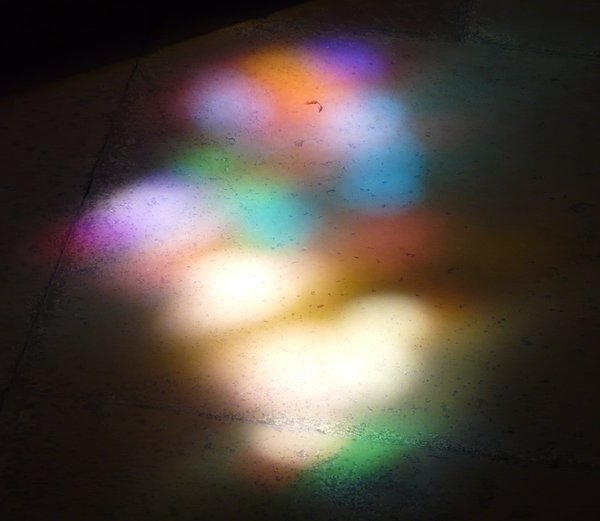
\includegraphics[height=6cm]{lichtspiel.jpg}}
\end{dispListing}
{\tcbset{reset}\tcbusetemp}

\end{docTcbKey}


\begin{docTcbKeys}[
    doc parameter   = {=\marg{code}},
    doc description = {无默认值，初始为空},
    doc new         = 2022-06-21,
  ]
  {
    {
      doc name        = before float,
    },
    {
      doc name        = after float,
    }
  }
  对于浮动对象，\refKey{/tcb/before} 和 \refKey{/tcb/after} 设置被忽略。
  可用 \refKey{/tcb/before float} 在浮动环境开始之后、
  \refKey{/tcb/every float} 之前插入代码；
  用 \refKey{/tcb/after float} 在文本框结束之后、浮动环境结束之前插入代码。
  \begin{marker}
  这些选项与 \refKey{/tcb/breakable} 浮动对象不兼容；
  若文本框设为可断开，则被忽略。
  \end{marker}
\end{docTcbKeys}




\clearpage
\subsection{嵌入上下文}\label{subsec:surroundings}
通常（但不必须），|tcolorbox| 放在独立段落中，前后留有垂直间距。
此行为由键 \refKey{/tcb/before} 和 \refKey{/tcb/after} 控制。

\begin{marker}
4.40 版本之前，\refKey{/tcb/before} 和 \refKey{/tcb/after} 的默认值
由 \refKey{/tcb/autoparskip} 给出。从 4.40 版本起，默认值改由
\refKey{/tcb/before skip balanced} 和 \refKey{/tcb/after skip balanced} 给出。\par
注意：旧文档可能需要调整分页。\par
或者，可在文档导言区使用下面的写法恢复旧默认值：
\begin{dispListing}
\tcbsetforeverylayer{autoparskip}
\end{dispListing}
\end{marker}


\begin{docTcbKey}{before}{=\meta{code}}{无默认值，初始见 \refKey{/tcb/before skip balanced}}
  设置在彩色文本框之前执行的 \meta{代码}。浮动文本框不使用此设置。
  此外，若文本框紧跟在标题之后且 \refKey{/tcb/ignore nobreak} 设为 \docValue{false}，
  也不使用。
\end{docTcbKey}

\begin{docTcbKey}{after}{=\meta{code}}{无默认值，初始见 \refKey{/tcb/after skip balanced}}
  设置在彩色文本框之后执行的 \meta{代码}。浮动文本框不使用此设置。
\end{docTcbKey}


\begin{docTcbKey}{nobeforeafter}{}{样式，无取值}
  清空 |before| 和 |after| 键的缩写。
  彩色文本框不放入段落，前后也不留间距。
\begin{exdispExample}{nobeforeafter}
\tcbset{myone/.style={colback=LightGreen,colframe=DarkGreen,
  equal height group=nobefaf,width=\linewidth/4,nobeforeafter}}
\begin{tcolorbox}[myone,title=Box 1]Box 1\end{tcolorbox}%
\begin{tcolorbox}[myone,title=Box 2]Box 2\end{tcolorbox}%
\begin{tcolorbox}[myone,title=Box 3]Box 3\end{tcolorbox}%
\begin{tcolorbox}[myone,title=Box 4]Box 4\end{tcolorbox}
\end{exdispExample}
\end{docTcbKey}

\begin{docTcbKey}{force nobeforeafter}{}{样式，无取值}
  即使之后 \refKey{/tcb/before} 和 \refKey{/tcb/after} 被设为其他值，
  也强制保持 \refKey{/tcb/nobeforeafter} 的设置。
  除非\emph{确实}清楚自己在做什么，否则不要全局使用此选项。
  注意：嵌套文本框不继承这种强制间距设置。
\end{docTcbKey}


\clearpage

\begin{docTcbKey}[][doc new={2020-09-25}]{before skip balanced}{=\meta{glue}}{无默认值，初始 |0.5\textbackslash baselineskip plus 2pt|}
  在彩色文本框前插入垂直间距。此样式设置 \refKey{/tcb/before}。\par
  若前一个 \TeX\ 盒子的深度在 |0pt| 到 |0.3\baselineskip| 之间，
  则前一个 \TeX\ 盒子的\emph{基线}到 tcolorbox 的距离设为
  \meta{glue}$+$|0.3\baselineskip|。\par
  若深度更大，则前一个 \TeX\ 盒子到 tcolorbox 的距离设为 \meta{glue}。\par
  另见忽略\emph{基线}的 \refKey{/tcb/before skip}。

\begin{exdispExample*}{before_skip_balanced}{sbs,lefthand ratio=0.6}
Some text.
\begin{tcolorbox}[before skip balanced=1cm,
    colframe=red!50!white]
  This is a \textbf{tcolorbox}.
\end{tcolorbox}
\end{exdispExample*}
\end{docTcbKey}

\begin{docTcbKey}[][doc new={2020-09-25}]{after skip balanced}{=\meta{glue}}{无默认值，初始 |0.5\textbackslash baselineskip plus 2pt|}
  在彩色文本框后插入给定 \meta{glue} 的垂直间距。此样式设置 \refKey{/tcb/after}。
  此外，|\prevdepth| 设为 |0.3\baselineskip|。
  后续 \TeX\ 盒子可通过额外弹性间距扩大此距离以调整其\emph{基线}。
  另见忽略\emph{基线}的 \refKey{/tcb/after skip}。

\begin{exdispExample*}{after_skip_balanced}{sbs,lefthand ratio=0.6}
\begin{tcolorbox}[after skip balanced=1cm,
    colframe=red!50!white]
  This is a \textbf{tcolorbox}.
\end{tcolorbox}
Some text.
\end{exdispExample*}
\end{docTcbKey}


\begin{docTcbKey}[][doc new={2020-09-25}]{beforeafter skip balanced}{=\meta{glue}}{无默认值，初始 |0.5\textbackslash baselineskip plus 2pt|}
  在彩色文本框\emph{前后}都插入给定 \meta{glue} 的垂直间距。
  此样式设置 \refKey{/tcb/before skip balanced} 和 \refKey{/tcb/after skip balanced}。
\begin{exdispExample*}{beforeafter_skip_balanced}{sbs,lefthand ratio=0.6}
\newtcolorbox{doubleline}[1][]{
  beforeafter skip balanced=0pt,
  height=1.8\baselineskip,
  enlarge top by=.1\baselineskip,
  enlarge bottom by=.1\baselineskip,
  colframe=blue!20,colback=blue!5,
  size=small,valign upper=center,#1 }

\noindent\begin{tikzpicture}
\path[use as bounding box] (0,0)
  rectangle (0.1,0.1);
\foreach \y in {0,1,...,9}  {
  \draw[very thin,red]
    (-0.2,-\y*\baselineskip) --
    (\linewidth+0.2cm,-\y*\baselineskip); }
\end{tikzpicture}
line 1\par
\begin{doubleline}  Abc  \end{doubleline}
\begin{doubleline}  Def  \end{doubleline}
line 2g\par
\begin{doubleline}  Ghi  \end{doubleline}
line 3\par
line 4 g
\end{exdispExample*}
\end{docTcbKey}


\clearpage

\begin{docTcbKey}[][doc new and updated={2020-09-25}{2015-03-16}]{before skip}{=\meta{glue}}{样式，无默认值}
  在彩色文本框前插入给定 \meta{弹性间距} 的垂直间距。
  此样式设置 \refKey{/tcb/before}。
  与 \refKey{/tcb/before skip balanced} 不同，
  此 \meta{弹性间距} 相对于前一个文本框的下边缘，而非基线。
\begin{exdispExample*}{before_skip}{sbs,lefthand ratio=0.6}
Some text.
\begin{tcolorbox}[before skip=1cm,
    colframe=red!50!white]
  This is a \textbf{tcolorbox}.
\end{tcolorbox}
\end{exdispExample*}
\end{docTcbKey}

\begin{docTcbKey}[][doc new and updated={2020-09-25}{2017-02-01}]{after skip}{=\meta{glue}}{样式，无默认值}
  在彩色文本框后插入给定 \meta{glue} 的垂直间距。此样式设置 \refKey{/tcb/after}。
  与 \refKey{/tcb/after skip balanced} 不同，此 \meta{glue} 相对于后续文本框的上边缘，
  而非基线。
\begin{exdispExample*}{after_skip}{sbs,lefthand ratio=0.6}
\begin{tcolorbox}[after skip=1cm,
    colframe=red!50!white]
  This is a \textbf{tcolorbox}.
\end{tcolorbox}
Some text.
\end{exdispExample*}
\end{docTcbKey}

\begin{docTcbKey}[][doc new=2014-10-10]{beforeafter skip}{=\meta{glue}}{样式，无默认值}
  在彩色文本框\emph{前后}都插入给定 \meta{glue} 的垂直间距。
  此样式设置 \refKey{/tcb/before skip} 和 \refKey{/tcb/after skip}。
\begin{exdispExample*}{beforeafter_skip}{sbs,lefthand ratio=0.6}
\tcbset{beforeafter skip=0pt,
  colframe=red!50!white}

text before
\begin{tcolorbox}
  This is a \textbf{tcolorbox}.
\end{tcolorbox}
\begin{tcolorbox}
  Second box.
\end{tcolorbox}
text after
\end{exdispExample*}
\end{docTcbKey}


\clearpage

\begin{docTcbKey}[][doc new=2014-11-07]{left skip}{=\meta{length}}{样式，无默认值，初始 |0mm|}
  在彩色文本框前插入给定 \meta{长度} 的水平间距。
  此样式将 \refKey{/tcb/grow to left by} 设为取负后的 \meta{长度}，
  即包围盒和文本框宽度都会改变。
\begin{exdispExample*}{left_skip}{sbs,lefthand ratio=0.6}
\noindent\rule{\linewidth}{2pt}

\begin{tcolorbox}[left skip=1cm,
    colframe=red!50!white]
  This is a \textbf{tcolorbox}.
\end{tcolorbox}
\end{exdispExample*}
\end{docTcbKey}

\begin{docTcbKey}[][doc new=2014-11-07]{right skip}{=\meta{length}}{样式，无默认值，初始 |0mm|}
  在彩色文本框后插入给定 \meta{长度} 的水平间距。
  此样式将 \refKey{/tcb/grow to right by} 设为取负后的 \meta{长度}，
  即包围盒和文本框宽度都会改变。
\begin{exdispExample*}{right_skip}{sbs,lefthand ratio=0.6}
\noindent\rule{\linewidth}{2pt}

\begin{tcolorbox}[right skip=1cm,
    colframe=red!50!white]
  This is a \textbf{tcolorbox}.
\end{tcolorbox}
\end{exdispExample*}
\end{docTcbKey}

\begin{docTcbKey}[][doc new=2014-10-10]{leftright skip}{=\meta{length}}{样式，无默认值}
  在彩色文本框\emph{前后}都插入给定 \meta{长度} 的水平间距。
  此样式会改变包围盒和文本框宽度。
\begin{exdispExample*}{leftright_skip}{sbs,lefthand ratio=0.6}
\noindent\rule{\linewidth}{2pt}

\begin{tcolorbox}[leftright skip=1cm,
    colframe=red!50!white]
  This is a \textbf{tcolorbox}.
\end{tcolorbox}
\end{exdispExample*}
\end{docTcbKey}


\clearpage

\begin{docTcbKey}[][doc updated=2017-02-01]{parskip}{}{样式，无取值}
  此选项已被 \refKey{/tcb/before skip balanced} 和 \refKey{/tcb/after skip balanced}
  取代（见第~\pageref{subsec:surroundings}~页的注释）。\par
  当\emph{使用}了 \refPkg{parskip} 宏包且对 |before| 和 |after| 没有更好的设置时，
  将 |before| 和 |after| 键设为推荐值。等价于：
\begin{dispListing}
\tcbset{parskip/.style={before={\par\pagebreak[0]\parindent=0pt},
                        after={\par}}}
\end{dispListing}
\end{docTcbKey}

\begin{docTcbKey}[][doc updated=2017-02-01]{noparskip}{}{样式，无取值}
  此选项已被 \refKey{/tcb/before skip balanced} 和 \refKey{/tcb/after skip balanced}
  取代（见第~\pageref{subsec:surroundings}~页的注释）。\par
  当\emph{未使用} \refPkg{parskip} 宏包且对 |before| 和 |after| 没有更好的设置时，
  将 |before| 和 |after| 键设为推荐值。等价于：
\begin{dispListing}
\tcbset{noparskip/.style={before={\par\pagebreak[0]\smallskip\parindent=0pt},
                          after={\par\smallskip}}}
\end{dispListing}
\end{docTcbKey}

\begin{docTcbKey}{autoparskip}{}{样式，无取值}
  此选项已被 \refKey{/tcb/before skip balanced} 和 \refKey{/tcb/after skip balanced}
  取代（见第~\pageref{subsec:surroundings}~页的注释）。\par
  自动检测是否使用了 \refPkg{parskip} 宏包，并相应设置 |before| 和 |after| 键。
  具体做法如下：
  \begin{itemize}
  \item 若文档开头时 |\parskip| 的长度大于 |0pt|，则执行 \refKey{/tcb/parskip}。
    此处\emph{假定}使用了 \refPkg{parskip} 宏包。
  \item 否则，若文档开头时 |\parskip| 的长度不大于 |0pt|，则执行 \refKey{/tcb/noparskip}。
    此处\emph{假定}未使用 \refPkg{parskip} 宏包。
  \end{itemize}
\end{docTcbKey}


\clearpage

\begin{docTcbKey}{baseline}{=\meta{length}}{无默认值，初始 |0pt|}
  用于设置所得 |tcolorbox| 的 |\pgfsetbaseline| 值。
\begin{exdispExample}{baseline}
\tcbset{colframe=red!50!white,width=4cm,nobeforeafter}
Some text\dotfill
\begin{tcolorbox}[baseline=3mm]
One line.
\end{tcolorbox}
\begin{tcolorbox}[baseline=3mm]
First line.\\Second line.
\end{tcolorbox}
\end{exdispExample}
\end{docTcbKey}


\begin{docTcbKey}[][doc new=2014-10-10]{box align}{=\meta{alignment}}{样式，无默认值，初始 |bottom|}
  用于设置所得 |tcolorbox| 的 \refKey{/tcb/baseline} 值。
  \meta{alignment} 的可用取值为：
  \begin{itemize}
  \item\docValue{bottom}：与文本框底部对齐，
  \item\docValue{top}：与文本框顶部对齐，
  \item\docValue{center}：与文本框中心对齐，
  \item\docValue{base}：与文本框内容基线对齐。此选项不适用于 \refEnv{tcolorbox}，
    仅适用于 \refCom{tcbox}。它是 \refKey{/tcb/tcbox raise base} 的别名。
  \end{itemize}

\begin{exdispExample}{box_align_1}
\tcbset{colframe=red!50!white,width=4cm,nobeforeafter}
Some text\dotfill
\begin{tcolorbox}[box align=bottom]
One line.
\end{tcolorbox}
\begin{tcolorbox}[box align=bottom]
First line.\\Second line.
\end{tcolorbox}
\end{exdispExample}

\begin{exdispExample}{box_align_2}
\tcbset{colframe=red!50!white,width=4cm,nobeforeafter}
Some text\dotfill
\begin{tcolorbox}[box align=top]
One line.
\end{tcolorbox}
\begin{tcolorbox}[box align=top]
First line.\\Second line.
\end{tcolorbox}
\end{exdispExample}

\begin{exdispExample}{box_align_3}
\tcbset{colframe=red!50!white,width=4cm,nobeforeafter}
Some text\dotfill
\begin{tcolorbox}[box align=center]
One line.
\end{tcolorbox}
\begin{tcolorbox}[box align=center]
First line.\\Second line.
\end{tcolorbox}
\end{exdispExample}

\begin{exdispExample}{box_align_4}
\tcbset{colframe=red!50!white,nobeforeafter}
Some text\dotfill
\tcbox[nobeforeafter,box align=base]{One line}
\tcbox[nobeforeafter,box align=base,size=fbox]{Another line}
\end{exdispExample}
\end{docTcbKey}




\begin{docTcbKey}[][doc new=2014-12-11]{ignore nobreak}{\colOpt{=true\textbar false}}{默认 |true|，初始 |false|}
标题之后，\LaTeX\ 会设置 |nobreak| 布尔值以避免断行。
从 |3.33| 版本起，若 \refKey{/tcb/ignore nobreak} 设为 \docValue{false}，
则标题之后不使用 \refKey{/tcb/before} 或 \refKey{/tcb/before skip} 设置。
对于不可断开的文本框，改用 \refKey{/tcb/before nobreak}。
此外，\refKey{/tcb/breakable} 文本框也会尽量避免
在标题与紧随其后的断开序列第一部分之间断页。

若要像 |3.33| 版本之前那样忽略 |nobreak|，
可将 \refKey{/tcb/ignore nobreak} 设为 \docValue{true}。
此设置也可在局部使用，以强制应用 \refKey{/tcb/before} 设置。
\end{docTcbKey}

\begin{docTcbKey}[][doc new=2014-12-16]{before nobreak}{=\meta{code}}{无默认值，初始 \cs{noindent}}
  当彩色文本框不可断开、未设置 \refKey{/tcb/ignore nobreak}
  且文本框紧跟在标题之后时，设置在其之前执行的 \meta{代码}。
\end{docTcbKey}


\begin{docTcbKey}[][doc new=2017-02-23]{parfillskip restore}{\colOpt{=true\textbar false}}{默认 |true|，初始 |true|}
  若此选项设为 |true|，则在特定位置检查 |\parfillskip| 的最小值是否大于 |0pt|。
  若是，则将 |\parfillskip| 恢复为 |\@flushglue|（恰好是默认值）。
  这些检查会在 \refKey{/tcb/parskip}、\refKey{/tcb/noparskip}、
  \refKey{/tcb/after skip}、\refKey{/tcb/breakable} 和 \refEnv{tcbraster} 处执行。
  此选项用于在使用会改变 |\parfillskip| 的宏包时，
  自动避免 overfull box 警告。
\end{docTcbKey}



\clearpage
\subsection{包围盒}
通常，每个 |tcolorbox| 的包围盒恰好与外边框尺寸一致。
因此 \LaTeX\ 只会为文本框预留所需空间。
可以通过扩大（或缩小）包围盒来改变此行为。
扩大包围盒时，|tcolorbox| 周围会多出间距。
缩小包围盒（即用负值扩大）时，|tcolorbox| 会与页面其他部分重叠，
例如可延伸到页边距中。

\begin{marker}
下面的示例使用 \refKey{/tcb/show bounding box} 显示实际包围盒。
为此需加载 \mylib{skins} 程序库并设置 \refKey{/tcb/enhanced}。
\end{marker}

\subsubsection{移动包围盒边界}

\begin{docTcbKey}{enlarge top initially by}{=\meta{length}}{无默认值，初始 |0mm|}
  将包围盒到文本框顶部的距离扩大 \meta{长度}。
  若文本框\emph{可断开}，则仅断开序列的第一个文本框被扩大。
  \refKey{/tcb/enlarge top by} 会覆盖此键。
\begin{exdispExample}{enlarge_top_initially_by}
\tcbset{colframe=blue!75!black,colback=white}

\begin{tcolorbox}[enlarge top initially by=-5mm]
This is a \textbf{tcolorbox}.
\end{tcolorbox}
\begin{tcolorbox}[enlarge top initially by=5mm,enhanced,show bounding box]
This is a \textbf{tcolorbox}.
\end{tcolorbox}
\end{exdispExample}
\end{docTcbKey}



\begin{docTcbKey}{enlarge bottom finally by}{=\meta{length}}{无默认值，初始 |0mm|}
  将包围盒到文本框底部的距离扩大 \meta{长度}。
  若文本框\emph{可断开}，则仅断开序列的最后一个文本框被扩大。
  \refKey{/tcb/enlarge bottom by} 会覆盖此键。
\begin{exdispExample}{enlarge_bottom_finally_by}
\tcbset{colframe=blue!75!black,colback=white}

\begin{tcolorbox}[enlarge bottom finally by=5mm]
This is a \textbf{tcolorbox}.
\end{tcolorbox}
\begin{tcolorbox}[enlarge bottom finally by=-5mm,enhanced,show bounding box]
This is a \textbf{tcolorbox}.
\end{tcolorbox}
\end{exdispExample}
\end{docTcbKey}

\clearpage


\begin{docTcbKey}{enlarge top at break by}{=\meta{length}}{无默认值，初始 \texttt{0mm}}
  若文本框为 \refKey{/tcb/breakable}，
  则将包围盒到文本框顶部的距离扩大 \meta{长度}。
  此时作用于断开序列的\emph{中间}和\emph{最后}部分。
  \refKey{/tcb/enlarge top by} 会覆盖此键。
\end{docTcbKey}


\begin{docTcbKey}{enlarge bottom at break by}{=\meta{length}}{无默认值，初始 \texttt{0mm}}
  若文本框为 \refKey{/tcb/breakable}，
  则将包围盒到文本框底部的距离扩大 \meta{长度}。
  此时作用于断开序列的\emph{第一}和\emph{中间}部分。
  \refKey{/tcb/enlarge bottom by} 会覆盖此键。
\end{docTcbKey}


\begin{docTcbKey}{enlarge top by}{=\meta{length}}{无默认值，初始 |0mm|}
  将包围盒到文本框顶部的距离扩大 \meta{长度}。
  同时将 \refKey{/tcb/enlarge top initially by} 和 \refKey{/tcb/enlarge top at break by}
  设为 \meta{长度}。
\end{docTcbKey}


\begin{docTcbKey}{enlarge bottom by}{=\meta{length}}{无默认值，初始 |0mm|}
  将包围盒到文本框底部的距离扩大 \meta{长度}。
  同时将 \refKey{/tcb/enlarge bottom finally by} 和 \refKey{/tcb/enlarge bottom at break by}
  设为 \meta{长度}。
\end{docTcbKey}


\begin{docTcbKey}{enlarge left by}{=\meta{length}}{无默认值，初始 |0mm|}
  将包围盒到文本框左侧的距离扩大 \meta{长度}。
\begin{exdispExample}[safety=2cm]{enlarge_left_by}
\tcbset{colframe=blue!75!black,colback=white}

\begin{tcolorbox}[enlarge left by=2cm,width=5cm,enhanced,show bounding box]
This is a \textbf{tcolorbox}.
\end{tcolorbox}
\begin{tcolorbox}[enlarge left by=-2cm,width=\linewidth+2cm]
This is a \textbf{tcolorbox}.
\end{tcolorbox}
\end{exdispExample}
\end{docTcbKey}

\begin{docTcbKey}{enlarge right by}{=\meta{length}}{无默认值，初始 |0mm|}
  将包围盒到文本框右侧的距离扩大 \meta{长度}。
\begin{exdispExample}[safety=2cm]{enlarge_right_by}
\tcbset{colframe=blue!75!black,colback=white}

\begin{tcolorbox}[enlarge right by=-2cm,width=\linewidth+2cm,
  enhanced,show bounding box]
This is a \textbf{tcolorbox}.
\end{tcolorbox}
\begin{tcolorbox}[enlarge right by=2cm,width=\linewidth-2cm]
This is a \textbf{tcolorbox}.
\end{tcolorbox}
\end{exdispExample}
\end{docTcbKey}

\clearpage
\begin{docTcbKey}{enlarge by}{=\meta{length}}{无默认值，初始 |0mm|}
  将包围盒到文本框各边的距离都扩大 \meta{长度}。
\begin{exdispExample}{enlarge_by}
\tcbset{colframe=blue!75!black,colback=white,width=5cm,nobeforeafter}

\begin{tcolorbox}
This is a \textbf{tcolorbox}.
\end{tcolorbox}
\begin{tcolorbox}[enlarge by=5mm,enhanced,show bounding box]
This is a \textbf{tcolorbox}.
\end{tcolorbox}
\end{exdispExample}
\end{docTcbKey}



\begin{docTcbKey}{grow to left by}{=\meta{length}}{无默认值，初始 |0mm|}
  将当前文本框宽度扩大 \meta{长度}，
  并将包围盒到文本框左侧的距离扩大 $-$\meta{长度}（即缩小）。
  另见 \refKey{/tcb/left skip}。
\begin{exdispExample}[safety=2cm]{grow_to_left_by}
\tcbset{colframe=blue!75!black,colback=white}

\begin{tcolorbox}[width=5cm,grow to left by=2cm,enhanced,show bounding box]
This is a \textbf{tcolorbox} with a width of 7cm.
\end{tcolorbox}
\end{exdispExample}
\end{docTcbKey}

\begin{docTcbKey}{grow to right by}{=\meta{length}}{无默认值，初始 |0mm|}
  将当前文本框宽度扩大 \meta{长度}，
  并将包围盒到文本框右侧的距离扩大 $-$\meta{长度}（即缩小）。
  另见 \refKey{/tcb/right skip}。
\begin{exdispExample}[safety=2cm]{grow_to_right_by}
\tcbset{colframe=blue!75!black,colback=white}

\begin{tcolorbox}[grow to right by=2cm,enhanced,show bounding box]
This is a \textbf{tcolorbox}.
\end{tcolorbox}

\bigskip

\begin{tcolorbox}[grow to right by=2cm,grow to left by=1cm,
  enhanced,show bounding box]
This is a \textbf{tcolorbox}.
\end{tcolorbox}
\end{exdispExample}
\end{docTcbKey}

\clearpage

\begin{docTcbKey}[][doc new=2018-03-22]{grow sidewards by}{=\meta{length}}{无默认值，初始 |0mm|}
  将 \refKey{/tcb/grow to left by} 和 \refKey{/tcb/grow to right by}
  都设为 \meta{长度} 的快捷方式。
  另见 \refKey{/tcb/oversize} 和 \refKey{/tcb/spread sidewards}。
\begin{exdispExample}[safety=2cm]{grow_sidewards_by}
\tcbset{colframe=blue!75!black,colback=white}

\begin{tcolorbox}[grow sidewards by=2cm,enhanced,show bounding box]
This is a \textbf{tcolorbox}.
\end{tcolorbox}
\end{exdispExample}
\end{docTcbKey}


\subsubsection{文本框对齐}

\begin{docTcbKey}[][doc new=2015-11-20]{flush left}{}{样式，无取值}
  将包围盒向右侧扩大，直到占满整行。
\begin{exdispExample}{flush_left}
\tcbset{colframe=blue!75!black,colback=white}

\begin{tcolorbox}[flush left,width=5cm,enhanced,show bounding box]
This is a \textbf{tcolorbox}.
\end{tcolorbox}
\end{exdispExample}
\end{docTcbKey}


\begin{docTcbKey}[][doc new=2015-11-20]{flush right}{}{样式，无取值}
  将包围盒向左侧扩大，直到占满整行。
\begin{exdispExample}{flush_right}
\tcbset{colframe=blue!75!black,colback=white}

\begin{tcolorbox}[flush right,width=5cm,enhanced,show bounding box]
This is a \textbf{tcolorbox}.
\end{tcolorbox}
\end{exdispExample}
\end{docTcbKey}


\begin{docTcbKey}[][doc new=2015-11-20]{center}{}{样式，无取值}
  将包围盒向两侧等量扩大，直到占满整行。
\begin{exdispExample}{center}
\tcbset{colframe=blue!75!black,colback=white}

\begin{tcolorbox}[center,width=5cm,enhanced,show bounding box]
This is a \textbf{tcolorbox}.
\end{tcolorbox}
\end{exdispExample}
\end{docTcbKey}


\clearpage
\subsubsection{切换扩缩}

\begin{docTcbKey}[][doc updated=2015-11-13]{toggle enlargement}{=\meta{toggle preset}}{默认 |evenpage|，初始 |none|}
  根据 \meta{切换预设}，决定是否切换包围盒的左右扩缩。可用取值为：
  \begin{itemize}
  \item\docValue{none}：不切换。
  \item\docValue{forced}：切换左右扩缩的取值。
  \item\docValue{evenpage}：若当前页为偶数页，则切换左右扩缩的取值。
    此取值同时将 \refKey{/tcb/check odd page} 设为 |true|。
  \end{itemize}
\begin{marker}
切换几何设置见 \refKey{/tcb/toggle left and right}。
\end{marker}

\begin{dispExample}
\tcbset{colframe=blue!75!black,colback=white,
  grow to left by=20mm,grow to right by=-5mm}

\begin{tcolorbox}[toggle enlargement=none,enhanced,show bounding box]
This is a \textbf{tcolorbox}.
\end{tcolorbox}
\begin{tcolorbox}[toggle enlargement=forced]
This is a \textbf{tcolorbox}.
\end{tcolorbox}
\begin{tcolorbox}[toggle enlargement=evenpage]
  This page is an \tcbifoddpage{odd}{even} page.
  Therefore, the left and right enlargements
  \tcbifoddpage{are not}{are} toggled.
\end{tcolorbox}
\end{dispExample}

\begin{dispListing}
\begin{tcolorbox}[colframe=red!60!black,colback=red!15!white,
  fonttitle=\bfseries,title=Floating box from \texttt{toggle enlargement},
  width=\textwidth,grow to right by=2cm,toggle enlargement,float=t]
  This page is an \tcbifoddpage{odd}{even} page.
  Therefore, the left and right enlargements \tcbifoddpage{are not}{are} toggled.
  This box stretches to the right margin on odd pages and to the left
  margin on even pages. The current document is one-sided -- this feature makes
  sense for two-sided documents only.
\end{tcolorbox}
\end{dispListing}
\tcbusetemp
\end{docTcbKey}



\clearpage
\subsubsection{文本框延伸到页边}

\begin{marker}
下面的页边选项\emph{不}适用于嵌套文本框、表格内文本框等。
列表内文本框\emph{可能}有效，但不保证。
此外，文本框应以 |\noindent| 和全宽设置。
\end{marker}

\begin{docTcbKey}[][doc new=2017-02-13]{spread inwards}{\colOpt{=\meta{length}}}{默认 |0pt|，初始未设置}
将当前文本框宽度扩大到内侧页边距（单栏文档为左侧）。
若可选 \meta{长度} 大于 |0pt|，文本框越过页边；
若 \meta{长度} 小于 |0pt|，文本框与页边之间留间距。
双面文档会自动设置 \refKey{/tcb/toggle enlargement}。
\begin{dispListing}
\begin{tcolorbox}[enhanced,spread inwards,
  colframe=blue!75!black,colback=white,show bounding box]
This is a \textbf{tcolorbox}.
\end{tcolorbox}
\end{dispListing}
{\tcbusetemp}
\end{docTcbKey}

\begin{docTcbKey}[][doc new=2017-02-13]{spread outwards}{\colOpt{=\meta{length}}}{默认 |0pt|，初始未设置}
将当前文本框宽度扩大到外侧页边距（单栏文档为右侧）。
若可选 \meta{长度} 大于 |0pt|，文本框越过页边；
若 \meta{长度} 小于 |0pt|，文本框与页边之间留间距。
双面文档会自动设置 \refKey{/tcb/toggle enlargement}。
\begin{dispListing}
\begin{tcolorbox}[enhanced,spread outwards,
  colframe=blue!75!black,colback=white,show bounding box]
This is a \textbf{tcolorbox}.
\end{tcolorbox}
\end{dispListing}
{\tcbusetemp}
\end{docTcbKey}

\begin{marker}
下面所有垂直延伸选项不适用于可断开文本框！
\end{marker}

\begin{docTcbKey}[][doc new=2017-02-13]{move upwards}{\colOpt{=\meta{length}}}{默认 |0pt|，初始未设置}
  另起一页，将文本框放在页面最顶部的页边。
  若可选 \meta{长度} 大于 |0pt|，文本框越过页边；
  若 \meta{长度} 小于 |0pt|，文本框与页边之间留间距。
\end{docTcbKey}


\begin{docTcbKey}[][doc new=2017-02-13]{move upwards*}{\colOpt{=\meta{length}}}{默认 |0pt|，初始未设置}
  与 \refKey{/tcb/move upwards} 相同，但不另起一页。
\end{docTcbKey}


\begin{docTcbKey}[][doc new=2017-02-13]{fill downwards}{\colOpt{=\meta{length}}}{默认 |0pt|，初始未设置}
  将文本框高度扩大到页面最底部的页边。
  需加载 \mylib{breakable} 程序库，并自动设置 \refKey{/tcb/height fill}。
  若可选 \meta{长度} 大于 |0pt|，文本框越过页边；
  若 \meta{长度} 小于 |0pt|，文本框与页边之间留间距。
\begin{dispListing}
\begin{tcolorbox}[enhanced,fill downwards,
  colframe=blue!75!black,colback=white,show bounding box]
This is a \textbf{tcolorbox}.
\end{tcolorbox}
\end{dispListing}
{\tcbusetemp}
\end{docTcbKey}


\begin{tcolorbox}[enhanced,spread upwards,sharp corners=north,height=3cm,
  colframe=blue!75!black,interior style={top color=blue!50,bottom color=white}]
This is an example for \enquote{spread upwards}.
\end{tcolorbox}
\begin{docTcbKey}[][doc new=2017-02-13]{spread upwards}{\colOpt{=\meta{length}}}{默认 |0pt|，初始未设置}
  \refKey{/tcb/move upwards}、\refKey{/tcb/spread inwards} 和 \refKey{/tcb/spread outwards}
  的组合。可选 \meta{长度} 用于所有这些键。
\begin{dispListing}
\begin{tcolorbox}[enhanced,spread upwards,sharp corners=north,height=3cm,
  colframe=blue!75!black,interior style={top color=blue!50,bottom color=white}]
This is an example for \enquote{spread upwards}.
\end{tcolorbox}
\end{dispListing}
\end{docTcbKey}


\begin{docTcbKey}[][doc new=2017-02-13]{spread upwards*}{\colOpt{=\meta{length}}}{默认 |0pt|，初始未设置}
  与 \refKey{/tcb/move upwards} 相同，但不另起一页。
\end{docTcbKey}


\begin{docTcbKey}[][doc new=2017-02-13]{spread sidewards}{\colOpt{=\meta{length}}}{默认 |0pt|，初始未设置}
  \refKey{/tcb/spread inwards} 和 \refKey{/tcb/spread outwards} 的组合。
  可选 \meta{长度} 用于所有这些键。
  另见 \refKey{/tcb/oversize} 和 \refKey{/tcb/grow sidewards by}。
\begin{dispListing}
\begin{tcolorbox}[enhanced,spread sidewards,
  colframe=blue!75!black,colback=white,show bounding box]
This is a \textbf{tcolorbox}.
\end{tcolorbox}
\end{dispListing}
{\tcbusetemp}
\end{docTcbKey}


\begin{docTcbKey}[][doc new=2017-02-13]{spread}{\colOpt{=\meta{length}}}{默认 |0pt|，初始未设置}
  \refKey{/tcb/move upwards}、\refKey{/tcb/fill downwards}、
  \refKey{/tcb/spread inwards} 和 \refKey{/tcb/spread outwards} 的组合。
  这样文本框会占满整页。可选 \meta{长度} 用于所有这些键。
\end{docTcbKey}


\begin{docTcbKey}[][doc new=2017-02-13]{spread downwards}{\colOpt{=\meta{length}}}{默认 |0pt|，初始未设置}
  \refKey{/tcb/fill downwards}、\refKey{/tcb/spread inwards} 和
  \refKey{/tcb/spread outwards} 的组合。可选 \meta{长度} 用于所有这些键。
\begin{dispListing}
\begin{tcolorbox}[enhanced,spread downwards,sharp corners=south,
  colframe=red!75!black,interior style={top color=white,bottom color=red!50}]
This is an example for \enquote{spread downwards}.
\end{tcolorbox}
\end{dispListing}
\end{docTcbKey}
\begin{tcolorbox}[enhanced,spread downwards,sharp corners=south,
  colframe=red!75!black,interior style={top color=white,bottom color=red!50}]
This is an example for \enquote{spread downwards}.
\end{tcolorbox}




\clearpage
\subsubsection{文本框挤出}

\begin{marker}
下面的键不应与可断开文本框配合使用。
\end{marker}

\begin{docTcbKey}{shrink tight}{}{样式，无取值，初始未设置}
  将整个彩色文本框收缩到上部的尺寸。此时不应有下部和标题。
  此样式将 \refKey{/tcb/boxsep} 设为 |0pt|，
  并将其他几何键设为合适值。
  此选项通常与下面的挤出键配合使用。
\begin{exdispExample}{shrink_tight}
\tcbset{colframe=blue!75!black,colback=white,arc=0mm,boxrule=0.4pt,
        nobeforeafter,tcbox raise base,shrink tight}

\begin{tcolorbox}
This is a \textbf{tcolorbox}.
\end{tcolorbox}

Lorem \tcbox{ipsum} dolor sit amet, consectetuer adipiscing elit.
\end{exdispExample}
\end{docTcbKey}

\begin{docTcbKey}[][doc updated=2014-09-19]{extrude left by}{=\meta{length}}{样式，无默认值，初始未设置}
  将彩色文本框向左侧挤出给定 \meta{长度}。
  内宽和包围盒保持不变，且操作是累加的！
\begin{exdispExample}{extrude_left_by}
\tcbset{enhanced,colframe=red,colback=yellow!25!white,
  frame style={opacity=0.25},interior style={opacity=0.5},
  nobeforeafter,tcbox raise base,shrink tight,extrude by=2mm}

Lorem ipsum dolor sit amet, consectetuer adipiscing elit. Ut purus elit,
vestibulum ut, placerat ac, adipiscing vitae, felis.
\tcbox[extrude left by=1cm]{Curabitur} dictum gravida mauris.
Nam arcu libero, nonummy eget, consectetuer id, vulputate a, magna.
\end{exdispExample}
\end{docTcbKey}

\begin{docTcbKey}[][doc updated=2014-09-19]{extrude right by}{=\meta{length}}{样式，无默认值，初始未设置}
  将彩色文本框向右侧挤出给定 \meta{长度}。
  内宽和包围盒保持不变，且操作是累加的！
\begin{exdispExample}{extrude_right_by}
\tcbset{enhanced,colframe=red,colback=yellow!25!white,
  frame style={opacity=0.25},interior style={opacity=0.5},
  nobeforeafter,tcbox raise base,shrink tight,extrude by=2mm}

Lorem ipsum dolor sit amet, consectetuer adipiscing elit. Ut purus elit,
vestibulum ut, placerat ac, adipiscing vitae, felis.
\tcbox[extrude right by=1cm]{Curabitur} dictum gravida mauris.
Nam arcu libero, nonummy eget, consectetuer id, vulputate a, magna.
\end{exdispExample}
\end{docTcbKey}

\clearpage
\begin{docTcbKey}{extrude top by}{=\meta{length}}{样式，无默认值，初始未设置}
  将彩色文本框向顶部挤出给定 \meta{长度}。
  内宽和包围盒保持不变，且操作是累加的！
\begin{exdispExample}{extrude_top_by}
\tcbset{enhanced,colframe=red,colback=yellow!25!white,
  frame style={opacity=0.25},interior style={opacity=0.5},
  nobeforeafter,tcbox raise base,shrink tight,extrude by=2mm}

Lorem ipsum dolor sit amet, consectetuer adipiscing elit. Ut purus elit,
vestibulum ut, placerat ac, adipiscing vitae, felis.
\tcbox[extrude top by=1cm]{Curabitur} dictum gravida mauris.
Nam arcu libero, nonummy eget, consectetuer id, vulputate a, magna.
\end{exdispExample}
\end{docTcbKey}

\begin{docTcbKey}{extrude bottom by}{=\meta{length}}{样式，无默认值，初始未设置}
  将彩色文本框向底部挤出给定 \meta{长度}。
  内宽和包围盒保持不变，且操作是累加的！
\begin{exdispExample}[safety=1cm]{extrude_bottom_by}
\tcbset{enhanced,colframe=red,colback=yellow!25!white,
  frame style={opacity=0.25},interior style={opacity=0.5},
  nobeforeafter,tcbox raise base,shrink tight,extrude by=2mm}

Lorem ipsum dolor sit amet, consectetuer adipiscing elit. Ut purus elit,
vestibulum ut, placerat ac, adipiscing vitae, felis.
\tcbox[extrude bottom by=1cm]{Curabitur} dictum gravida mauris.
Nam arcu libero, nonummy eget, consectetuer id, vulputate a, magna.
\end{exdispExample}
\end{docTcbKey}

\begin{docTcbKey}{extrude by}{=\meta{length}}{样式，无默认值，初始未设置}
  将彩色文本框向各边挤出给定 \meta{长度}。
  内宽和包围盒保持不变，且操作是累加的！
\begin{exdispExample}{extrude_by}
\tcbset{enhanced,colframe=red,colback=yellow!25!white,
  frame style={opacity=0.25},interior style={opacity=0.5},
  nobeforeafter,tcbox raise base,shrink tight,extrude by=2mm}

Lorem ipsum dolor sit amet, consectetuer adipiscing elit. Ut purus elit,
vestibulum ut, placerat ac, adipiscing vitae, felis. \tcbox{Curabitur} dictum
gravida mauris. \tcbox[colframe=Green,interior style={opacity=0.0}]{Nam}
arcu libero, nonummy eget, consectetuer id, \tcbox{vulputate} a, magna. Donec
vehicula augue eu neque. Pellentesque habitant morbi tristique senectus et netus
et malesuada fames ac turpis egestas. \tcbox{Mauris ut leo.}
\end{exdispExample}
\end{docTcbKey}

\clearpage
\subsection{分层文本框与全局设置}\label{subsec:everybox}
一个 |tcolorbox| 可以包含另一个 |tcolorbox|，依此类推。
宏包用计数器 \docCounter{tcblayer} 跟踪嵌套层级。
计数器值可用于做一些花哨的事情，但切勿自行修改计数器值。

宏包对前四层（即嵌套层级）做了特殊处理，称为托管层。
在托管层中，脚注文字会被管理到正确位置；
还可通过修改 \refKey{/tcb/every box on layer n} 设置随层变化的选项。
如有需要，可将 \refCom{tcbsetmanagedlayers} 设为大于 4 的值
以增加托管层数。

下面这些样式对分层文本框的处理方式有重大影响。
特别注意：嵌套文本框默认会执行 \refKey{/tcb/reset}。
你可以更改这一点，但需自行承担可能出现的意外。

若\emph{未更改}默认值，|tcolorbox| 按以下顺序获得选项。
后给出的选项覆盖先给出的选项。
\begin{enumerate}
\item 宏包加载时，所有选项设为默认值。
\item 每条 \refCom{tcbset} 命令在当前 \TeX\ 组内为后续文本框添加或更改选项。
\item 进入 |tcolorbox| 时，应用 \refKey{/tcb/every box on layer n} 或
  \refKey{/tcb/every box on higher layers} 选项列表。默认设置下：
  \begin{itemize}
  \item 第 1 层（最内层）应用 \refKey{/tcb/every box} 选项列表。
    此前 \refCom{tcbset} 给出的、未被覆盖的选项保留。
  \item 第 2 层及以上（嵌套文本框）先执行 \refKey{/tcb/reset}，
    再应用 \refKey{/tcb/every box} 选项列表。
    此前 \refCom{tcbset} 及外层文本框给出的所有可重置选项都被重置。
  \end{itemize}
\item 应用传给 |tcolorbox| 的 \meta{选项}。
  若文本框由 \refCom{newtcolorbox} 等命令生成，则应用那些命令给出的 \meta{选项}。
\item 若文本框由 \refCom{newtcolorbox} 等命令生成，还会应用一些自动选项。
\end{enumerate}


\begin{docTcbKey}{every box}{}{样式}
默认情况下，此样式为空。
\begin{dispListing}
% 默认设置：
\tcbset{every box/.style={}}
\end{dispListing}
可通过重新定义此样式来更改。
\begin{dispListing}
% 将所有文本框设为 enhanced：
\tcbset{every box/.style={enhanced}}
\end{dispListing}

\medskip
\begin{marker}
为每个（每层）文本框统一设置选项的另一种方式是使用
\refCom{tcbsetforeverylayer}：
\begin{dispListing}
% 将所有文本框设为 enhanced：
\tcbsetforeverylayer{enhanced}
\end{dispListing}
\end{marker}
\end{docTcbKey}

\clearpage
\begin{docTcbKey}{every box on layer n}{}{样式}
其中，|n| 需替换为 1 到最高托管层号之间的数字（默认为 4）。
\begin{dispListing}
% default settings:
\tcbset{
  every box on layer 1/.style={every box},
  every box on layer 2/.style={reset,every box},
  every box on layer 3/.style={reset,every box},
  every box on layer 4/.style={reset,every box},
  }
\end{dispListing}
\end{docTcbKey}


\begin{docTcbKey}{every box on higher layers}{}{样式}
高层指高于最高托管层号的层级（默认为 4）。
\begin{dispListing}
% default setting:
\tcbset{every box on higher layers/.style={reset,every box}}
\end{dispListing}
\end{docTcbKey}


\begin{docCommand}{tcbsetmanagedlayers}{\marg{number}}
  将最高托管层号改为 \meta{number}，默认为 4。
  此宏只能在导言区使用。取小于 4 的 \meta{number} 通常没有意义，但不禁止。
\end{docCommand}

\begin{tcboutputlisting}
% \usepackage{lipsum}   \tcbuselibrary{skins,breakable}
\tcbset{colframe=red!75!black,fonttitle=\bfseries,
  colback=red!5!white,
  every box/.style={enhanced,watermark text=\thetcblayer,
    before=\par\smallskip,after=\par\smallskip},
  every box on layer 2/.append style={colback=yellow!10!white,drop fuzzy shadow}}
\begin{tcolorbox}[enhanced jigsaw,breakable,title=Layer 1 Box]
Here comes a footnote\footnote{Footnote from layer 1 box}.
\lipsum[2]
  \begin{tcolorbox}[title=Layer 2 Box]
  abc\footnote{The footnote of abc}
  \end{tcolorbox}
  \begin{tcolorbox}[title=Another Box,ams equation]
    \tcbhighmath{\sum\limits_{n=1}^{\infty} \frac{1}{n}} = \infty.
  \end{tcolorbox}
Some text\footnote{Footnote from some text}.
  \begin{tcolorbox}[title=Yet Another Box]
    \tcboxfit[height=2cm]{\lipsum[1]}
    My text.
    \begin{tcolorbox}
      Another lipsum text\footnote{A lipsum text}. \lipsum[3]
      \begin{tcolorbox}[title=Layer 4,colframe=blue,colback=white]
        Layer 4\footnote{Layer 4 footnote}
      \end{tcolorbox}
      The End\footnote{Last footnote}.
    \end{tcolorbox}
  \end{tcolorbox}
\end{tcolorbox}
\end{tcboutputlisting}

\tcbinputlisting{base example,listing only,listing style=mydocumentation}

{\tcbuselistingtext}


\clearpage
\subsection{捕获模式}\label{subsec:capture}

\begin{docTcbKey}{capture}{=\meta{mode}}{无默认值，初始 |minipage|}
  捕获 \meta{模式} 定义文本框内容的处理方式。

\meta{模式} 的可用取值为：
\begin{itemize}
\item\docValue{minipage}：\\
  \refEnv{tcolorbox} 的默认 \meta{模式}。
  内容可分为上部和下部，文本框可选地为 \refKey{/tcb/breakable}。
  文本框内容放入 minipage 或类似 minipage 的环境。
\item\docValue{hbox}：\\
  \refCom{tcbox} 的默认 \meta{模式}。内容不能有下部，也不能断开。
  彩色文本框按内容尺寸确定大小。
  设置此模式的快捷方式是 \refKey{/tcb/hbox}。
\item\docValue{fitbox}：（需 \mylib{fitting} 程序库）\\
  \refCom{tcboxfit} 的默认 \meta{模式}。内容不能有下部，也不能断开。
  内容按彩色文本框尺寸缩放。
  设置此模式的快捷方式是 \refKey{/tcb/fit}。
\end{itemize}

\begin{exdispExample}{capture}
\tcbset{colframe=blue!75!black,colback=white}

\begin{tcolorbox}[capture=minipage]
This is a tcolorbox.
\end{tcolorbox}

\begin{tcolorbox}[capture=hbox]
This is a tcolorbox.
\end{tcolorbox}

\begin{tcolorbox}[capture=fitbox,height=9mm]% needs the `fitting' library
This is a tcolorbox.
\end{tcolorbox}
\end{exdispExample}
\end{docTcbKey}



\begin{docTcbKey}{hbox}{}{样式，无默认值}
  |capture=hbox| 的快捷方式。
\begin{exdispExample}{hbox}
\tcbset{colframe=blue!75!black,colback=white}

\begin{tcolorbox}[hbox]
This is a tcolorbox.
\end{tcolorbox}
\end{exdispExample}
\end{docTcbKey}


\begin{docTcbKey}{minipage}{}{样式，无默认值}
  |capture=minipage| 的快捷方式。
\end{docTcbKey}


\clearpage
\subsection{文字特性}
\begin{docTcbKey}[][doc updated=2024-01-10]{parbox}{\colOpt{=true\textbar false}}{默认 |true|，初始 |true|}
  不可断开的 |tcolorbox| 内文字用 \LaTeX\ |minipage| 排版。
  若可断开，则模拟 |minipage| 行为。
  在 |minipage| 或 |parbox| 中，段落排版与正文略有不同。
  若将此键设为 |false|，则恢复正文的正常行为。
  某些情况下这会产生不期望的副作用。
  建议仅在确实需要此特性时才使用这个\textbf{实验性设置}。
\end{docTcbKey}

\begin{dispListing}
% \usepackage{lipsum}  % preamble
\tcbset{width=(\linewidth-2mm)/2,nobeforeafter,arc=1mm,
  colframe=blue!75!black,colback=white,fonttitle=\bfseries,fontupper=\small,
  left=2mm,right=2mm,top=1mm,bottom=1mm,equal height group=parbox}

\begin{tcolorbox}[parbox,adjusted title={parbox=true (normal)}]
  \lipsum[1-2]
\end{tcolorbox}\hfill%
\begin{tcolorbox}[parbox=false,adjusted title={parbox=false}]
  \lipsum[1-2]
\end{tcolorbox}%
\end{dispListing}
{\tcbusetemp}


\clearpage
\begin{docTcbKey}{hyphenationfix}{\colOpt{=true\textbar false}}{默认 |true|，初始 |false|}
  使用 |pdflatex| 时，极窄文本框中段落开头的长单词不会被断字。
  应用 |hyphenationfix| 选项可绕开此问题。

\begin{exdispExample*}{hyphenationfix}{sbs,lefthand ratio=0.6}
\tcbset{colframe=blue!75!black,
  fontupper=\normalsize,
  colback=blue!5!white,width=4cm}

\begin{tcolorbox}
Rechnungsadjunktentochter.\par
Statthaltereikonzipist.
\end{tcolorbox}

\begin{tcolorbox}[hyphenationfix]
Rechnungsadjunktentochter.\par
Statthaltereikonzipist.
\end{tcolorbox}
\end{exdispExample*}

\smallskip
\begin{marker}
|parbox=false| 与 |hyphenationfix| 不应同时使用。
它们针对不同类型的文本框，配合效果不佳。
\end{marker}
\end{docTcbKey}


\subsection{文件}
\begin{docTcbKey}{tempfile}{=\meta{file name}}{无默认值，初始 \cs{jobname.tcbtemp}}
  将 \meta{file name} 设为临时文件名，
  该文件隐式用于 \refEnv{tcbwritetemp} 和 \refCom{tcbusetemp}。
\end{docTcbKey}

\clearpage
\subsection{\texttt{\textbackslash tcbox} 专用选项}
下列选项仅适用于 \refCom{tcbox} 和 \refCom{tcboxmath}。

\begin{docTcbKey}{tcbox raise}{=\meta{length}}{无默认值，初始 \texttt{0pt}}
  将 \refCom{tcbox} 抬升给定 \meta{长度}。
 % Sets the line width of the right rule to \meta{length}.
\begin{exdispExample}{tcbox_raise}
\tcbset{colframe=blue!50!black,colback=white,colupper=red!50!black,
        fonttitle=\bfseries,nobeforeafter,center title}

Test\dotfill
\tcbox[tcbox raise base]{Hello World 1}\dotfill
\tcbox{Hello World 2}\dotfill
\tcbox[tcbox raise=5mm]{Hello World 3}
\end{exdispExample}
\end{docTcbKey}

\begin{docTcbKey}{tcbox raise base}{}{样式，无取值，初始未设置}
  抬升 \refCom{tcbox}，使其内容基线与所在行的基线对齐；见上面的示例。
\end{docTcbKey}

\begin{docTcbKey}{on line}{}{样式，无取值，初始未设置}
  将 \refKey{/tcb/tcbox raise base} 与 \refKey{/tcb/nobeforeafter} 组合。
  所得文本框行为类似 |\fbox|。
\end{docTcbKey}

\begin{docTcbKey}{verbatim}{}{样式，无取值}
  为 \textit{verbatim} 风格的 \refCom{tcbox} 设置选项。
  由于这类内联文本框通常只含很少的字，尺寸被缩小，
  并设置 \refKey{/tcb/nobeforeafter} 和 \refKey{/tcb/tcbox raise base}。
\begin{dispExample*}{sbs,lefthand ratio=0.6}
\DeclareTotalTCBox{\myverb}{ v }{verbatim,
  colframe=red!75!black,colupper=blue}{#1}

\myverb{\textbf} is a \myverb{\LaTeX} command.
\end{dispExample*}
\end{docTcbKey}



\clearpage
\begin{docTcbKey}[][doc new=2015-03-23]{tcbox width}{=\meta{mode}}{无默认值，初始 \texttt{auto}}
控制 \refCom{tcbox} 如何对待 \refKey{/tcb/width} 设置。
\meta{模式} 的可用取值为：
\begin{itemize}
\item\docValue{auto}（初始设置）：
  忽略 \refKey{/tcb/width}，按内容设置文本框宽度。
\item\docValue{auto limited}：
  若内容小于 \refKey{/tcb/width}，按内容设置宽度；
  否则内容像在 \refEnv{tcolorbox} 中一样断行排版。
\item\docValue{forced center}：
  按 \refKey{/tcb/width} 设置宽度。内容居中，可能越过边框。
\item\docValue{forced left}：
  按 \refKey{/tcb/width} 设置宽度。内容左对齐，可能越过边框。
\item\docValue{forced right}：
  按 \refKey{/tcb/width} 设置宽度。内容右对齐，可能越过边框。
\item\docValue{minimum center}：
  若内容能容纳，按 \refKey{/tcb/width} 设置宽度。
  内容居中，宽度可超出 \refKey{/tcb/width}。
\item\docValue{minimum left}：
  若内容能容纳，按 \refKey{/tcb/width} 设置宽度。
  内容左对齐，宽度可超出 \refKey{/tcb/width}。
\item\docValue{minimum right}：
  若内容能容纳，按 \refKey{/tcb/width} 设置宽度。
  内容右对齐，宽度可超出 \refKey{/tcb/width}。
\end{itemize}

\enlargethispage*{1cm}

\begin{exdispExample}{tcbox_width}
\tcbset{size=small,on line,before upper=\strut,
  colframe=blue!75!black,colback=blue!5!white,
  fontupper=\normalsize,width=4cm}

\tcbox[tcbox width=auto]{auto}\qquad
\tcbox[tcbox width=auto limited]{auto limited}\qquad
\tcbox[tcbox width=auto limited]{auto limited with long text}\\
\tcbox[tcbox width=forced center]{forced center}\qquad
\tcbox[tcbox width=forced center]{forced center with long text}\\
\tcbox[tcbox width=forced left]{forced left}\qquad
\tcbox[tcbox width=forced left]{forced left with long text}\\
\tcbox[tcbox width=forced right]{forced right}\qquad
\tcbox[tcbox width=forced right]{forced right with long text}\\
\tcbox[tcbox width=minimum center]{minimum center}\qquad
\tcbox[tcbox width=minimum center]{minimum center with long text}\\
\tcbox[tcbox width=minimum left]{minimum left}\qquad
\tcbox[tcbox width=minimum left]{minimum left with long text}\\
\tcbox[tcbox width=minimum right]{minimum right}\qquad
\tcbox[tcbox width=minimum right]{minimum right with long text}
\end{exdispExample}
\end{docTcbKey}


%\subsection{Skins}
%There are additional option keys which change the appearance of a |tcolorbox|.
%If only the core package is used, there is only one \emph{skin} and these
%keys are meaningless.
%The library \mylib{skins} adds more skins. The appropriate option keys for skins of
%the core package are therefore described in \zvref{sec:skincorekeys} from
%page \pageref{sec:skincorekeys}.

\clearpage
\subsection{计数器、标签与引用}

\begin{docTcbKey}{phantom}{=\meta{code}}{无默认值，初始未设置}
将 \meta{代码} 放入 |tcolorbox| 左上角的一个盒子中。
若 |tcolorbox| 可断开，则 \meta{代码} 仅对断开序列的第一个文本框执行。
若此前已有 phantom 代码，新 \meta{代码} 会追加其后。\par
\meta{代码} 用于计数器步进、标签以及不产生可见文字的相关操作。
\begin{itemize}
\item \meta{代码} 在标题和文本框内容之前执行，
  即计数器值在使用前已确保增加。
\item 标签确保引用到正确的页码。
\item 即使在标题和内容的适配（fitting）操作中，\meta{代码} 也只执行一次。
\item 与 \refPkg{hyperref} 配合时，超链接锚点设在 |tcolorbox| 左上角，
  即 pdf 内链接会跳到该文本框。
\item 由于 \meta{代码} 在 \TeX\ 组内执行，只有全局操作能跨组保留。
\end{itemize}
|phantom| 用法示例见 \zvref{listing:exercises}，
例如第~\pageref{exe:tabular_example}~页的示例~\ref{exe:tabular_example}。
\end{docTcbKey}

\begin{docTcbKey}{nophantom}{}{无取值，初始已设置}
若此前设置过 phantom 代码，则移除。
\end{docTcbKey}


\begin{docTcbKey}[][doc new=2023-02-08]{label is label}{}{无取值，初始已设置}
将 |\label| 设为 |tcolorbox| 的标签宏（全局或按文本框）。
使用 \refKey{/tcb/label} 等键时，底层标签宏为 |\label|。
可用 |\ref|、|\pageref| 等宏引用。这是 \LaTeX\ 默认行为。
注意：此选项不会被 \refKey{/tcb/reset} 重置。
\end{docTcbKey}


\begin{docTcbKey}[][doc new=2023-02-08]{label is zlabel}{}{无取值，初始未设置}
将 |\zlabel| 设为 |tcolorbox| 的标签宏（全局或按文本框）。
使用 \refKey{/tcb/label} 等键时，底层标签宏为 |\zlabel|。
需加载 \refPkg{zref} \cite{oberdiek:zref} 或基于它的宏包。
可用 |\zref| 引用。若加载了 \refPkg{zref-clever} \cite{barros:zref-clever}，
还可使用 |\zcref|、|\zcpageref| 等宏。
注意：此选项不会被 \refKey{/tcb/reset} 重置。
\begin{marker}
较新版本的 \refPkg{zref-clever} 会挂钩到常用的 |\label|，
无需显式设置 |\zlabel|。\refKey{/tcb/label is zlabel} 可省略，
仅作优化（供专家使用）。\par
更多信息见 \refKey{/tcb/label type}。
\end{marker}
\end{docTcbKey}


\begin{docTcbKey}[][doc updated=2023-02-08]{label}{=\meta{marker}}{无默认值，初始未设置}
若 \refKey{/tcb/label is label} 生效，则将 \meta{marker} 作为标签文本用
|\label| 设置，以供 |\ref| 引用；
若 \refKey{/tcb/label is zlabel} 生效，则用 |\zlabel| 设置，
以供 |\zref| 等引用。
此选项通常用于编号文本框，见 \zvref{sec:numberedboxes}，
例如 \refKey{/tcb/new/auto counter}。
\end{docTcbKey}


\begin{docTcbKey}[][doc new=2014-11-28]{phantomlabel}{=\meta{marker}}{无默认值，初始未设置}
对\emph{无编号}文本框等价于 \refKey{/tcb/label}。
使用 \refPkg{hyperref} \cite{rahtz:hyperref} 的 |\phantomsection|
设置正确的超链接目标。
编号文本框不需要此选项，通常也不应使用。
\end{docTcbKey}

\clearpage

\begin{docTcbKey}{step}{=\meta{counter}}{无默认值，初始未设置}
\refKey{/tcb/phantom}|={\refstepcounter{#1}}| 的快捷方式。
给定 \meta{计数器} 被递增并可供标签使用。
使用 2.40 版本引入的便捷自动编号时无需此选项，
见 \zvref{sec:numberedboxes}。
\end{docTcbKey}

\begin{docTcbKey}{step and label}{=\marg{counter}\marg{marker}}{无默认值，初始未设置}
同时使用 \refKey{/tcb/step} 和 \refKey{/tcb/label} 的快捷方式。
使用 2.40 版本引入的便捷自动编号时无需此选项，
见 \zvref{sec:numberedboxes}。
\end{docTcbKey}


\begin{docTcbKey}[][doc updated=2024-10-22]{label type}{=\meta{type}}{无默认值，初始未设置}
此选项的含义取决于所选标签机制。
\begin{itemize}
\item 若 \refKey{/tcb/label is label} 生效：\par
  \refKey{/tcb/label type} 可与 \refPkg{cleveref} \cite{cubitt:2018a}
  或 \refPkg{zref-clever} \cite{barros:zref-clever} 配合使用（需单独加载）。
  \meta{类型} 必须是 |cleveref| \emph{已知}的交叉引用类型，
  如 |theorem|、|algorithm|、|result| 等。
  |cleveref| 生成的引用将使用此类型。示例见 \zvref{theo:meanvaluetheorem}。
  较新版本的 \refPkg{zref-clever} 也可与 \refKey{/tcb/label is label} 配合，
  \refKey{/tcb/label type} 可按下面 \refKey{/tcb/label is zlabel} 所述使用。
\item 若 \refKey{/tcb/label is zlabel} 生效：\par
  \refKey{/tcb/label type} 只能与 \refPkg{zref-clever} \cite{barros:zref-clever}
  配合使用（需单独加载）。
  \meta{类型} 传给 |zref-clever| 的 |reftype| 选项，
  因此必须是 |zref-clever| \emph{已知}的交叉引用类型。
  此 \meta{类型} 绑定到一个自动 |tcolorbox| 计数器，
  该计数器需通过 \refKey{/tcb/new/auto counter}、
  \refKey{/tcb/new/use counter from}、\refKey{/tcb/new/use counter} 或
  \refKey{/tcb/new/use counter*} 设置。
\end{itemize}
\end{docTcbKey}


\begin{docTcbKey}[][doc updated=2023-02-09]{no label type}{}{无取值，初始已设置}
若此前设置过 \refKey{/tcb/label type}，则移除。
\end{docTcbKey}


\clearpage
\begin{docTcbKey}[][doc new and updated={2016-06-22}{2023-02-08}]{nameref}{=\meta{text}}{无默认值，初始未设置}
若加载了 \refPkg{nameref} 宏包，则给定 \meta{text} 供相应 |\nameref| 宏使用。
若加载了 \refPkg[zref]{zref-titleref} 宏包，则给定 \meta{text} 用于设置
|\ztitleref| 的引用文本。通常，\meta{text} 会选得与
\refKey{/tcb/title} 的文本相同或几乎相同。

\inputpreamblelisting{A}

\begin{dispExample}
%\RequirePackage{zref-clever,zref-titleref}
\begin{pabox}[label={mynamelabel},nameref={Title or anything else}]{Title text}
This is a tcolorbox.
\end{pabox}
This box is automatically numbered with \ref{mynamelabel} on page
\pageref{mynamelabel}.

The box is titled \enquote{\nameref{mynamelabel}},
alternatively \enquote{\ztitleref{mynamelabel}},
or \enquote{\zcref[noname,ref=title]{mynamelabel}}.
\end{dispExample}

\begin{marker}
\refKey{/tcb/nameref} 会在 \refCom{newtcbtheorem} 内部自动使用。
\end{marker}

\end{docTcbKey}


\begin{docTcbKey}[][doc new=2022-07-18]{short title}{=\meta{text}}{样式，无默认值}
将 \refKey{/tcb/list entry} 和 \refKey{/tcb/nameref} 都设为 \meta{text}。
最常见用途是为 \flqq list of tcolorbox(es)\frqq\ 和文本框引用设置\emph{短标题}。
\end{docTcbKey}


\clearpage
\begin{docTcbKey}[][doc new=2017-02-03]{hypertarget}{=\meta{marker}}{无默认值，初始未设置}
使用 \refPkg{hyperref} \cite{rahtz:hyperref} 的 |\hypertarget|
创建锚点 \meta{marker} 的内部链接。
此 \meta{marker} 可由 |\hyperlink| 或 \refKey{/tcb/hyperlink} 引用。
  \begin{dispExample*}{sbs,lefthand ratio=0.7}
% \usepackage{hyperref}%
\begin{tcolorbox}[enhanced,
  colback=red!10,colframe=red!50!black,
  hypertarget=hypertwinA,
  hyperlink=hypertwinB,
  title=Box A]
Click me to jump to Box B.
\end{tcolorbox}
  \end{dispExample*}
\end{docTcbKey}



\begin{docTcbKey}[][doc new=2017-02-10]{bookmark}{=\meta{text}}{无默认值，初始未设置}
  若加载了 \refPkg{bookmark} \cite{oberdiek:bookmark}，
  则用给定 \meta{text} 设置 PDF 书签。否则此选项被静默忽略。
  该书签的目标自动设为当前文本框，层级比当前书签低一级。
  \begin{dispExample*}{sbs,lefthand ratio=0.7}
% \usepackage{bookmark}%
\begin{tcolorbox}[colback=blue!10,colframe=blue!50!black,
  bookmark=Example for using a bookmark,
  title=Example for using a bookmark]
Open the bookmark view of the previewer
to see the bookmark.
\end{tcolorbox}
  \end{dispExample*}
\end{docTcbKey}


\begin{docTcbKey}[][doc new=2017-02-10]{bookmark*}{=\marg{options}\marg{text}}{无默认值，初始未设置}
  与 \refKey{/tcb/bookmark} 相同，
  但可附加 \refPkg{bookmark} \cite{oberdiek:bookmark} 的 \meta{选项}。
  若未加载 \refPkg{bookmark}，此选项被静默忽略。
  \begin{dispExample*}{sbs,lefthand ratio=0.7}
% \usepackage{bookmark}%
\begin{tcolorbox}[colback=red!10,colframe=red!50!black,
  bookmark*={color=red,italic,bold}%
            {Another bookmark example},
  title=Red and bold bookmark]
Open the bookmark view of the previewer
to see the bookmark.
\end{tcolorbox}
  \end{dispExample*}
\end{docTcbKey}



\begin{docTcbKey}[][doc new=2018-07-26]{index}{=\meta{entry}}{无默认值，初始未设置}
  为文本框添加索引 \meta{条目}。
  这是将 |\index|\marg{entry} 设为 \refKey{/tcb/phantom} 的快捷方式。
\end{docTcbKey}


\begin{docTcbKey}[][doc new=2018-07-26]{index*}{=\marg{name}\marg{entry}}{无默认值，初始未设置}
  向指定 \meta{名称} 的索引添加 \meta{条目}。
  这是将 |\index|\oarg{name}\marg{entry} 设为 \refKey{/tcb/phantom} 的快捷方式。
  需加载 \refPkg{imakeidx} 之类的索引扩展宏包。
\end{docTcbKey}








\clearpage
\subsection{偶数页与奇数页}

\begin{marker}
更多偶数/奇数页选项另见
\refKey{/tcb/toggle left and right} 和
\refKey{/tcb/toggle enlargement}。
\end{marker}

\begin{docTcbKey}[][doc updated=2015-11-13]{check odd page}{\colOpt{=true\textbar false}}{默认 |true|，初始 |false|}
若设为 |true|，则对当前文本框进行精确的偶数/奇数页检测。
通过标签实现。若文本框移到另一页，需编译两次才能得到正确设置。
若设为 |false|，页面上第一个文本框的偶数/奇数页检测可能出错。

\refKey{/tcb/toggle left and right}、
\refKey{/tcb/toggle enlargement} 和
\refKey{/tcb/if odd page}
会自动设置 |check odd page|；但对于
\refCom{tcbifoddpage}，需显式设置此选项。
\end{docTcbKey}

\enlargethispage*{1cm}
\begin{docTcbKey}[][doc new=2015-11-13]{if odd page}{=\marg{odd options}\marg{even options}}{样式，无默认值}
若当前文本框在奇数页，应用 \meta{奇数选项}；
偶数页应用 \meta{偶数选项}。
自动设置 \refKey{/tcb/check odd page} 以精确检测偶数/奇数页。

\begin{dispExample}
\begin{tcolorbox}[if odd page={colback=yellow!50}{colback=red!50}]
  This box is colored in yellow on an odd page
  and is colored in red on an even page.
\end{tcolorbox}
\end{dispExample}

\begin{marker}
若文本框为 \refKey{/tcb/breakable}，
\refKey{/tcb/if odd page} 仅作用于\emph{第一个}文本框。
若需对断开序列中每个分段文本框重复此设置，
应将选项装入 \refKey{/tcb/extras}。
此时需显式设置 \refKey{/tcb/check odd page}！
另见 \refKey{/tcb/if odd page*}。
\end{marker}
\end{docTcbKey}


\begin{docTcbKey}[][doc new=2016-11-18]{if odd page or oneside}{=\marg{odd options}\marg{even options}}{样式，无默认值}
  单栏文档始终应用 \meta{奇数选项}。
  双面文档中，此样式等价于 \refKey{/tcb/if odd page}。
\end{docTcbKey}


\clearpage
\begin{docTcbKey}[][doc new=2015-11-13]{if odd page*}{=\marg{odd options}\marg{even options}}{样式，无默认值}
\begin{marker}
此选项需 \mylib{breakable} 程序库，见 \zvref{sec:breakable}。
\end{marker}
对于可断开文本框，若当前分段在奇数页，应用 \meta{奇数选项}；
偶数页应用 \meta{偶数选项}。
自动设置 \refKey{/tcb/check odd page} 以精确检测偶数/奇数页。

与 \refKey{/tcb/if odd page} 不同，\refKey{/tcb/if odd page*}
作用于断开序列的\emph{每个}分段，而不仅是\emph{第一个}。
另一区别是 \refKey{/tcb/if odd page*} 在选项处理的较\emph{晚}阶段应用，
而 \refKey{/tcb/if odd page} 立即应用。

\refKey{/tcb/if odd page*} 的实现方式是将 \refKey{/tcb/if odd page}
装入 \refKey{/tcb/extras}。

\begin{dispExample}
% \tcbuselibrary{breakable}
\begin{tcolorbox}[breakable,if odd page*={colback=yellow!50}{colback=red!50}]
  This breakable box is colored in yellow on an odd page
  and is colored in red on an even page. For every partial box, the
  test is repeated, i.\,e., this would give a yellow, red, yellow, red, \ldots\
  sequence for a long content.
\end{tcolorbox}
\end{dispExample}
\end{docTcbKey}


\begin{docTcbKey}[][doc new=2016-11-18]{if odd page or oneside*}{=\marg{odd options}\marg{even options}}{样式，无默认值}
  单栏文档始终应用 \meta{奇数选项}。
  双面文档中，此样式等价于 \refKey{/tcb/if odd page*}。
\end{docTcbKey}


\clearpage
\begin{docCommand}[doc new=2015-11-13]{tcbifoddpage}{\marg{odd code}\marg{even code}}
若当前文本框在奇数页，执行 \meta{奇数代码}；
偶数页执行 \meta{偶数代码}。
要精确检测偶数/奇数页，需在文本框选项中手动设置 \refKey{/tcb/check odd page}。

宏 \refCom{tcbifoddpage} 可在 underlay、overlay 或 watermark 代码中使用，
检测文本框是否在奇数页。断开序列中的文本框也有效。

该宏还可在文本框\textbf{内容文字}中使用。
不可断开文本框会得到正确的页码检测；
但对于 \refKey{/tcb/breakable} 文本框，在内容文字中
\refCom{tcbifoddpage} 总是给出\emph{第一个}文本框所在页的结果。
如有需要，可使用 \refPkg{changepage} 或 \refPkg{ifoddpage} 宏包的方法。
%To mention it again, for overlays, watermarks, etc, \refCom{tcbifoddpage} gives
%the correct page test.

\begin{dispExample}
\tcbset{colframe=blue!75!black,colback=white,fonttitle=\bfseries}

\begin{tcolorbox}[enhanced,check odd page,
  title={Example for a box on an \tcbifoddpage{odd}{even} page},
  watermark text={\tcbifoddpage{Odd}{Even} page!}]
\lipsum[1]
\end{tcolorbox}
\end{dispExample}
\end{docCommand}


\begin{docCommand}[doc new=2016-11-18]{tcbifoddpageoroneside}{\marg{odd code}\marg{even code}}
  单栏文档始终执行 \meta{奇数代码}。
  双面文档中，此宏等价于 \refCom{tcbifoddpage}。
\end{docCommand}

\clearpage
\begin{docCommand}[doc new=2015-11-13]{thetcolorboxnumber}{}
这是 tcolorbox 的唯一标识符（阿拉伯数字）。
在文本框内局部定义，外部无意义。
用于精确的偶数/奇数页检测，也可用于复杂的用户代码。

\begin{dispExample}
\begin{tcolorbox}[colback=yellow!5,title=Box \thetcolorboxnumber]
  This box is \thetcolorboxnumber.
  \tcbox[on line,size=fbox]{This box is \thetcolorboxnumber} and
  \tcbox[on line,size=fbox]{this box is \thetcolorboxnumber}.
  This box is \thetcolorboxnumber.
\end{tcolorbox}
\end{dispExample}
\end{docCommand}


\begin{docCommand}[doc new=2015-11-13]{thetcolorboxpage}{}
此宏包含当前 tcolorbox 展开后的阿拉伯数字页码。
在文本框内局部定义，外部无意义。
仅当设置了 \refKey{/tcb/check odd page} 时才精确。

\begin{dispExample}
\begin{tcolorbox}[colback=yellow!5,check odd page,
    title=Box on page~\thetcolorboxpage]
  This box is located on page~\thetcolorboxpage.
\end{tcolorbox}
\end{dispExample}
\end{docCommand}





\clearpage
\subsection{外部化}
\begin{marker}
|tcolorbox| 的 \mylib{external} 程序库见 \zvref{sec:external}。
\end{marker}

若使用 \refPkg{tikz} 的\emph{外部化}程序库 |external|，
|tcolorbox| 可能触发生成外部化过程，从而导致编译错误。

避免方法有两种：
\begin{itemize}
\item 确保在使用 |tcolorbox| 前设置 |\tikzexternaldisable|。
  若通常采用 |\tikzexternalenable| \textit{某图} |\tikzexternaldisable| 模式，
  则无需额外处理。
\item 若全局启用了\emph{外部化}，使用 \refKey{/tcb/shield externalize}
  保护所有 |tcolorbox|。导言区代码可如下：
\begin{dispListing}
\usetikzlibrary{external}
\tikzexternalize
\tcbset{shield externalize}
\end{dispListing}
\end{itemize}

\begin{docTcbKey}{shield externalize}{\colOpt{=true\textbar false}}{默认 |true|，初始 |false|}
若设为 |true|，|tcolorbox| 的绘图部分不会被外部化，
按当前技术状态这是好事。但若 |tcolorbox| 内含 |tikzpicture|，
该图仍会被外部化。
通过 \refKey{/tcb/tikz upper} 等绘制的图\emph{不会}被外部化。
\end{docTcbKey}

\begin{marker}
若 |tcolorbox| 用于正在被外部化的外层 |tikzpicture| 的节点中，
请勿在 |tcolorbox| 前使用 |\tikzexternaldisable|。
\refKey{/tcb/shield externalize} 在 |tikzpicture| 内自动停用。
\end{marker}

\begin{marker}
\refKey{/tcb/shield externalize} 对当前 \TeX\ 组内后续所有 |tcolorbox| 生效，
且不受 \refKey{/tcb/reset} 影响。
\end{marker}

\begin{docTcbKey}{external}{=\meta{file name}}{无默认值，初始未设置}
  便捷选项，调用 |\tikzsetnextfilename|\marg{file name}。
  通常用于 |tcolorbox| 选项列表中，
  为文本框内容\emph{内}第一个 |tikzpicture| 设置外部化 \meta{文件名}。
  需加载 \refPkg{tikz} \cite{tantau:tikz_and_pgf} 或 \mylib{skins} 程序库，
  并使用 |\usetikzlibrary{external}|。
\end{docTcbKey}

\begin{docTcbKey}{remake}{\colOpt{=true\textbar false}}{默认 |true|，初始 |false|}
  便捷选项，调用 |/tikz/external/remake next|。
  通常用于 |tcolorbox| 选项列表中，
  强制重新生成文本框内容\emph{内}第一个 |tikzpicture|。
  需加载 \refPkg{tikz} \cite{tantau:tikz_and_pgf} 或 \mylib{skins} 程序库，
  并使用 |\usetikzlibrary{external}|。
\end{docTcbKey}


\clearpage
\subsection{杂项}
\begin{docTcbKey}{reset}{}{无取值，初始已设置}
将（几乎）所有 |tcolorbox| 设置（含已加载程序库）恢复为默认值，
\emph{外加} \refCom{tcbsetforeverylayer} 给出的设置。
\refKey{/tcb/savedelimiter}、\refKey{/tcb/capture} 和
\refKey{/tcb/shield externalize} 保留其值。
所有网格值（见 \zvref{sec:raster}）不重置。

此选项适用于嵌套文本框中内层不应继承外层设置的情形。
注意：使用宏包默认设置（v2.40 及以上）时，
嵌套文本框会自动执行 |reset|，见 \zvref{subsec:everybox}。
\end{docTcbKey}




\begin{docTcbKey}{code}{=\meta{code}}{无默认值，初始未设置}
  立即执行给定 \meta{代码}。
  此选项便于在选项列表中插入任意代码。
\begin{exdispExample}{code}
\tcbset{colback=red!5!white,colframe=red!75!black,
  code={Useless at this spot but functional.},
  fonttitle=\bfseries}

\begin{tcolorbox}[code={\newcommand{\mycommand}{\textit{working}}},
  title=My \mycommand\ title]
This is a \textbf{tcolorbox}.
\end{tcolorbox}
\end{exdispExample}
\end{docTcbKey}

\clearpage

\begin{docTcbKeys}[doc description = {无默认值}, doc new = 2022-05-25 ]
  {
    {
      doc name        = IfBlankTF,
      doc parameter   = {=\marg{token list}\marg{true options}\marg{false options}},
    },
    {
      doc name        = IfBlankT,
      doc parameter   = {=\marg{token list}\marg{true options}},
    },
    {
      doc name        = IfBlankF,
      doc parameter   = {=\marg{token list}\marg{false options}},
    }
  }
  为选项设置封装 \refPkg[l3kernel]{expl3} 的 |\tl_if_blank:n(TF)| 命令。
  若 \meta{记号列表} 仅由空格组成或完全为空，
  则设置 \meta{真选项}；否则设置 \meta{假选项}。
\begin{dispExample}
\newtcolorbox{mybox}[1]{ IfBlankF={#1}{title=`#1'} }

\begin{mybox}{My title}
This is a tcolorbox.
\end{mybox}

\begin{mybox}{    }
This is a tcolorbox.
\end{mybox}
\end{dispExample}
\end{docTcbKeys}

\medskip

\begin{docTcbKeys}[doc description = {无默认值}, doc new = 2022-05-25 ]
  {
    {
      doc name        = IfEmptyTF,
      doc parameter   = {=\marg{token list}\marg{true options}\marg{false options}},
    },
    {
      doc name        = IfEmptyT,
      doc parameter   = {=\marg{token list}\marg{true options}},
    },
    {
      doc name        = IfEmptyF,
      doc parameter   = {=\marg{token list}\marg{false options}},
    }
  }
  为选项设置封装 \refPkg[l3kernel]{expl3} 的 |\tl_if_empty:n(TF)| 命令。
  若 \meta{记号列表} 完全为空，
  则设置 \meta{真选项}；否则设置 \meta{假选项}。
\begin{dispExample}
\newtcolorbox{mybox}[1]{ IfEmptyTF={#1}{colframe=red}{title=`#1'} }

\begin{mybox}{My title}
This is a tcolorbox.
\end{mybox}

\begin{mybox}{}
This is a tcolorbox.
\end{mybox}
\end{dispExample}
\end{docTcbKeys}


\clearpage

\begin{docTcbKeys}[doc description = {无默认值}]
  {
    {
      doc name        = IfNoValueTF,
      doc parameter   = {=\marg{argument}\marg{true options}\marg{false options}},
    },
    {
      doc name        = IfNoValueT,
      doc parameter   = {=\marg{argument}\marg{true options}},
      doc new         = 2020-09-16,
    },
    {
      doc name        = IfNoValueF,
      doc parameter   = {=\marg{argument}\marg{false options}},
      doc new         = 2020-09-16,
    }
  }
  为选项设置封装 |\IfNoValue(TF)| 命令，见 \cite{latexproject:usrguide}。
  若 \meta{参数} 无值，
  则设置 \meta{真选项}；否则设置 \meta{假选项}。
\begin{dispExample}
\DeclareTColorBox{mybox}{ o }{colframe=red!75!black,
  IfNoValueTF={#1}{colback=red!5!white}{enhanced,interior style image=#1}}

\begin{mybox}
This is a tcolorbox.
\end{mybox}

\begin{mybox}[goldshade.png]
This is a tcolorbox.
\end{mybox}
\end{dispExample}
\end{docTcbKeys}

\medskip

\begin{docTcbKeys}[doc description = {无默认值}]
  {
    {
      doc name        = IfValueTF,
      doc parameter   = {=\marg{argument}\marg{true options}\marg{false options}},
    },
    {
      doc name        = IfValueT,
      doc parameter   = {=\marg{argument}\marg{true options}},
      doc new         = 2020-09-16,
    },
    {
      doc name        = IfValueF,
      doc parameter   = {=\marg{argument}\marg{false options}},
      doc new         = 2020-09-16,
    }
  }
  为选项设置封装 |\IfValue(TF)| 命令，见 \cite{latexproject:usrguide}。
  若 \meta{参数} 有值，
  则设置 \meta{真选项}；否则设置 \meta{假选项}。
\begin{dispExample}
\DeclareTColorBox{mybox}{ o }{colframe=red!75!black,colback=red!5!white,
  IfValueT={#1}{title={\flqq #1\frqq},fonttitle=\bfseries}}

\begin{mybox}
This is a tcolorbox.
\end{mybox}

\begin{mybox}[My title]
This is a tcolorbox.
\end{mybox}
\end{dispExample}
\end{docTcbKeys}

%\medskip
\clearpage

\begin{docTcbKeys}[doc description = {无默认值}]
  {
    {
      doc name        = IfBooleanTF,
      doc parameter   = {=\marg{argument}\marg{true options}\marg{false options}},
    },
    {
      doc name        = IfBooleanT,
      doc parameter   = {=\marg{argument}\marg{true options}},
      doc new         = 2020-09-16,
    },
    {
      doc name        = IfBooleanF,
      doc parameter   = {=\marg{argument}\marg{false options}},
      doc new         = 2020-09-16,
    }
  }
  为选项设置封装 |\IfBoolean(TF)| 命令，见 \cite{latexproject:usrguide}。
  若 \meta{参数} 为 |\BooleanTrue|，则设置 \meta{真选项}；
  若 \meta{参数} 为 |\BooleanFalse|，则设置 \meta{假选项}。

\begin{dispExample}
\DeclareTColorBox{mybox}{ s }{colframe=red!75!black,
  IfBooleanTF={#1}{colback=yellow!50!red}{colback=red!5!white}}

\begin{mybox}
This is a tcolorbox.
\end{mybox}

\begin{mybox}*
This is a tcolorbox.
\end{mybox}
\end{dispExample}
\end{docTcbKeys}




\clearpage
\begin{docTcbKey}[][doc new=2016-10-21]{void}{}{无取值，初始未设置}
  尽可能彻底地销毁当前 |tcolorbox|。
  本质上是用一个键把整个 |tcolorbox| 注释掉。
  若当前 |tcolorbox| 的选项列表中含全局影响的任意代码
  （如计数器设置），这些操作不会自动撤销。
  不过 \refKey{/tcb/phantom}、\refKey{/tcb/step}、
  \refKey{/tcb/new/auto counter} 等的效果会被 \refKey{/tcb/void} 移除。

\begin{exdispExample}{void}
A%
  \begin{tcolorbox}[
      title=This box is completely removed by the following key,
      void
    ]
  This is a \textbf{tcolorbox}.
  \end{tcolorbox}
B
\end{exdispExample}

\begin{marker}
  此选项键并非适用于所有情形。
  例如，若多个同名文本框环境嵌套，
  外层环境不能使用 \refKey{/tcb/void}，
  因为内层环境的结束会被误认为外层环境的结束。
  此外，\refKey{/tcb/void} 不能用于
  \refCom{tcolorboxenvironment} 包装的环境。
\end{marker}
\end{docTcbKey}


\begin{docTcbKey}[][doc new=2019-03-01]{nirvana}{}{无取值，初始未设置}
  当前 |tcolorbox| 的内容（含计数器设置）照常处理，
  但文本框不绘制。
  因此 \refKey{/tcb/nirvana} 不如 \refKey{/tcb/void} 彻底，
  多个文本框环境可正常嵌套。

\begin{exdispExample}{nirvana}
A%
  \begin{tcolorbox}[
      title=This box is completely removed by the following key,
      nirvana
    ]
  This is a \textbf{tcolorbox}.
    \begin{tcolorbox}
    Nested Box
    \end{tcolorbox}
  \end{tcolorbox}%
B
\end{exdispExample}
\end{docTcbKey}
